% !TEX root = ../main_sys.tex
%
\chapter{System Design}
\label{sec:system_design}

The Machine Learning for Predictive Maintenance (ML4PdM) library is a framework that implements some state-of-the-art machine learning approaches for predictive maintenance and is easily extendable with the new
approaches that will have success in the predictive maintenance task.

\section{General structure}

In this section the general structure of the framework is presented. The general structure is presented by a class diagram and two sequence diagrams that
are described in the following sections. The framework was designed to be easily extendable
and compatible with the scikit-learn library.

\subsection*{Package structure}
\vspace*{-10mm}\hfill{\fontfamily{phv}\normalsize\emph{Paul Fährmann}}
\\\\
We present in the following the package structure which shows where the different classes and functions are positioned in our library and how and what would need to be imported in code to use a specific part of our library. In the main package \verb|ml4pdm| we have 5 main sub packages \verb|data|,\verb|parsing|, \verb|evaluation|, \verb|transformation| and \verb|prediction| whose contents match closely to the names. The dots "$\dots$" indicate a whole list of functions or classes that are positioned at that point. Which classes and functions these are is clarified in the class diagrams below or up to implementation detail in the case of the \verb|data| package. The lower case names except for the functions under \verb|metrics| are names of packages while the upper/camel case names are actual and abstract classes. The names of the packages and classes are generally up to change in the implementation phase.
\\
\newpage
\setlength{\DTbaselineskip}{20pt}
\DTsetlength{1em}{3em}{0.1em}{1pt}{4pt}
\dirtree{%
    .1 ml4pdm.
    .2 data.
    .3 Dataset.
    .3 $\dots$.
    .2 parsing.
    .3 DatasetParser.
    .3 PipelineConfigParser.
    .3 EvaluatorConfigParser.
    .2 evaluation.
    .3 Evaluator.
    .3 metrics.
    .4 loss\_lin\_lin.
    .4 $\dots$.
    .2 transformation.
    .3 Transformer.
    .3 UniToMultivariateWrapper.
    .3 fixed\_size.
    .4 FixedSizeFeatureExtractor.
    .4 RNNAutoencoder.
    .4 $\dots$.
    .3 time\_series.
    .4 TimeSeriesTransformer.
    .4 PywtWrapper.
    .4 $\dots$.
    .2 prediction.
    .3 Predictor.
    .3 health\_index.
    .4 HealthIndexEstimator.
    .4 HierarchicalGatedRecurrentUnitNetwork.
    .4 $\dots$.
    .3 remaining\_useful\_lifetime.
    .4 RemainingUsefulLifetimeEstimator.
    .4 EmbedRUL.
    .4 $\dots$.
}
\subsection*{Class diagram}
\vspace*{-10mm}\hfill{\fontfamily{phv}\normalsize\emph{Christopher Zinda}}

The general class diagram shown in Figure \ref{fig:interfaces-general_class_diagram} has the goal to describe the general structure and give an overview of the ML4PdM framework. The diagram is organized in three different sections and classes of different purpose are differentiated by color. The first section contains the two rows of classes at the top of the diagram. These are involved in parsing datasets, evaluator configurations and pipeline configurations. The two config boxes describe what will be stored in the JSON configuration files later on. The next three classes below are involved in the evaluation part of the library. When called, an evaluator splits the datasets, trains multiple pipelines, requests a prediction from every pipeline and applies the specified evaluation metrics (see Figure \ref{fig:interfaces-general_sequence_diagram}). Evaluation metrics can be used from the sklearn package \textit{sklearn.metric} as well as from our package \textit{metrics}. The last three rows of the class diagram define the building blocks of our machine learning pipelines. The three blue classes are from the sklearn library which we are fully compatible with. They serve as the very base of every component in order to be able to use it in a sklearn pipeline. Every pipeline element is extending \textit{Transformer} or \textit{Predictor} which means that it implements the respective \textit{transform} or \textit{predict} method. This allows us to concatenate different transformers and end with a predictor to build a complete pipeline. The remaining four classes are specializations that group multiple child classes having similar functionality together. These child classes are found with more details in the individual class diagrams below.

\begin{figure}[ht]
    \centering
    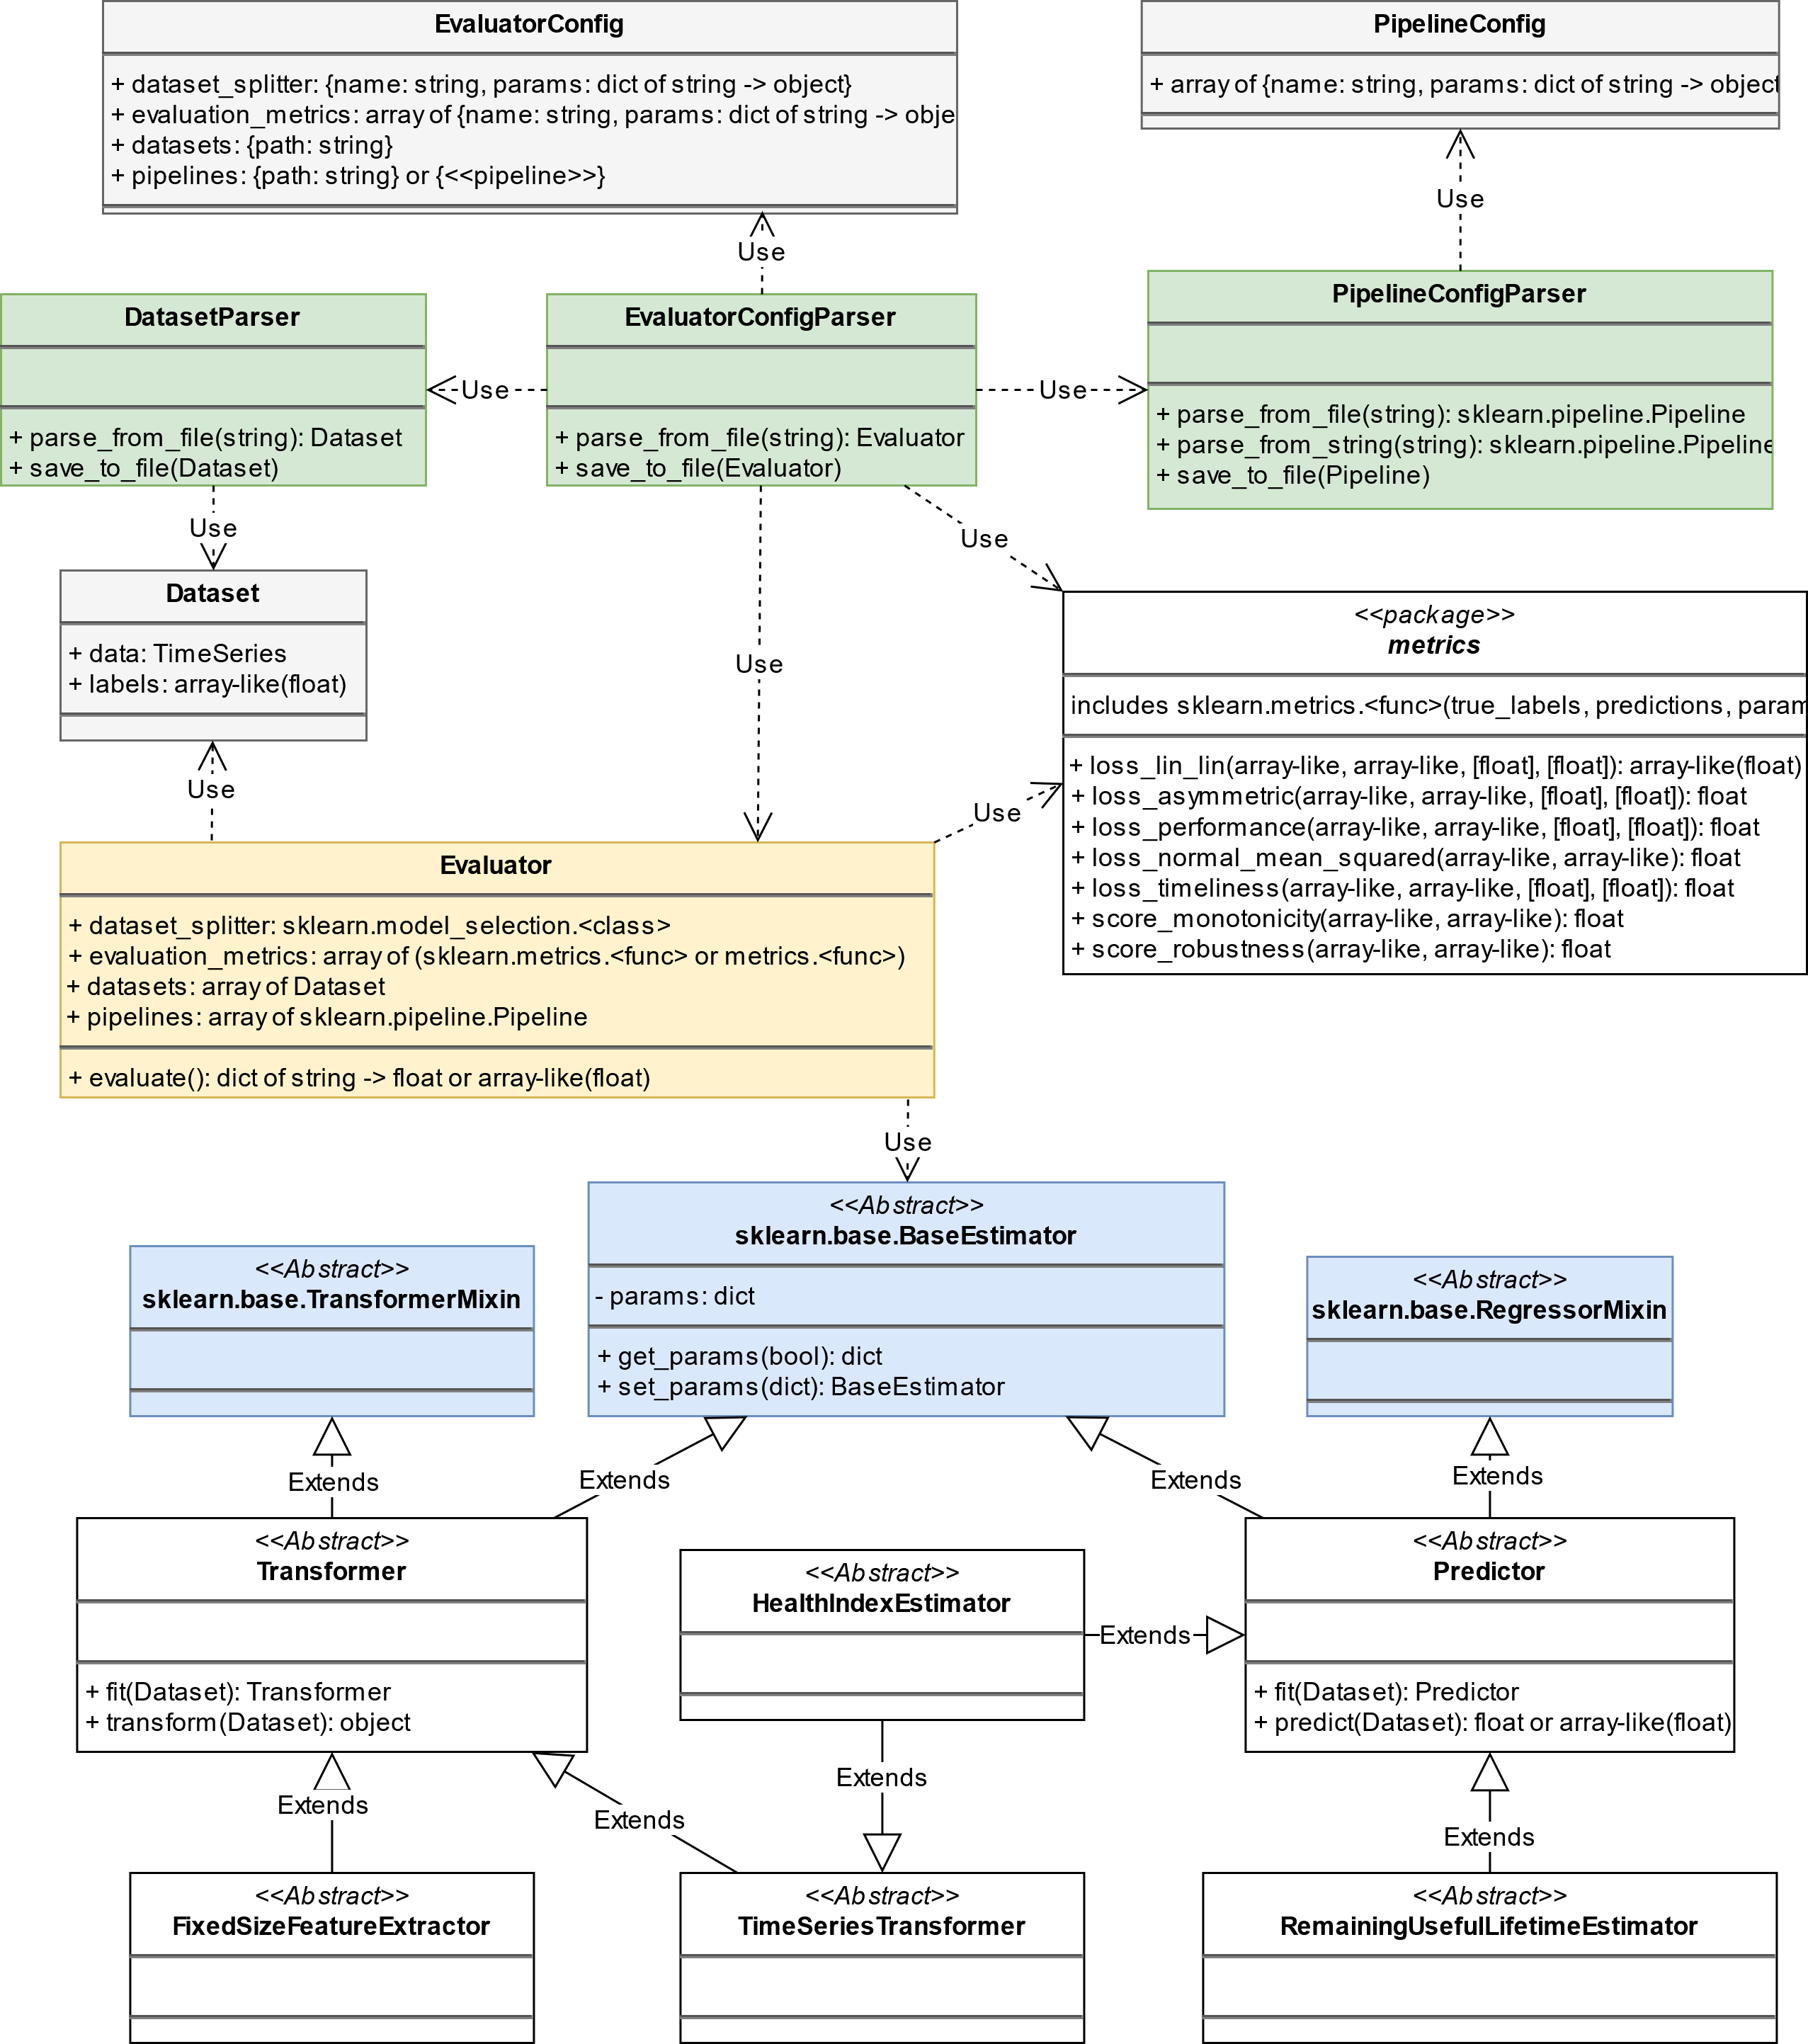
\includegraphics[width=\textwidth]{gfx/general_class_diagram}
    \caption{Class diagram showing general classes and interrelations}
    \label{fig:interfaces-general_class_diagram}
\end{figure}

\subsection*{Sequence diagram}
\vspace*{-10mm}\hfill{\fontfamily{phv}\normalsize\emph{Paul Fährmann}}
\\
The first general sequence diagram shown in Figure~\ref{fig:interfaces-general_sequence_diagram} describes the use case for loading evaluating one pipeline on one data set using the \textit{Evaluator} class. We first load the dataset via the \textit{DatasetParser}, then create a Pipeline with the \textit{make\_pipeline} call. We also create a \textit{splitter} object which is used to split the data into training and test subsets. When creating the \textit{Evaluator}, we give the dataset, the pipeline, the splitter and the metric-functions to the constructor. In the \textit{evaluate} function call of the \textit{Evaluator} object we have four nested loops.
\begin{enumerate}
    \item The first one loops over the data sets and splits them into a \textit{train\_dataset} and a \textit{test\_dataset}.
    \item In the second one we loop over the pipelines, which includes fitting the pipeline on the training set and predicting via the testing set.
    \item The third loop goes over the created splits of the data set in which the fit and the transform functions of the pipeline are called.
    \item The fourth one loops over the metrics as we now evaluate the loss or the score of the prediction for that pipeline. Here we get the \textit{evaluation\_result} back which is then concatenated or combined into the end result.
\end{enumerate}

\begin{figure}[ht]
    \centering
    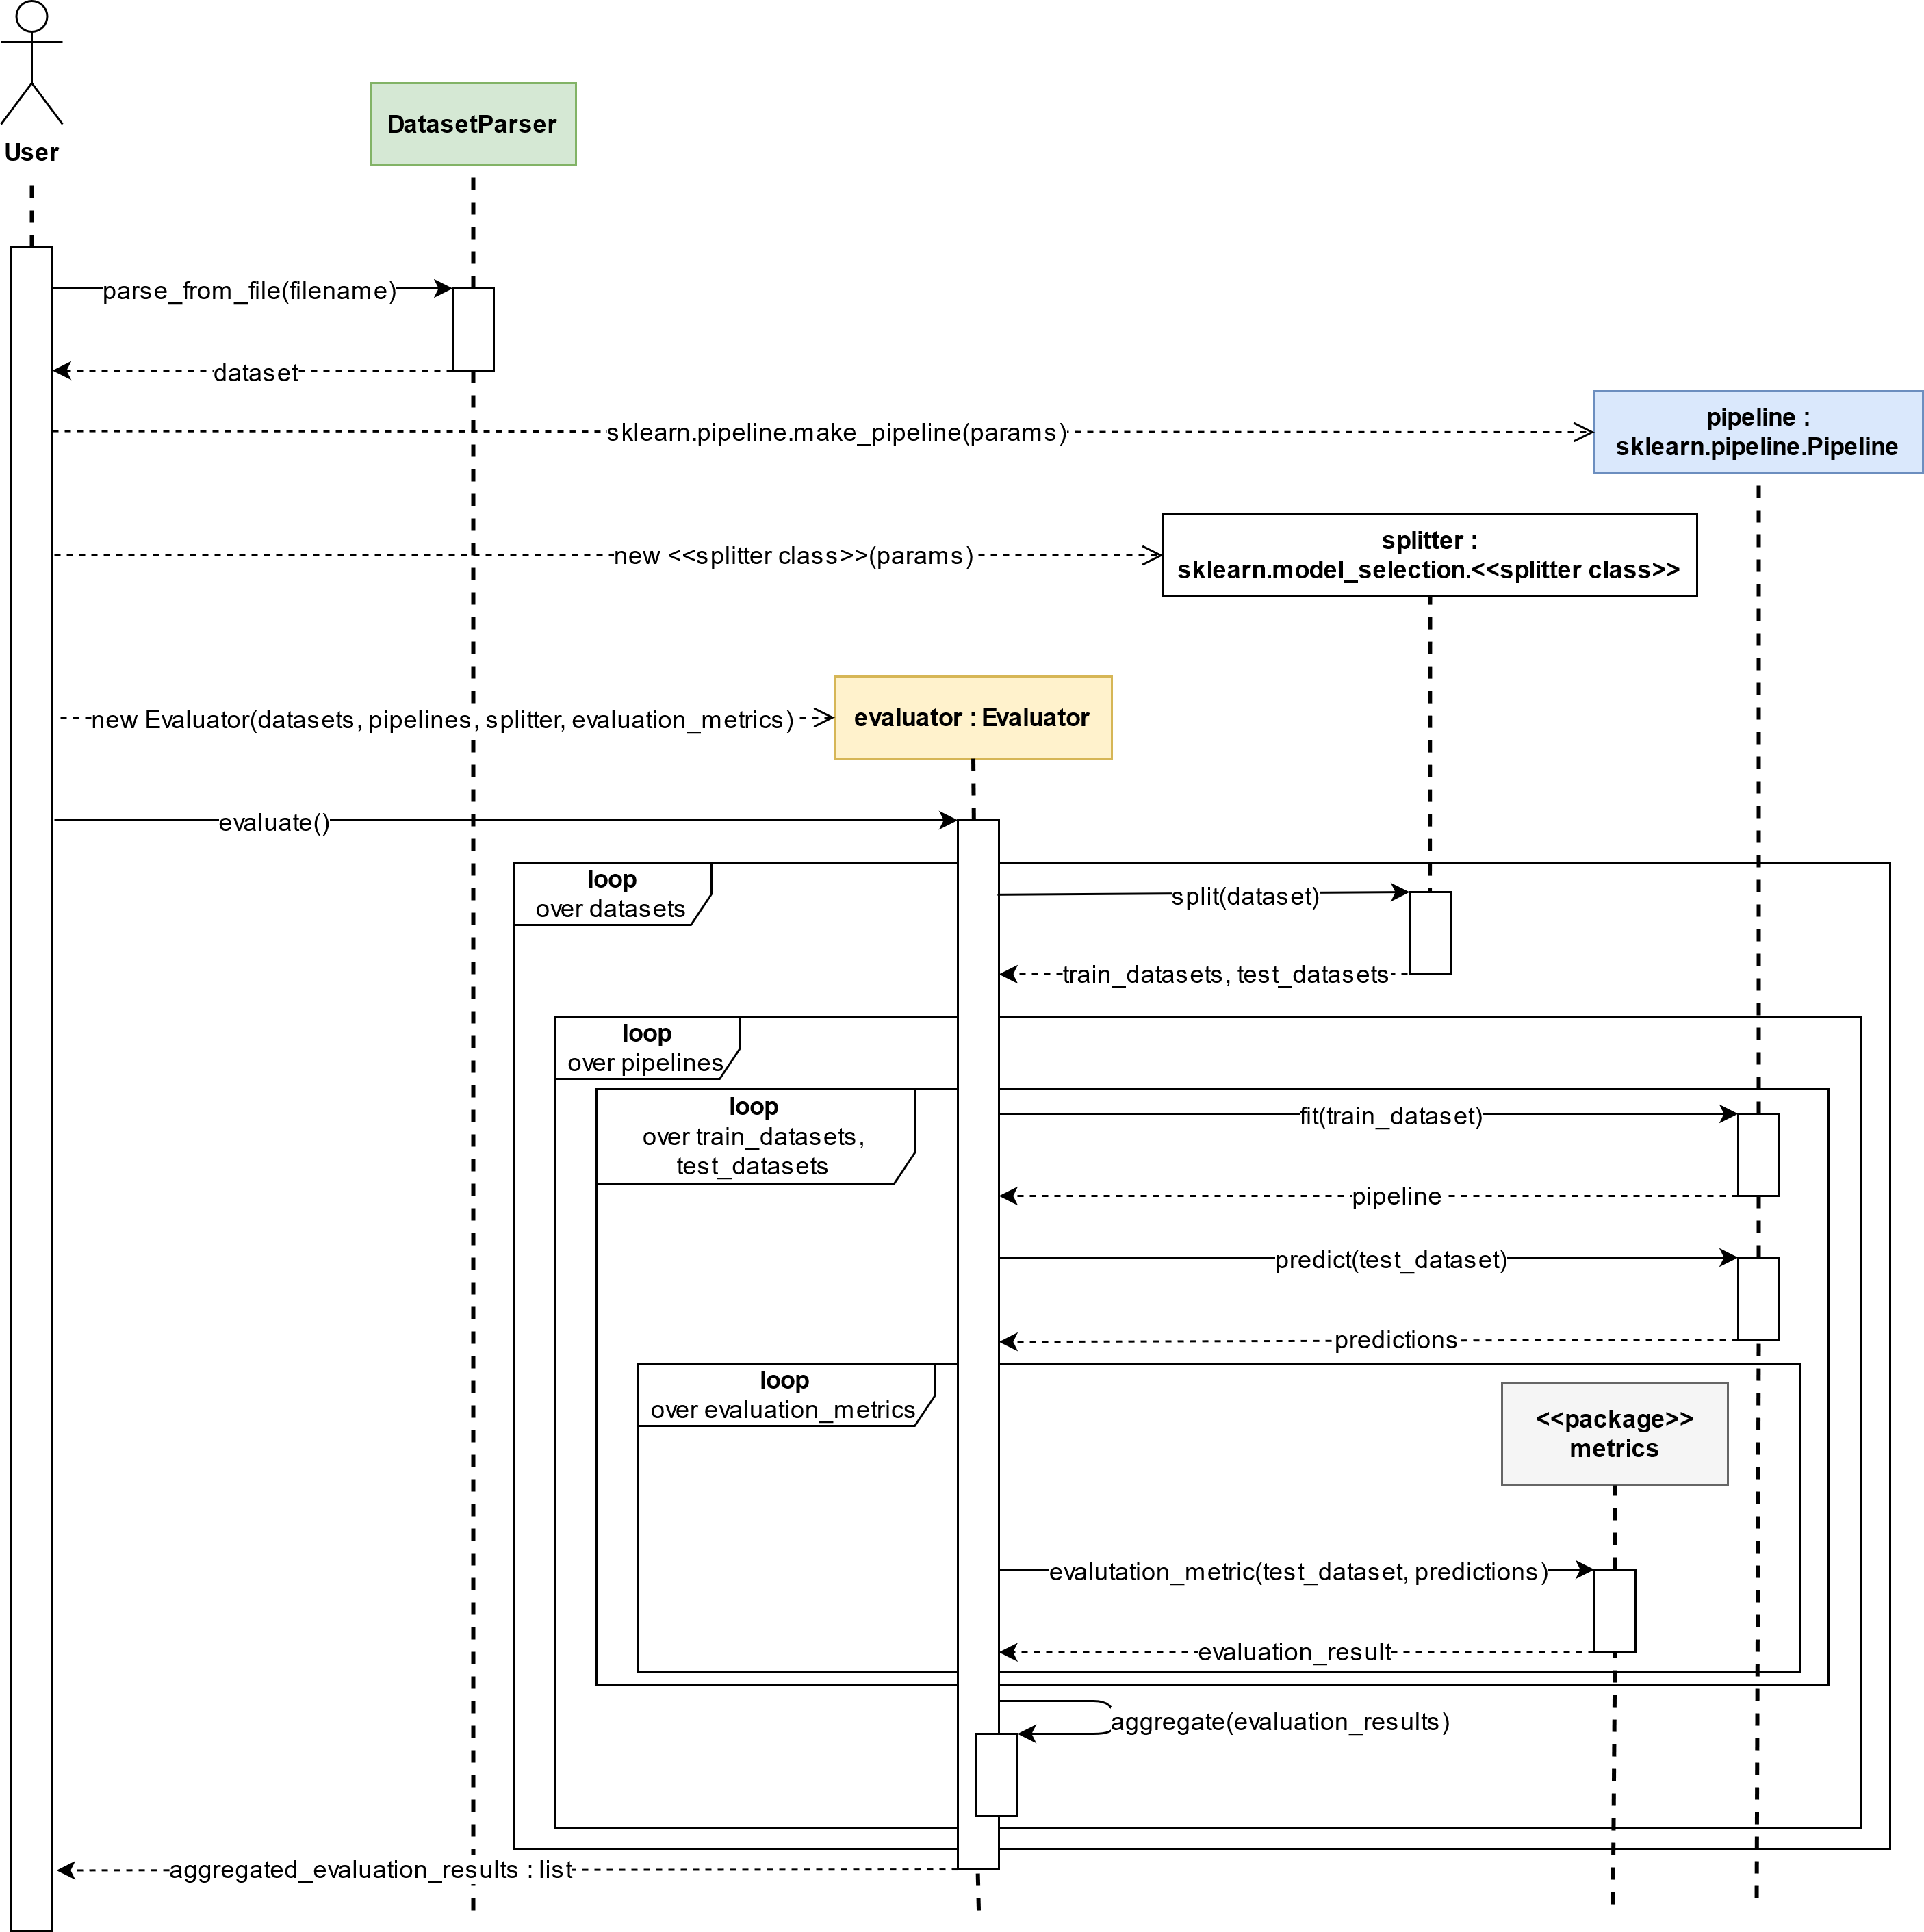
\includegraphics[width=\textwidth]{gfx/general_sequence_diagram}
    \caption{Sequence diagram showing the general flow of actions when starting from scratch.}
    \label{fig:interfaces-general_sequence_diagram}
\end{figure}

The second general sequence diagrams shown in Figure~\ref{fig:interfaces-general_sequence_diagram_with_config} describes the use case of loading an \textit{Evaluator} from a configuration file via the \textit{EvaluatorConfigParser}.
In the parsing of the configuration file the \textit{EvaluatorConfigParser} has three loops, which are however not nested.
\begin{itemize}
    \item The first loop goes over the \textit{dataset\_paths} which uses the \textit{DatasetParser} to load the datasets.
    \item The second loop goes over the \textit{pipeline\_paths} which uses the \textit{PipelineConfigParser} to load the pipeline configuration and then uses its internal pipeline parser function \textit{parse\_from\_string} to create the pipelines.
    \item The third loop goes over the pipeline configuration strings that are put into the evaluator configuration directly. These are parsed to create the pipelines.
\end{itemize}
After these loops the \textit{splitter} is created and the \textit{Evaluator} object is constructed with the now loaded datasets, pipelines, splitter and metrics, which are loaded directly.
\begin{figure}[ht]
    \centering
    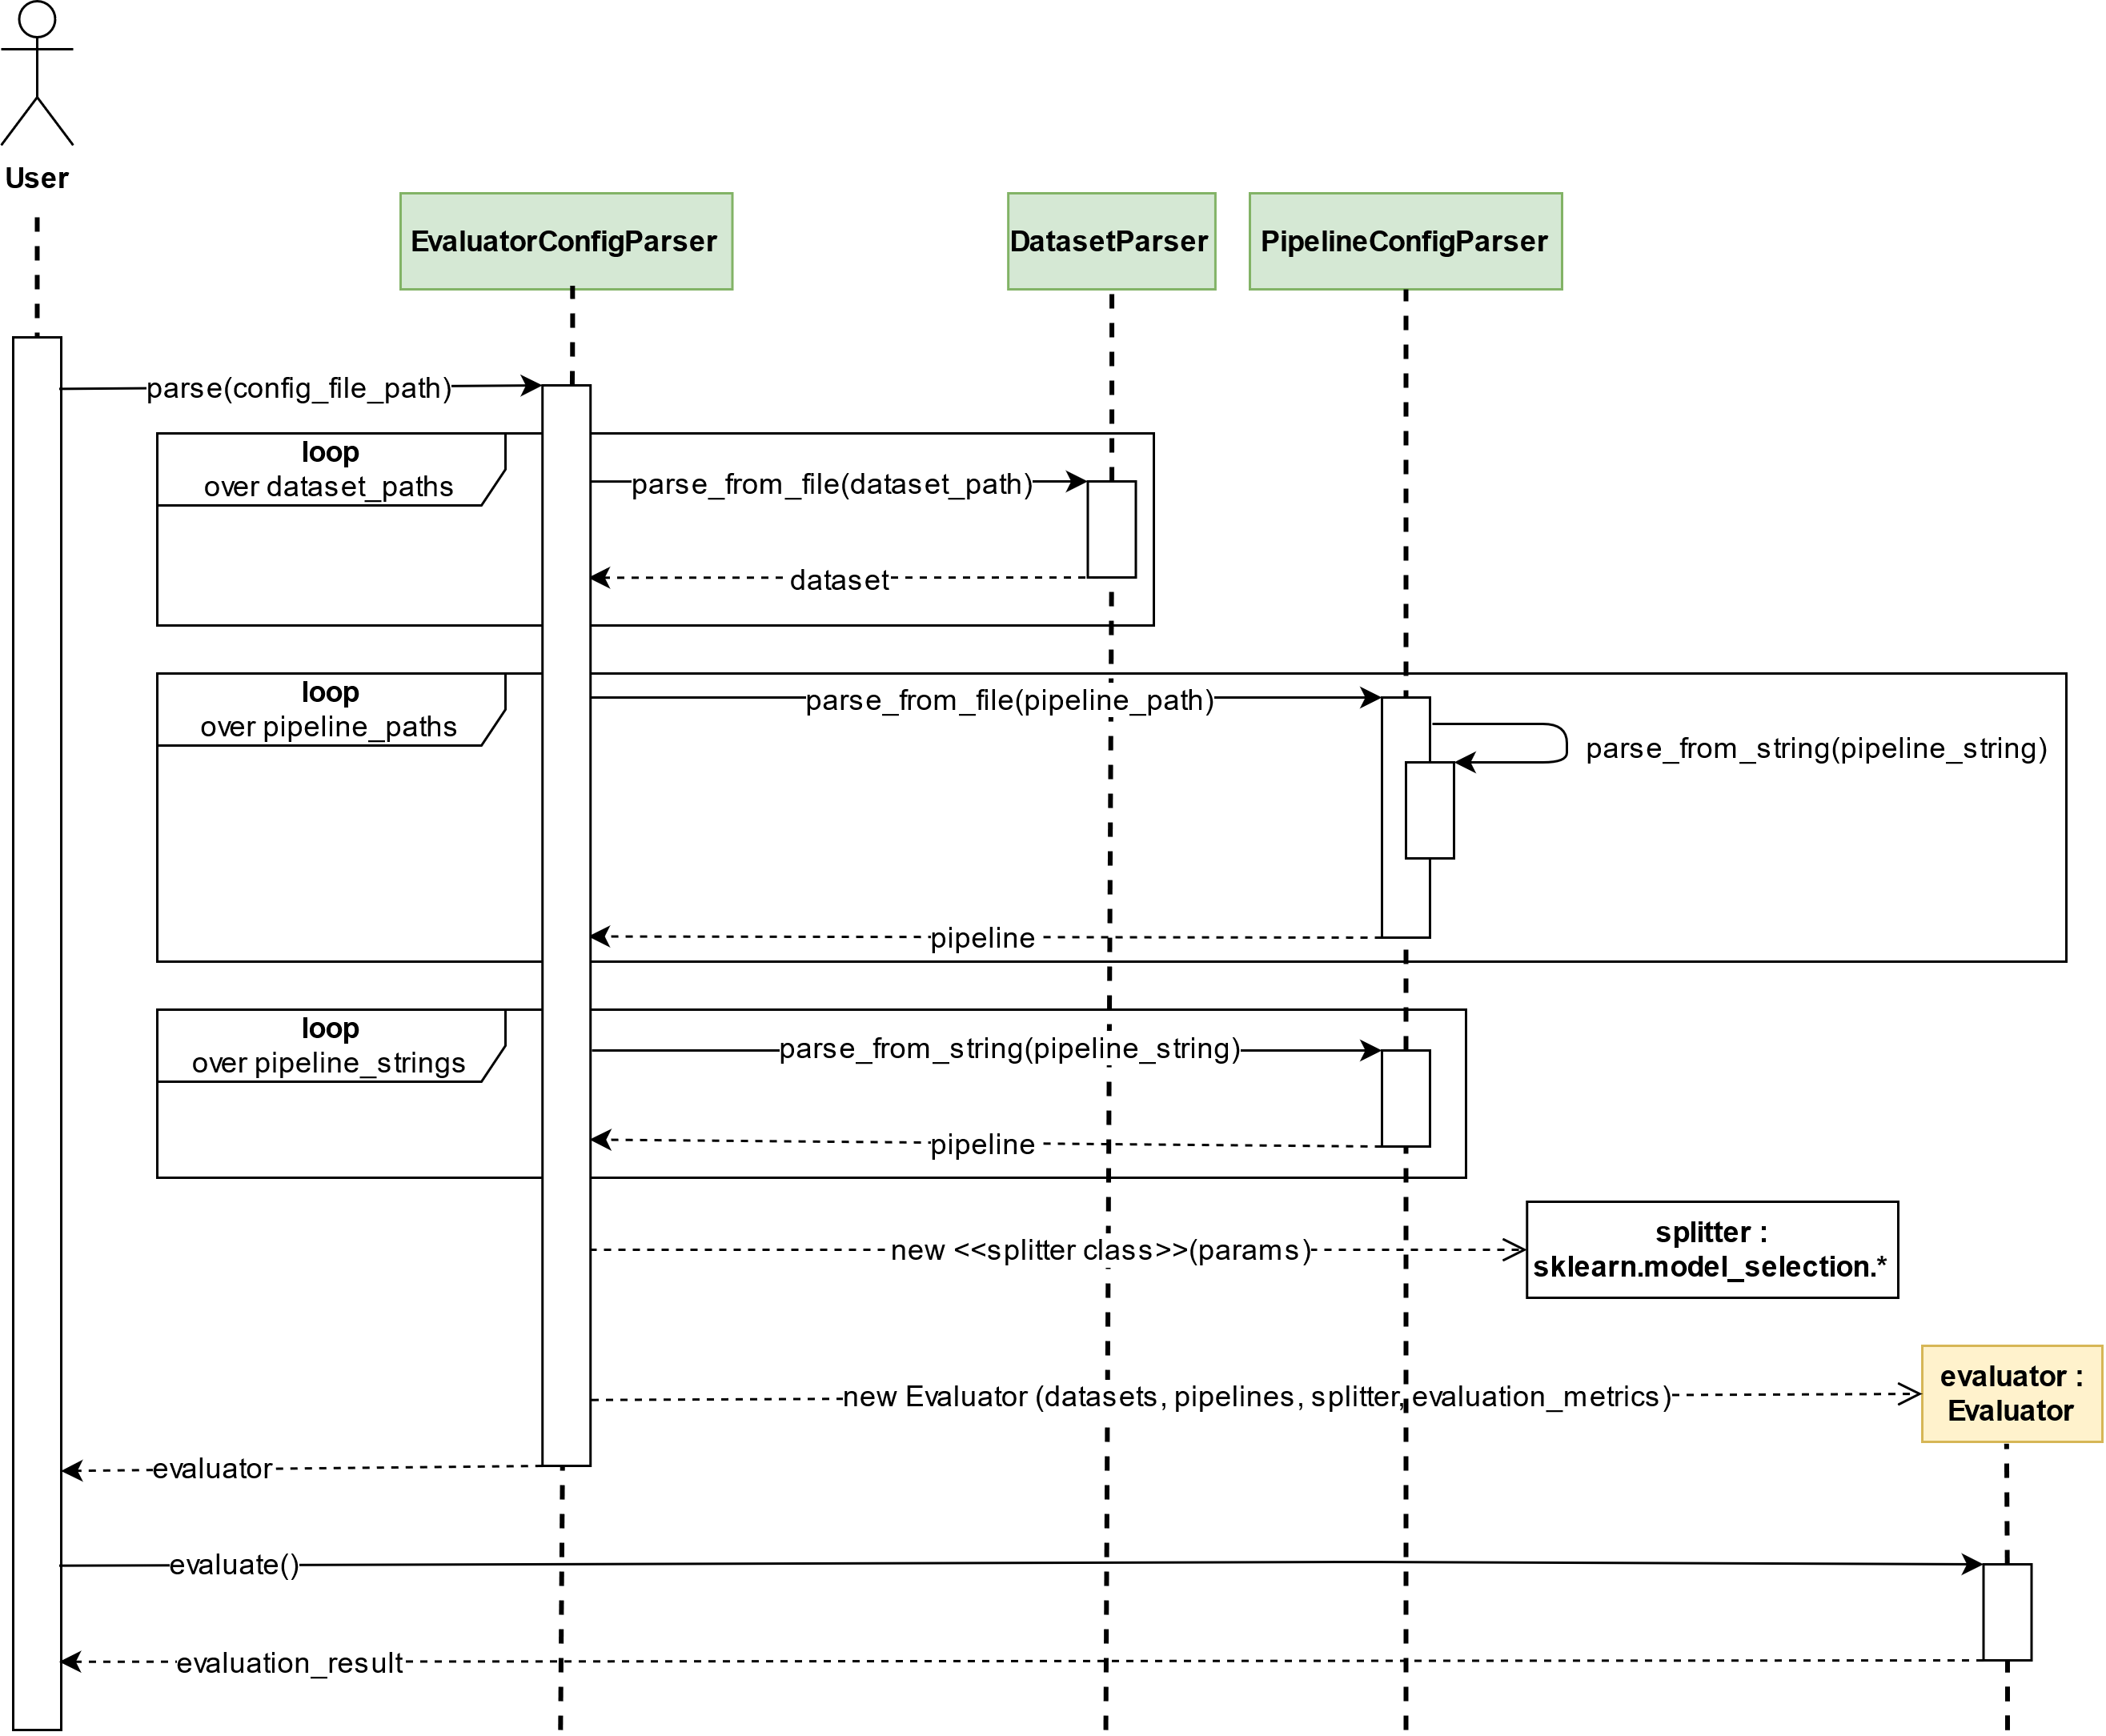
\includegraphics[width=\textwidth]{gfx/general_sequence _diagram_config}
    \caption{Sequence diagram showing the general flow of actions when starting with some predefined approach and evaluation.}
    \label{fig:interfaces-general_sequence_diagram_with_config}
\end{figure}

\section{Time Series Feature Extraction}
\vspace*{-5mm}\hfill{\fontfamily{phv}\normalsize\emph{Paul Fährmann, Sanjay Gupta}}
\\
In this chapter we show the class and sequence diagrams regarding to the classes in the feature extraction and preprocessing steps of our library.
\subsection*{Class diagram}
\vspace*{-5mm}\hfill{\fontfamily{phv}\normalsize\emph{Paul Fährmann, Sanjay Gupta}}
\\
The Figures \ref{fig:interfaces-tfe-fixedsize} and \ref{fig:interfaces-tfe-transformer} demonstrate the class diagram of time series feature extraction. Every class that inherits from the \textit{FixedSizeFeatureExtractor} abstract class transforms a time series into a fixed length vector of real valued features. These are \textit{RNNAutoencoder} which represents a time series into a fixed dimension using neuronal networks, \textit{TSFreshWrapper} which extracts basic statistical features, \textit{PytsTransformWrapper} which includes several methods of extracting feature vectors and \textit{MovingWeightedAverage} which calculates one moving weighted value of a time series.

\begin{figure}[ht]
    \centering
    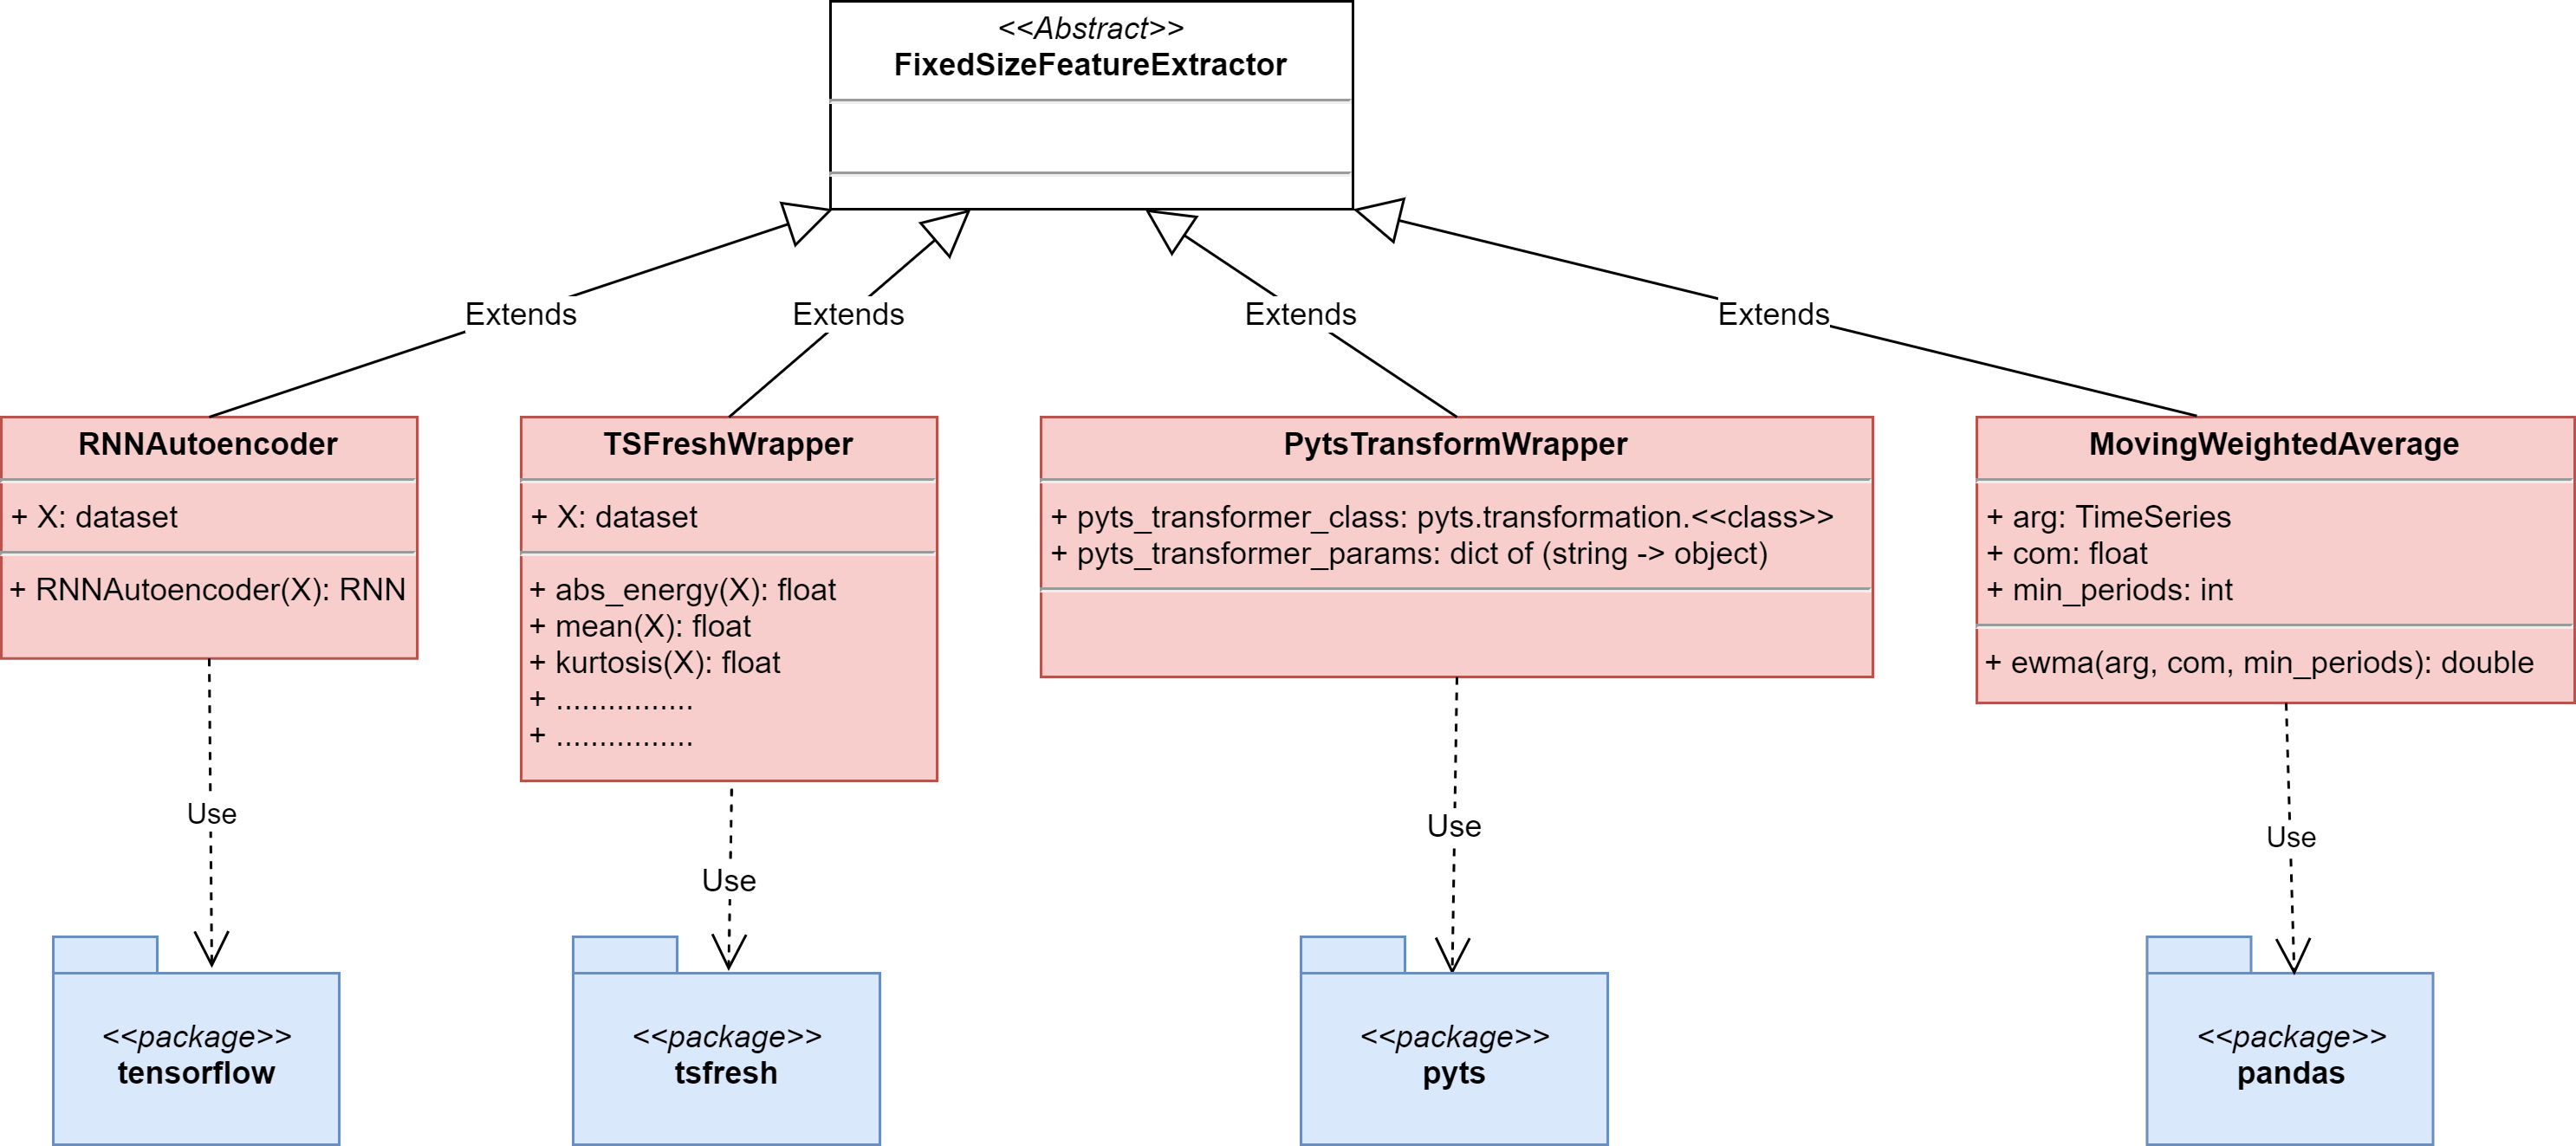
\includegraphics[width=\textwidth]{gfx/Interfaces-TFE-FixedSize.png}
    \caption{Class diagram of Fixed size feature extractor.}
    \label{fig:interfaces-tfe-fixedsize}
\end{figure}
Every class that inherits from the \textit{TimeSeriesTransformer} abstract class transforms a time series into another time series. These are the \textit{TimeSeriesImputer} which imputes timestamp-value pairs, \textit{EMDSignalWrapper} and \textit{PywtWrapper} which extract and filter the time series and the \textit{WindowingApproach} which cuts the time series into same size chunks.
\begin{figure}[ht]
    \centering
    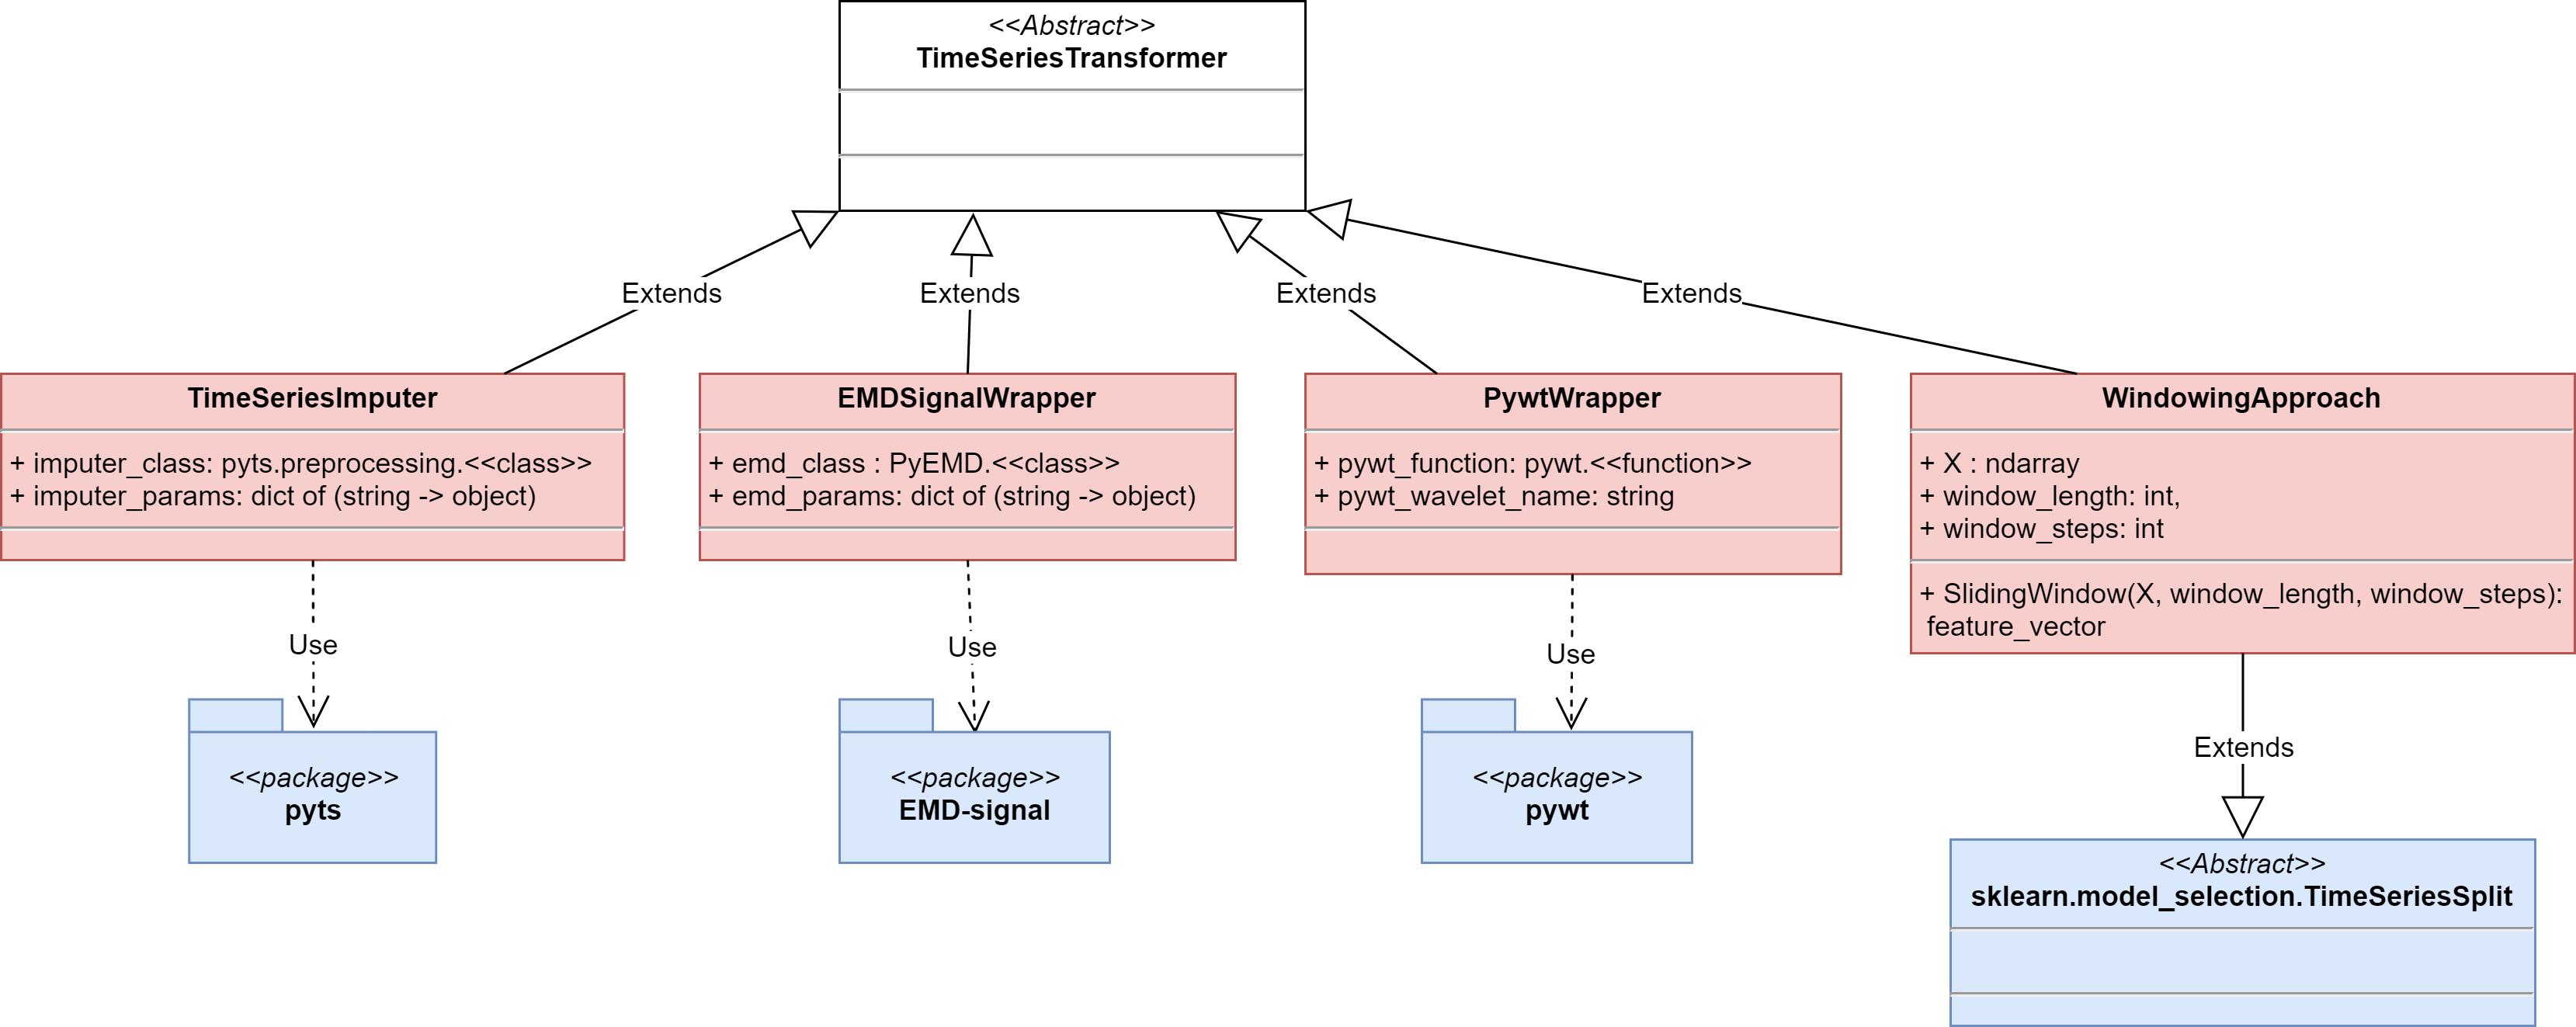
\includegraphics[width=\textwidth]{gfx/Interfaces-TFE-Transformer.png}
    \caption{Class diagram of Time Series Transformer.}
    \label{fig:interfaces-tfe-transformer}
\end{figure}
The \textit{UniToMultivariateWrapper} class applies the specified transformer on all time series. The transformers class can either be a \textit{TimeSeriesTransformer} or a \textit{FixedSizeFeatureExtractor}.
\begin{figure}[ht]
    \centering
    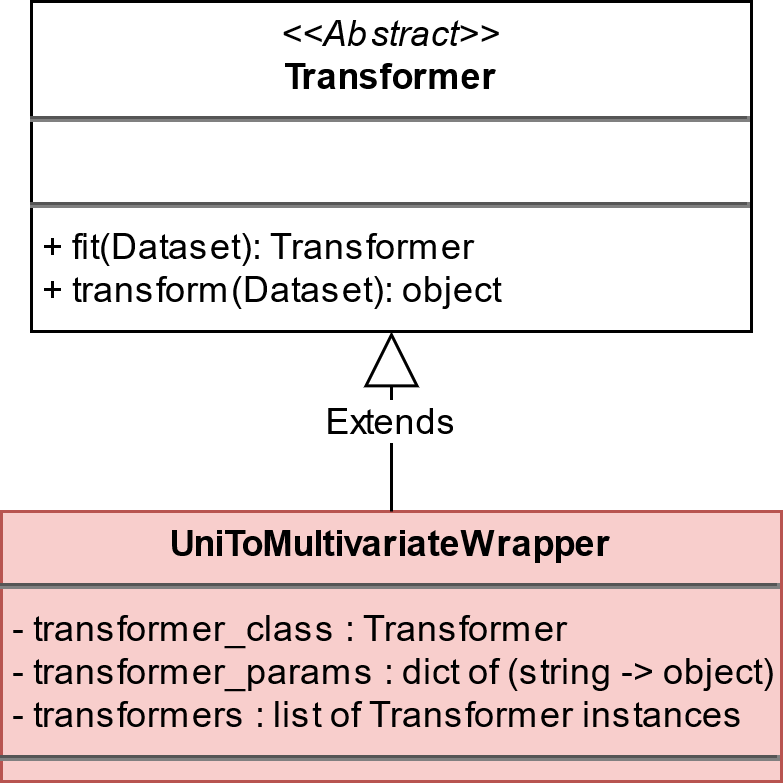
\includegraphics[width=.4\textwidth]{gfx/uni_to_multivariate_wrapper_class}
    \caption{Class diagram showing general classes and interrelations}
    \label{fig:interfaces-tfe-unitomulti}
\end{figure}
\newpage
\subsection*{Sequence diagram}
We are explaining the fit and transform use cases for the different time series feature extraction and preprocessing classes.
\subsubsection*{UniToMultivariateWrapper}
\vspace*{-10mm}\hfill{\fontfamily{phv}\normalsize\emph{Paul Fährmann}}
\\
The \textit{UniToMultivariateWrapper} applies a transformation to each sensor data (univariate time series) of the dataset and aggregates the transformed data at the end. We specify the used \textit{transformer\_class} with the \textit{transformer\_params} in the constructor.
\begin{figure}[ht]
    \centering
    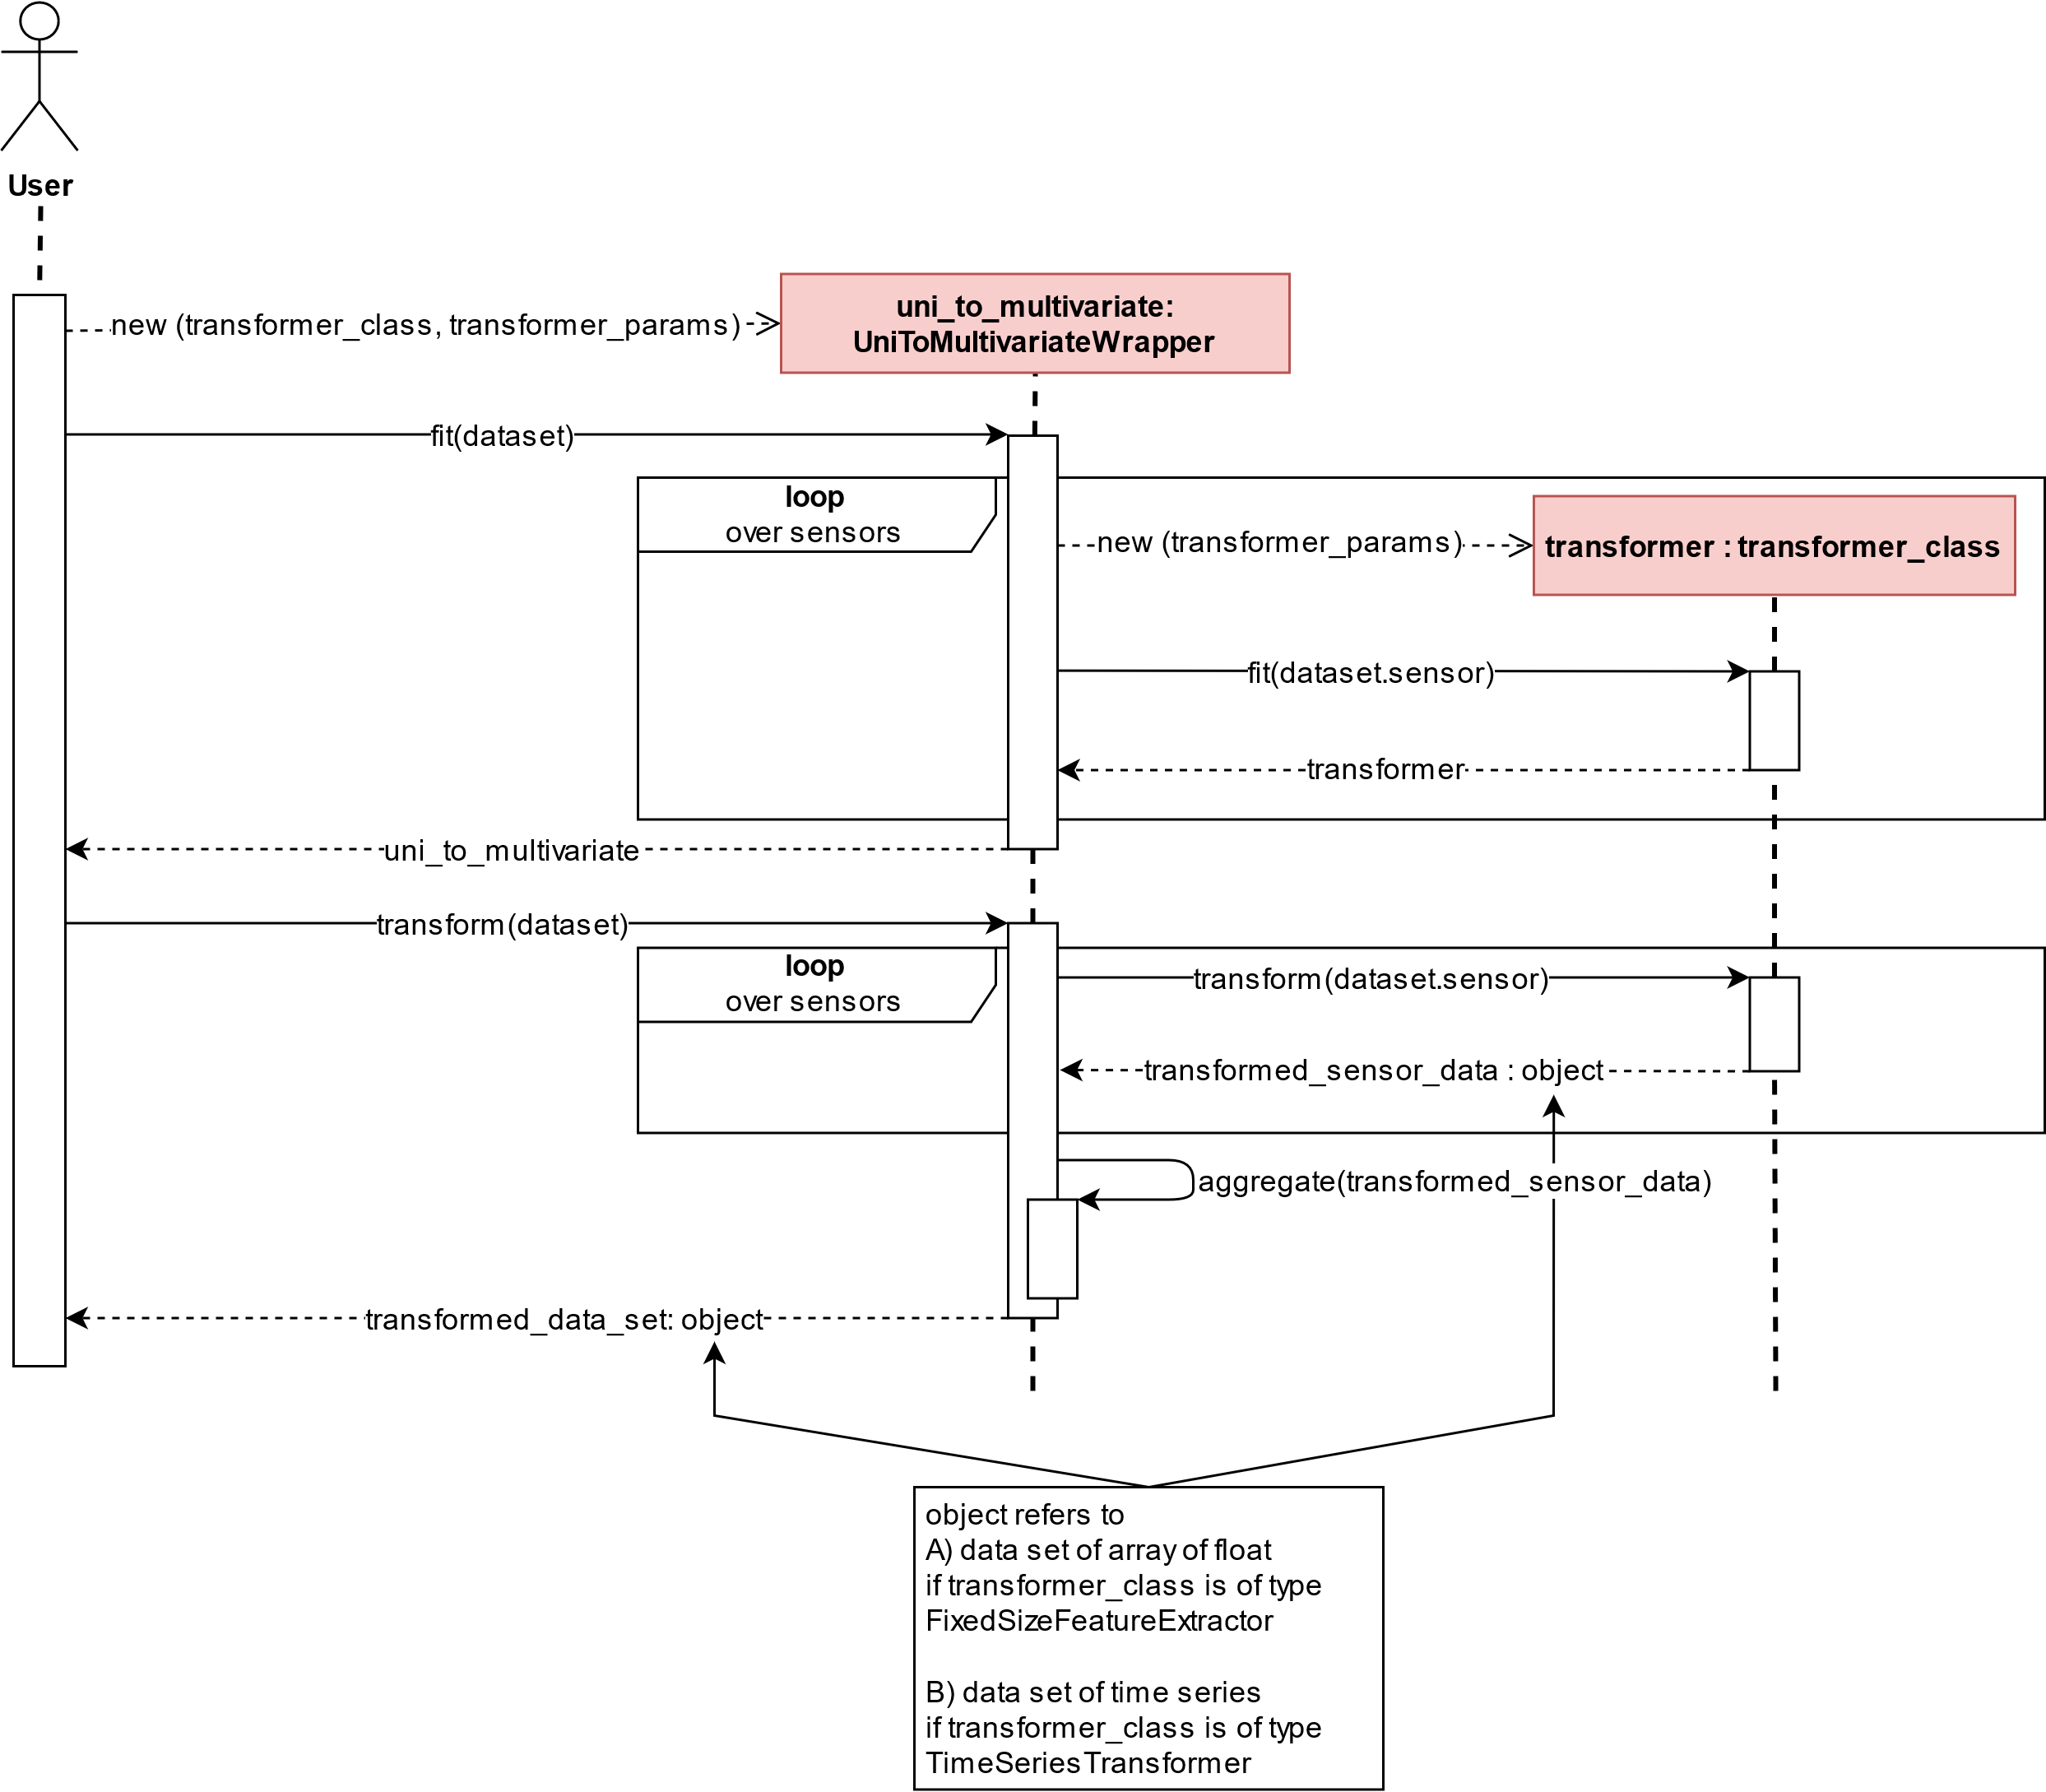
\includegraphics[width=\textwidth]{gfx/uni_to_multi_sequence}
    \caption{Sequence Diagram of the UniToMultivariateWrapper class for fit and transform use-case.}
    \label{fig:uni-to-multi-seq}
\end{figure}
In Figure~\ref{fig:uni-to-multi-seq}, we show the use case for the fit and the transform function call. In the fit call we loop over the sensors and create a transformer object for each sensor respectively and also call the fit function on that transformer. These transformers are saved in a list \textit{transformers} as member parameters. In the \textit{transform} function call we again loop over the sensors and call the transform on the fitted transformer for that sensor from our list of transformers. After transforming these sensors we aggregate the result. If our specified transformer class is of type \textit{TimeSeriesTransformer} we transform each individual sensor time series into the new form for an instance of the dataset. If our specified transformer class is of type \textit{FixedSizeFeatureExtractor} we concatenate the resulting fixed size vectors of the sensors to one vector for an instance of the dataset.
\subsubsection*{PywtWrapper}
\vspace*{-10mm}\hfill{\fontfamily{phv}\normalsize\emph{Paul Fährmann}}
\\
The \textit{PywtWrapper} is a wrapper for the PyWavelet library \textit{pywt}\footnote{\href{https://pywavelets.readthedocs.io/en/latest/}{https://pywavelets.readthedocs.io/en/latest/}}. The \textit{pywt} package contains several wavelet transformation functions that scan over the time and frequency domain of the data. We specify the used transformation function \textit{pywt\_function} and the wavelet function name \textit{pywt\_wavelet\_name} in the constructor of the \textit{PywtWrapper}. In Figure~\ref{fig:tfe-pywt-seq}, we show the use case for the fit and the transform function call. In the fit call nothing happens, as nothing from the dataset needs to be known before. In the transform function call, the specified wavelet transformation function is called with the dataset and the specified wavelet function. We get back the wavelet-coefficients.
\begin{figure}[ht]
    \centering
    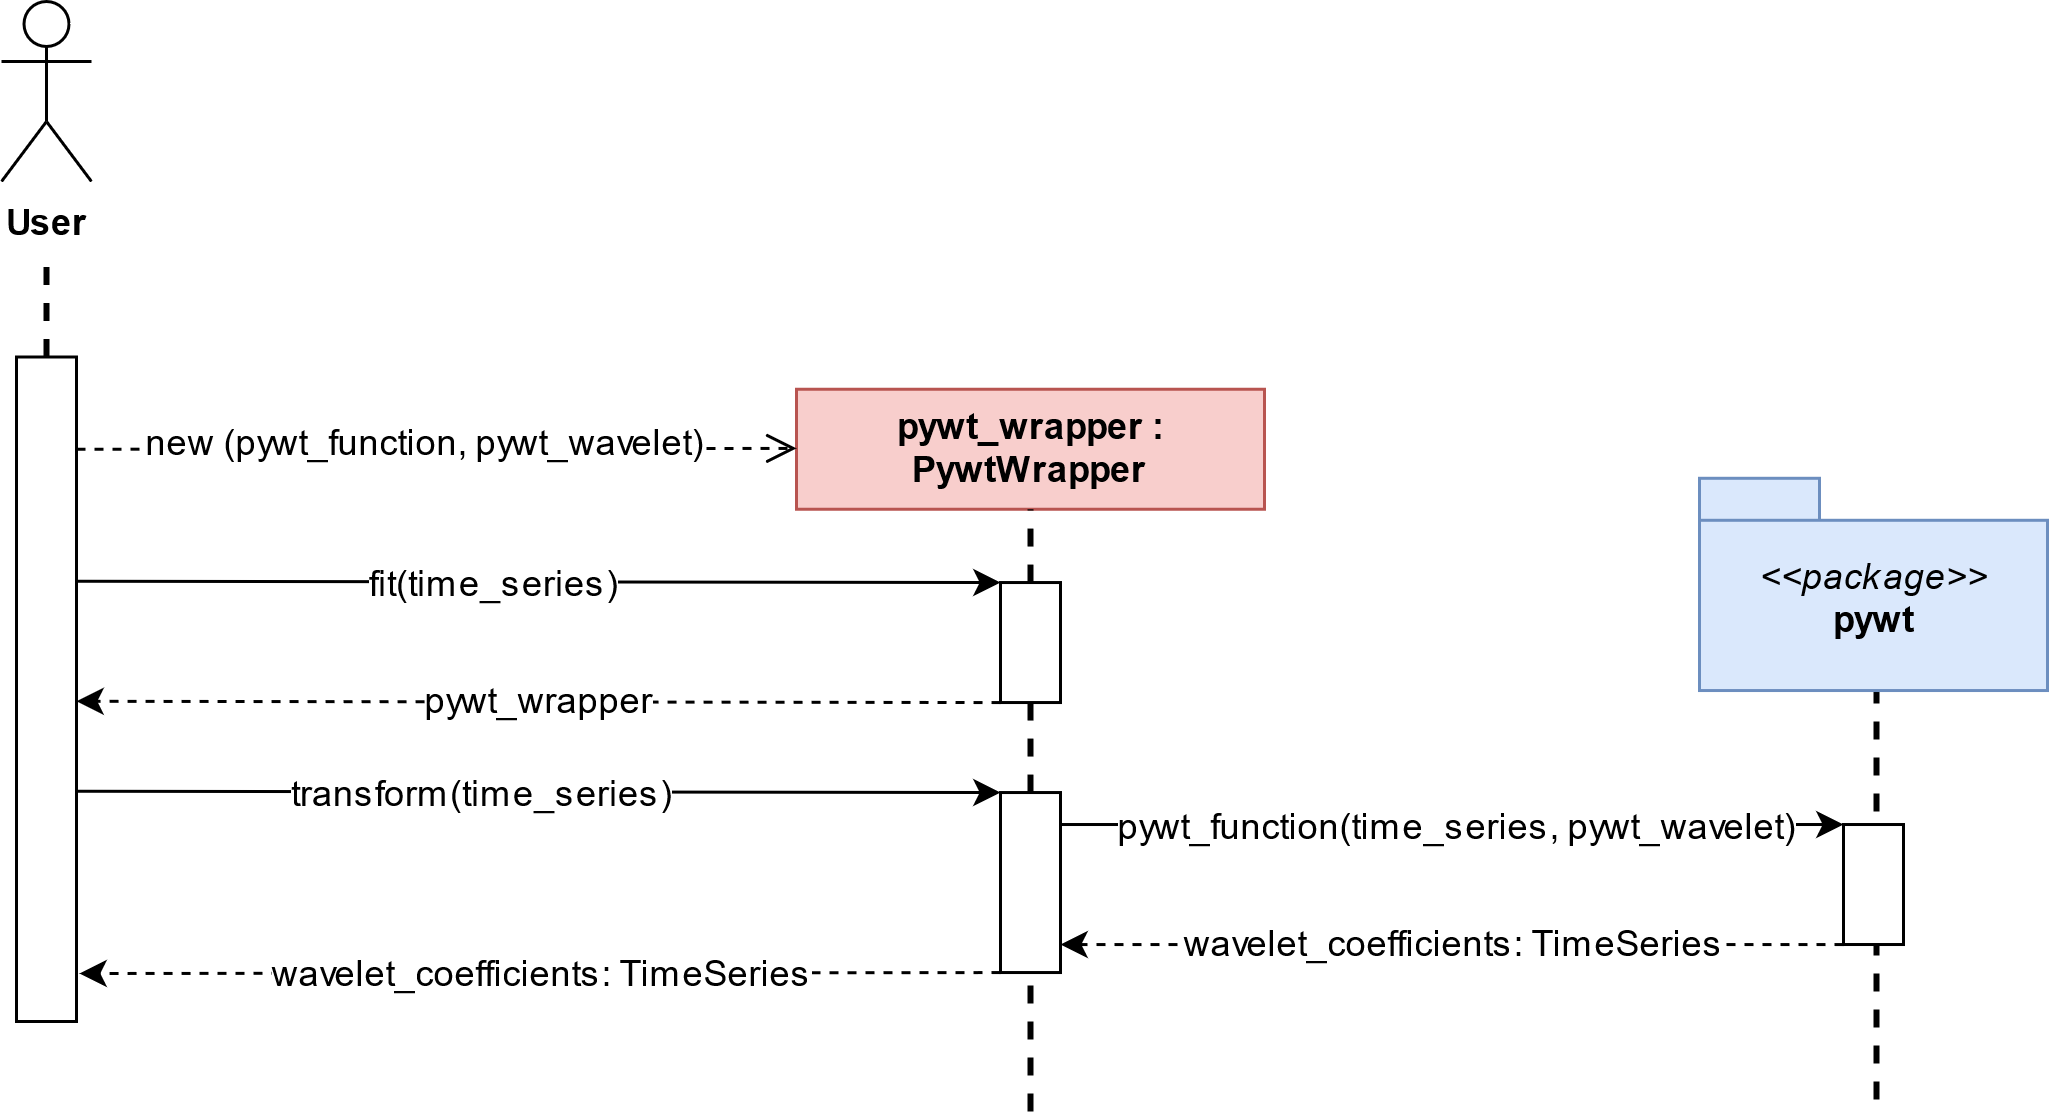
\includegraphics[width=\textwidth]{gfx/pywt_sequence}
    \caption{Sequence Diagram of the PywtWrapper class for fit and transform use-case.}
    \label{fig:tfe-pywt-seq}
\end{figure}
\newpage
\subsubsection*{EMDSignalWrapper}
\vspace*{-10mm}\hfill{\fontfamily{phv}\normalsize\emph{Paul Fährmann}}
\\
The \textit{EMDSignalWrapper} is a wrapper for the EMD-Signal library \textit{PyEMD}\footnote{\href{https://pypi.org/project/EMD-signal/}{https://pypi.org/project/EMD-signal/}}. This library contains several EMD classes. We specify the used class of that library and the constructor parameters in the \textit{EMDSignalWrapper} constructor and create the \textit{emd\_class} object with the specified params. In Figure~\ref{fig:tfe-emd-signal-seq}, we show the use case for the fit and the transform function call. The fit function call does nothing, but in the transform call, the emd object is used to calculate the imf components for the time series in given dataset.
\begin{figure}[ht]
    \centering
    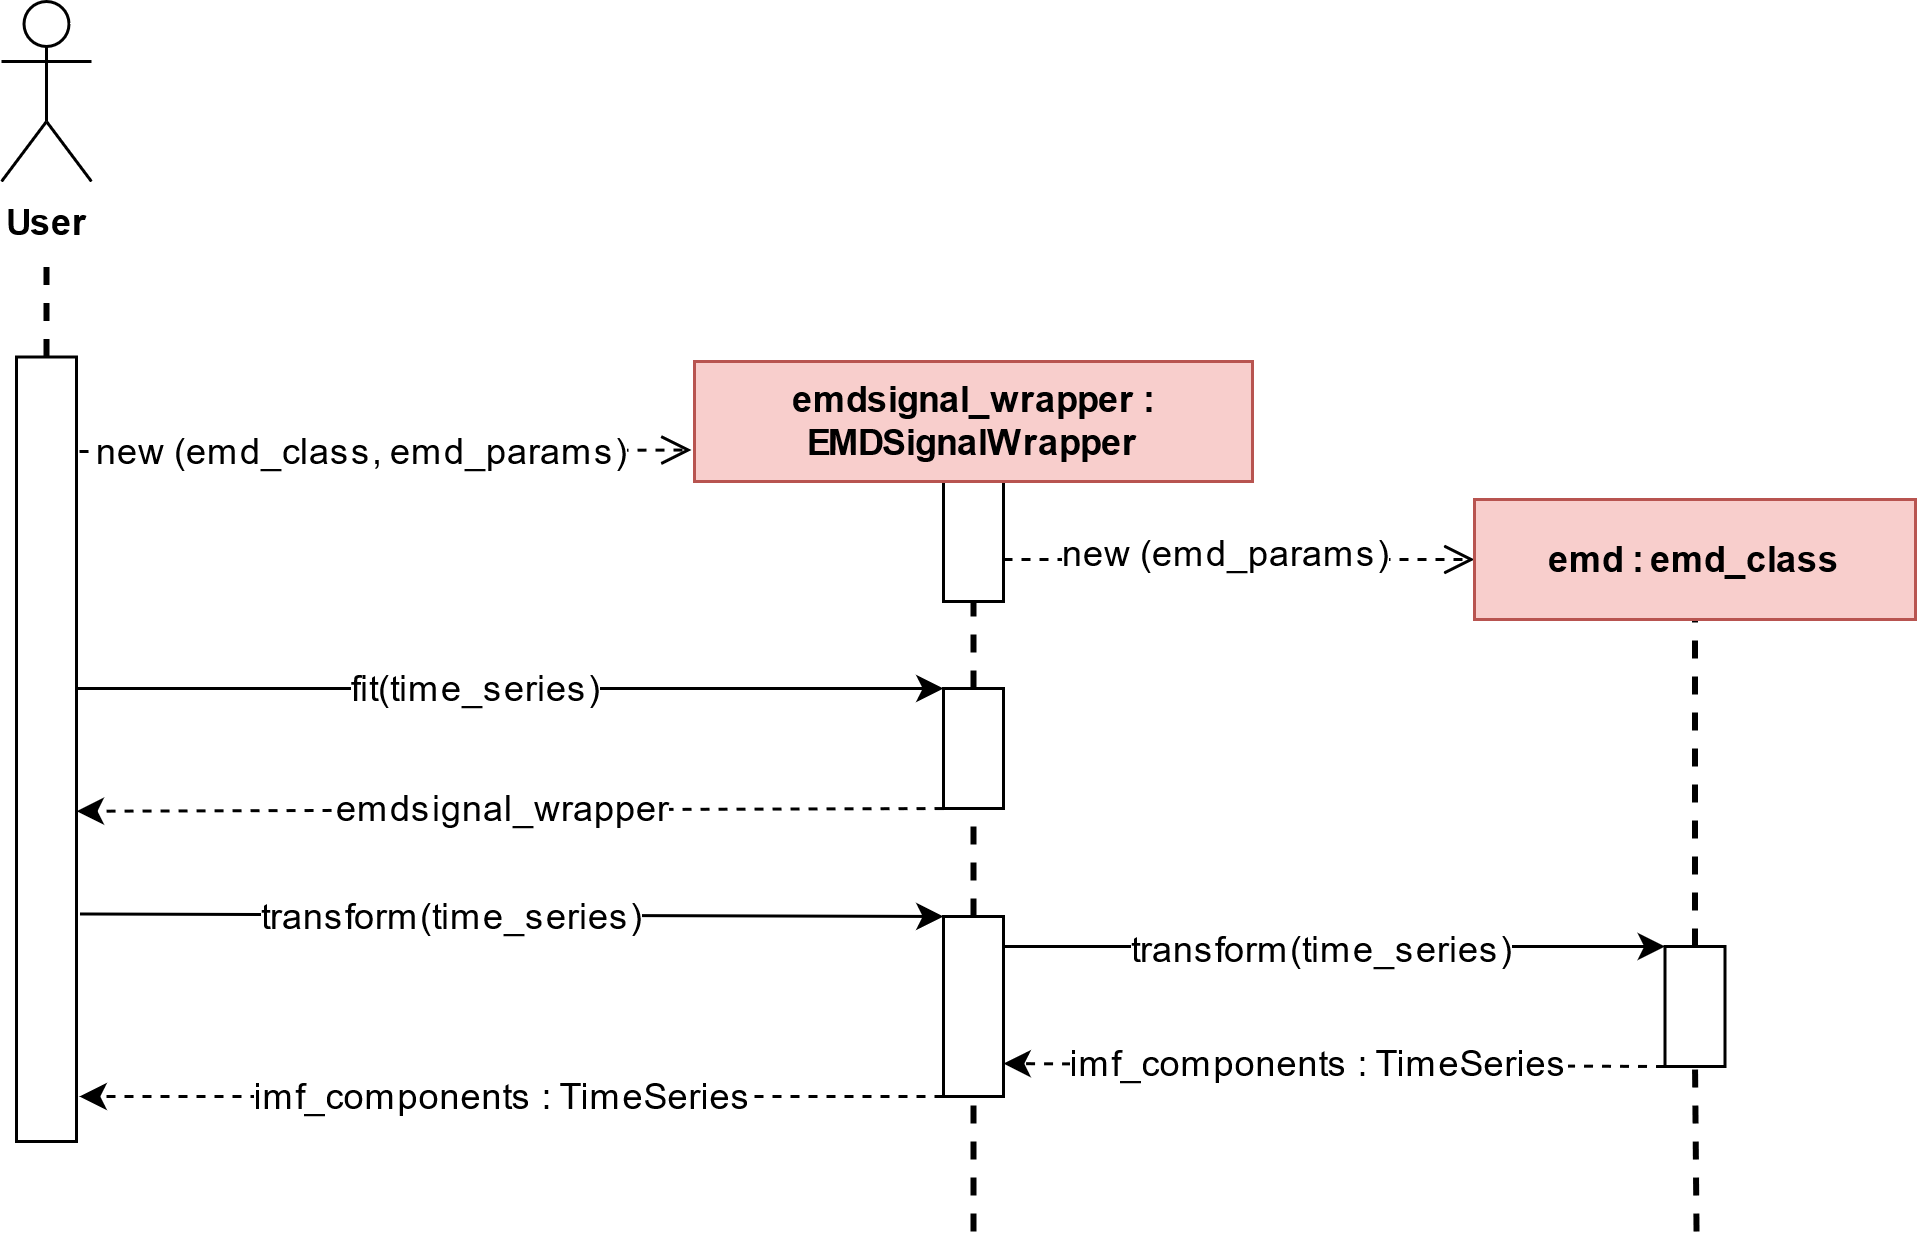
\includegraphics[width=\textwidth]{gfx/emdsignal_sequence}
    \caption{Sequence Diagram of the EMDSignalWrapper class for fit and transform use-case.}
    \label{fig:tfe-emd-signal-seq}
\end{figure}
\subsubsection*{TimeSeriesImputer}
\vspace*{-10mm}\hfill{\fontfamily{phv}\normalsize\emph{Paul Fährmann}}
\\
The \textit{TimeSeriesImputer} is a wrapper for the \textit{pyts.preprocessing}\footnote{\href{https://pypi.org/project/pyts/}{https://pypi.org/project/pyts/}} imputer classes that can be extended in the implementation phase to a more general imputer for time series, hence the name. We specify the class and the constructor params of the imputer class in the \textit{PytsImputeWrapper} constructor and create the \textit{pyts\_imputer\_class} object with the specified params. In Figure~\ref{fig:tfe-pyts-impute-seq}, we show the use case for the fit and the transform function call. In the \textit{fit} call we call the fit function of that imputer and get back the imputer. In the \textit{transform} call we just call the transform function of the imputer class object.
\begin{figure}[ht]
    \centering
    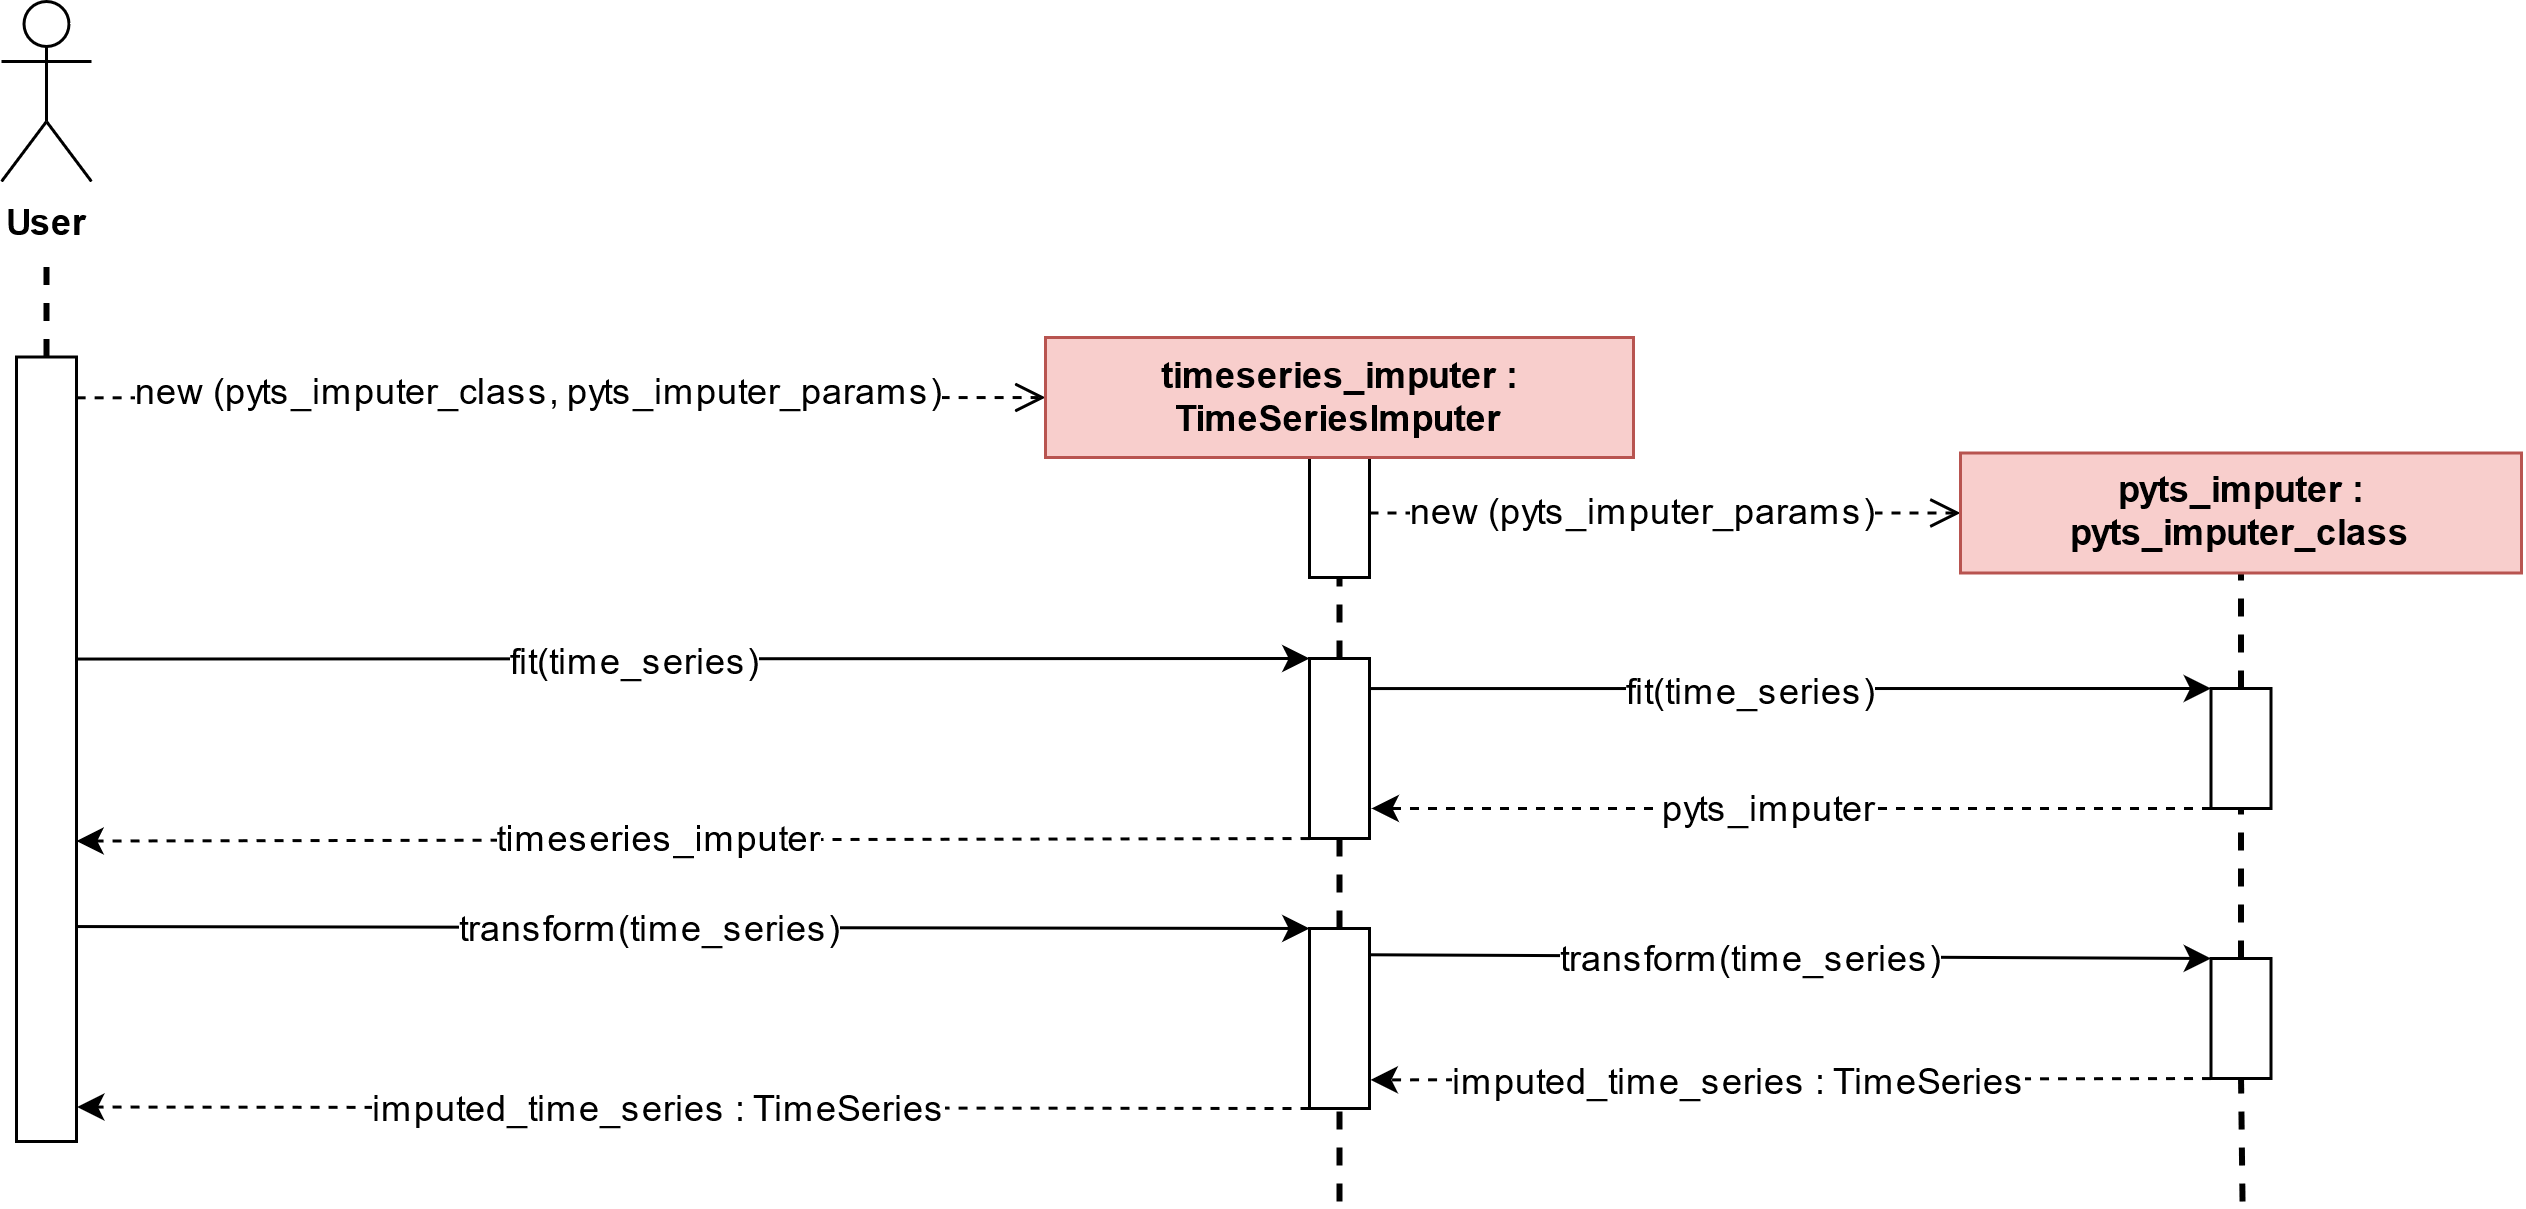
\includegraphics[width=\textwidth]{gfx/pyts_imputer_sequence}
    \caption{Sequence Diagram of the PytsImputeWrapper class for fit and transform use-case.}
    \label{fig:tfe-pyts-impute-seq}s
\end{figure}
\subsubsection*{PytsTransformWrapper}
\vspace*{-10mm}\hfill{\fontfamily{phv}\normalsize\emph{Paul Fährmann and Sanjay Gupta}}
\\
The \textit{PytsTransformWrapper} is a wrapper for the \textit{pyts.transform}\footnote{\href{https://pypi.org/project/pyts/}{https://pypi.org/project/pyts/}} classes. We specify the class and the constructor params of the transformer class in the \textit{PytsTransformWrapper} constructor and create the \textit{pyts\_transformer\_class} object with the specified params. In Figure~\ref{fig:tfe-pyts-transform-seq}, we show the use case for the fit and the transform function call. In the \textit{fit} call we call the fit function of that transformer and get back the \textit{pyts\_transformer}. In the \textit{transform} call we just call the transform function of the transformer class object.
\begin{figure}[ht]
    \centering
    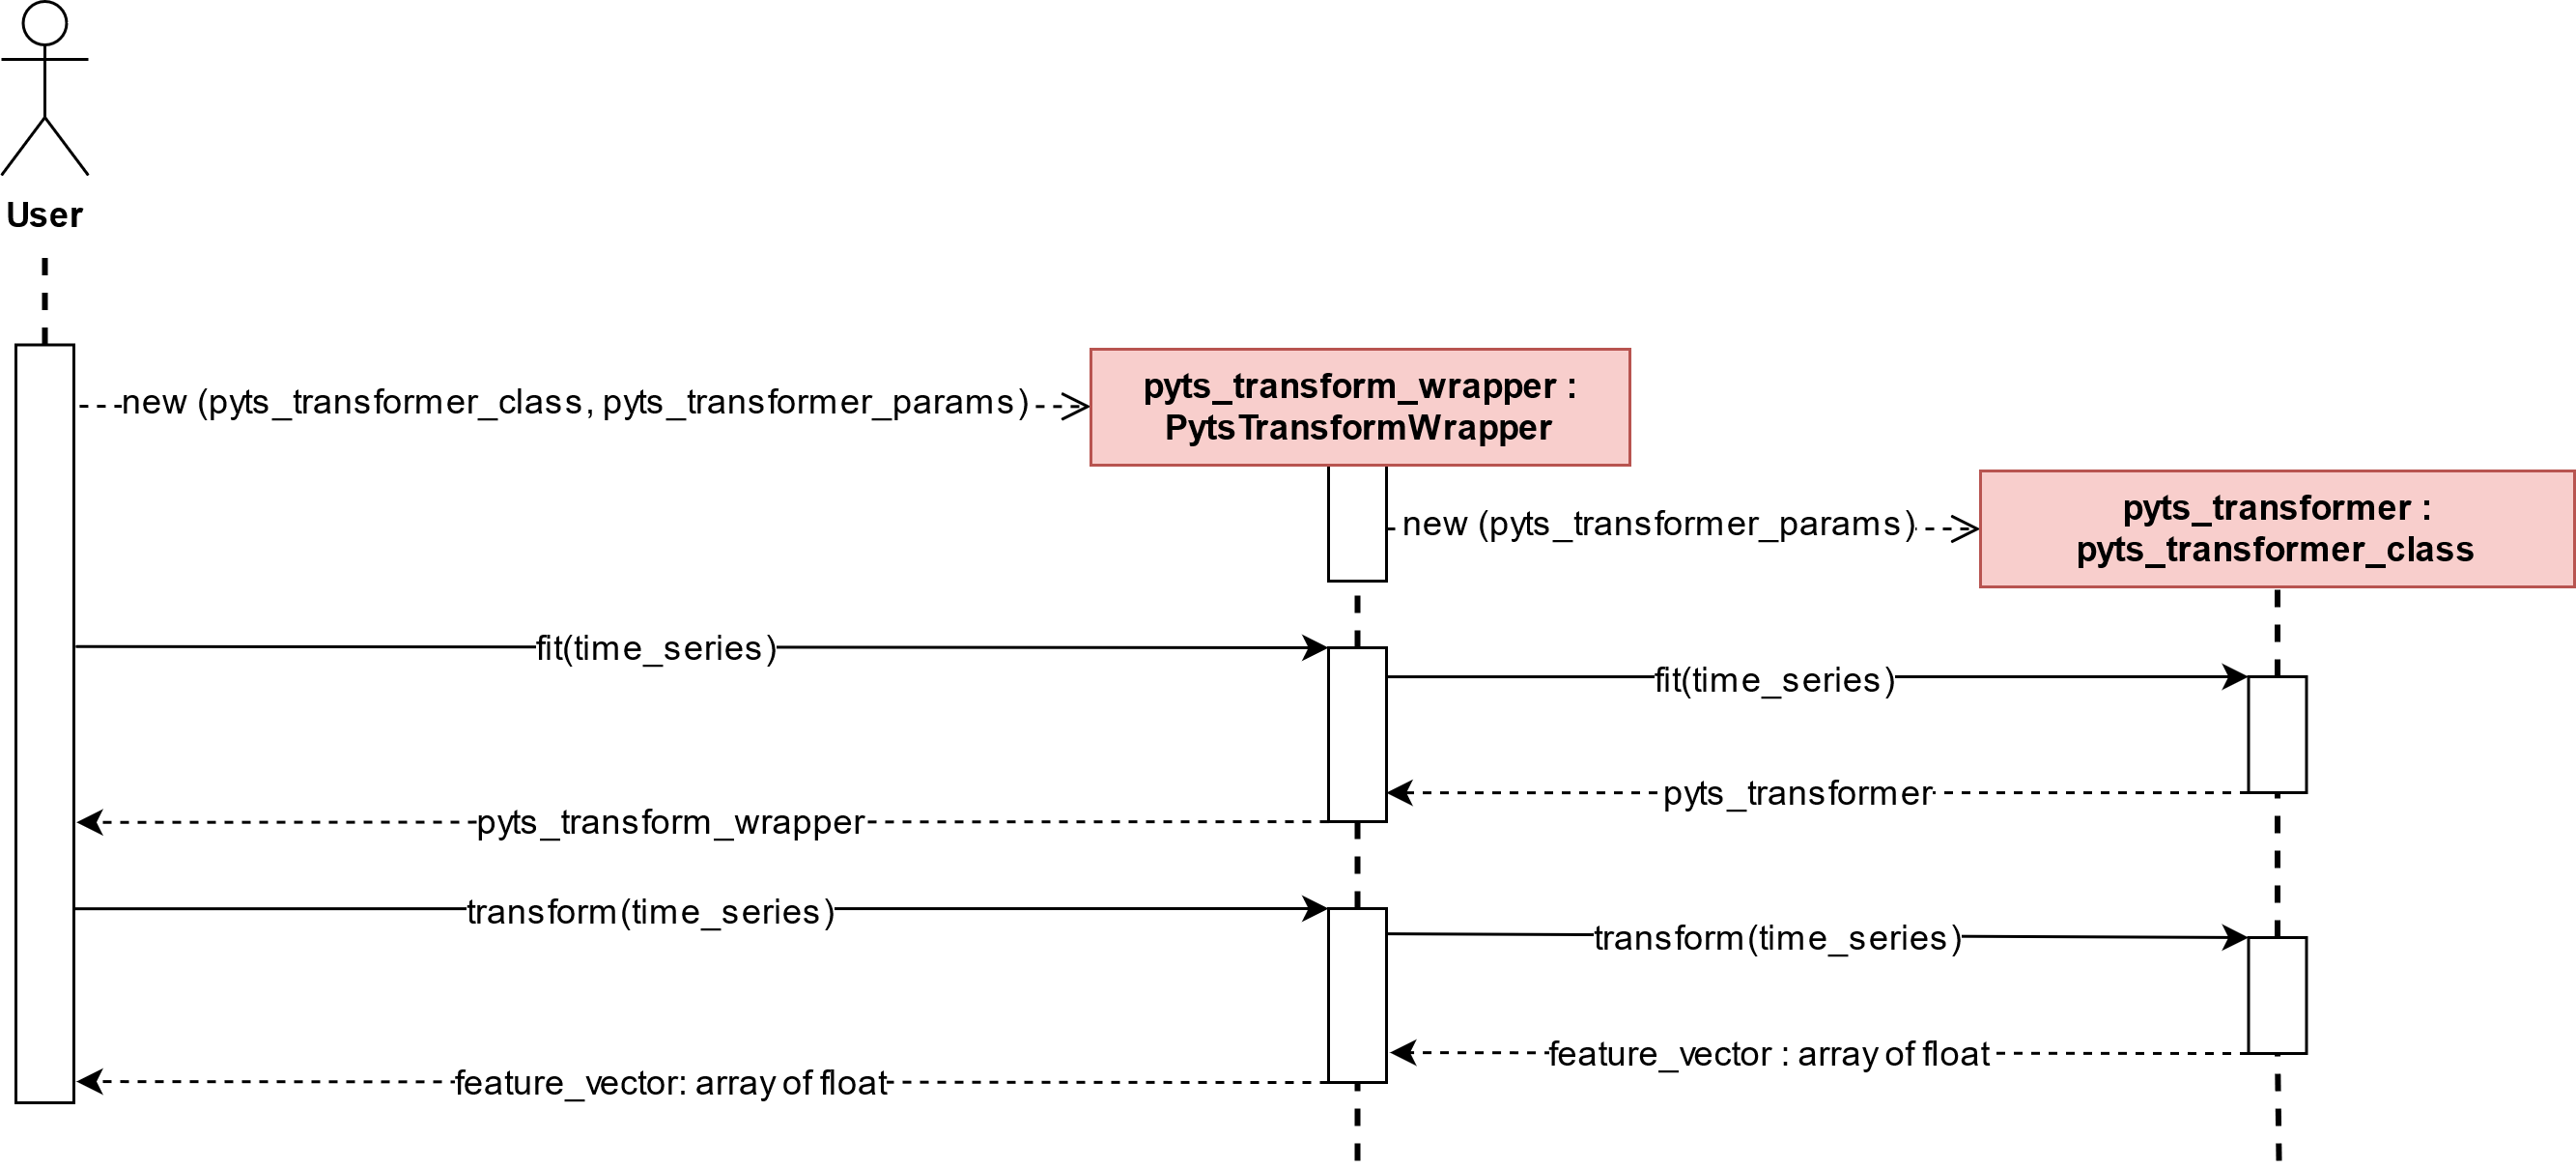
\includegraphics[width=\textwidth]{gfx/pyts_transform_sequence}
    \caption{Sequence Diagram of the PytsTransformWrapper class for fit and transform use-case.}
    \label{fig:tfe-pyts-transform-seq}
\end{figure}
\\
Figure \ref{fig:pyts-transform-wrapper-seq} show the use case for the fit and the transform function call with the ROCKET, Bag of Patterns, and Shapelet Transform. To access all the methods of \textit{pyts.transformation} class, we first need to initialize the \textit{pyts.transformation} class. From the \textit{PytsTransformeWrapper} class we can directly call the ROCKET, Bag of Patterns, and Shapelet Transform method which all return model as an object. Then we use this model to fit our time series data and transform the data. After fitting the Bag of Patterns model with the dataset it will give word frequencies for each time series. The \textit {fit\_transform} method of Shapelet Transform method return the feature vectors.
\begin{figure}[ht]
    \centering
    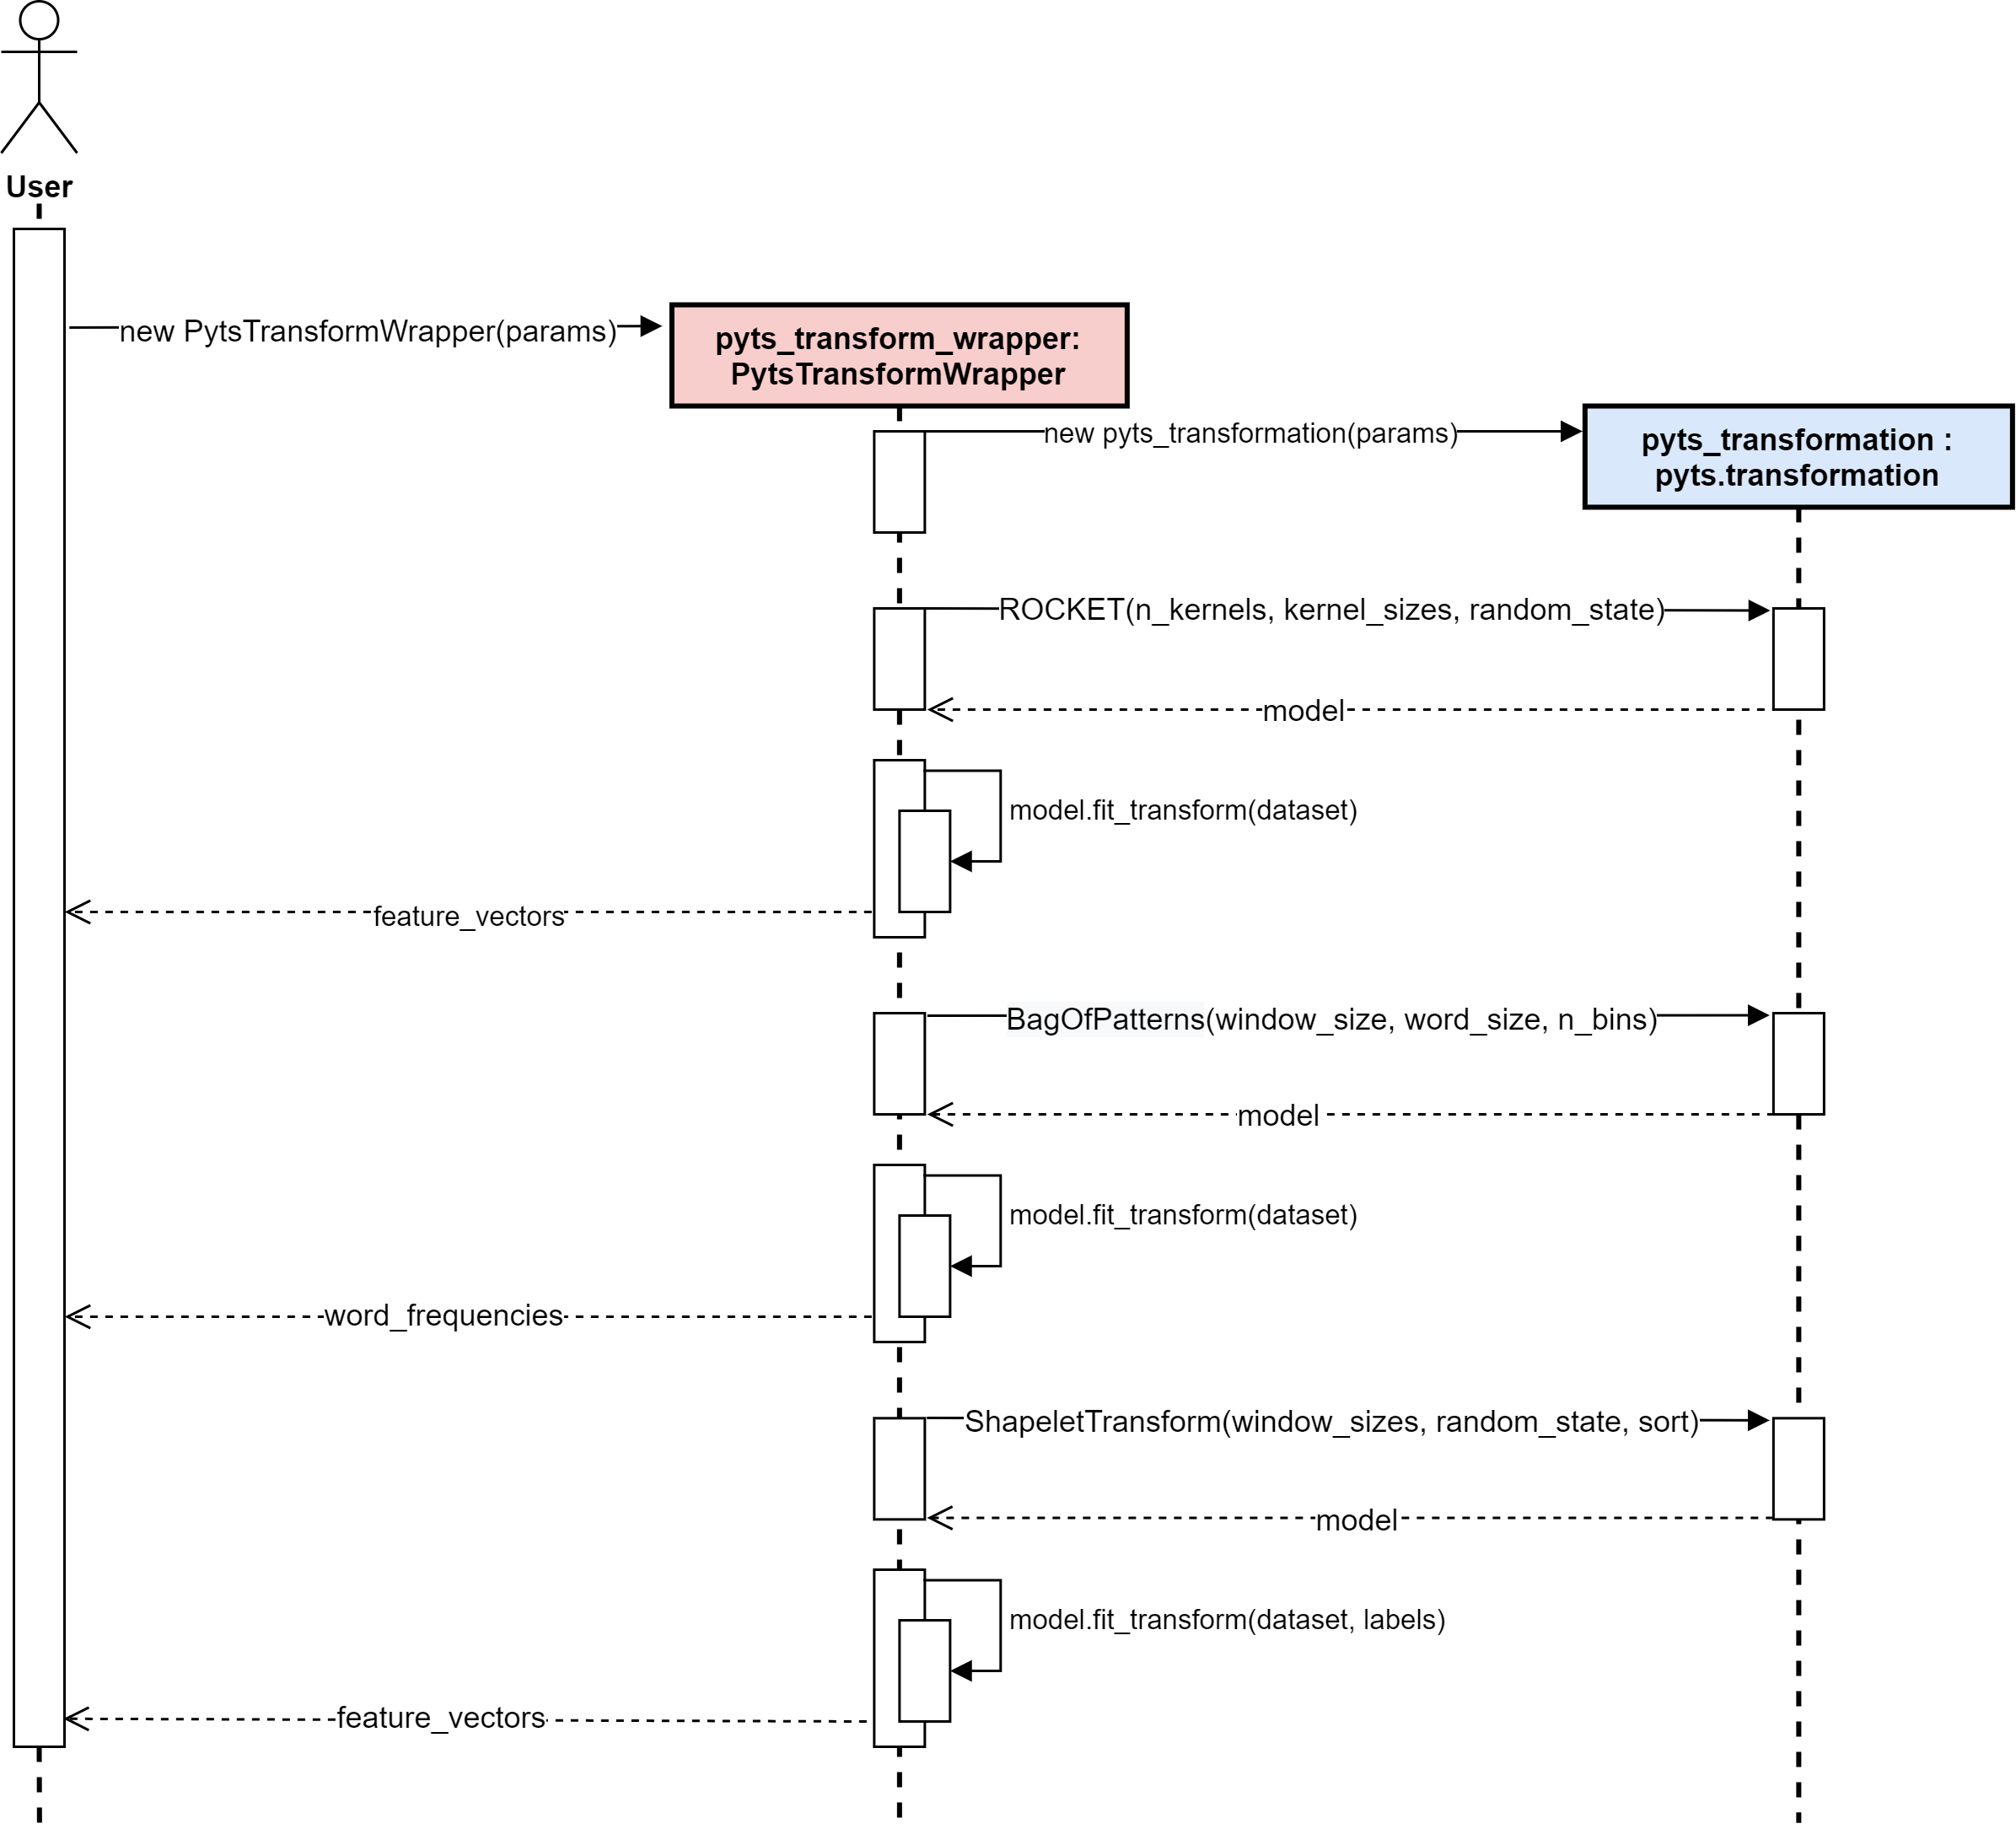
\includegraphics[width=\textwidth]{gfx/pyts_transform_wrapper-Sequence.png}
    \caption{Sequence Diagram of the PytsTransformWrapper class with ROCKET, BOP, and Shapelet Transform for fit and transform use-case.}
    \label{fig:pyts-transform-wrapper-seq}
\end{figure}
\subsubsection*{TSFreshWrapper}
\vspace*{-10mm}\hfill{\fontfamily{phv}\normalsize\emph{Sanjay Gupta}}
\\
The \textit{TSFreshWrapper} is a wrapper for the \textit{tsfresh} \footnote{\href{https://pypi.org/project/tsfresh/}{https://pypi.org/project/tsfresh/}} Package. The \textit{tsfresh} stands for Time Series Feature extraction based on scalable hypothesis tests. The package contains many feature extraction methods and feature selection algorithms. In Figure \ref{fig:tsfresh-wrapper-seq}, we show the use case for the fit and the transform function call. To access all the classes related to feature engineering we need to first initialize the \textit{tsfresh} package. The \textit{tsfresh.feature\_extraction.feature\_calculators} module contains more than sixty features or methods that take time series data as input and calculate the values of the feature.
\begin{figure}[ht]
    \centering
    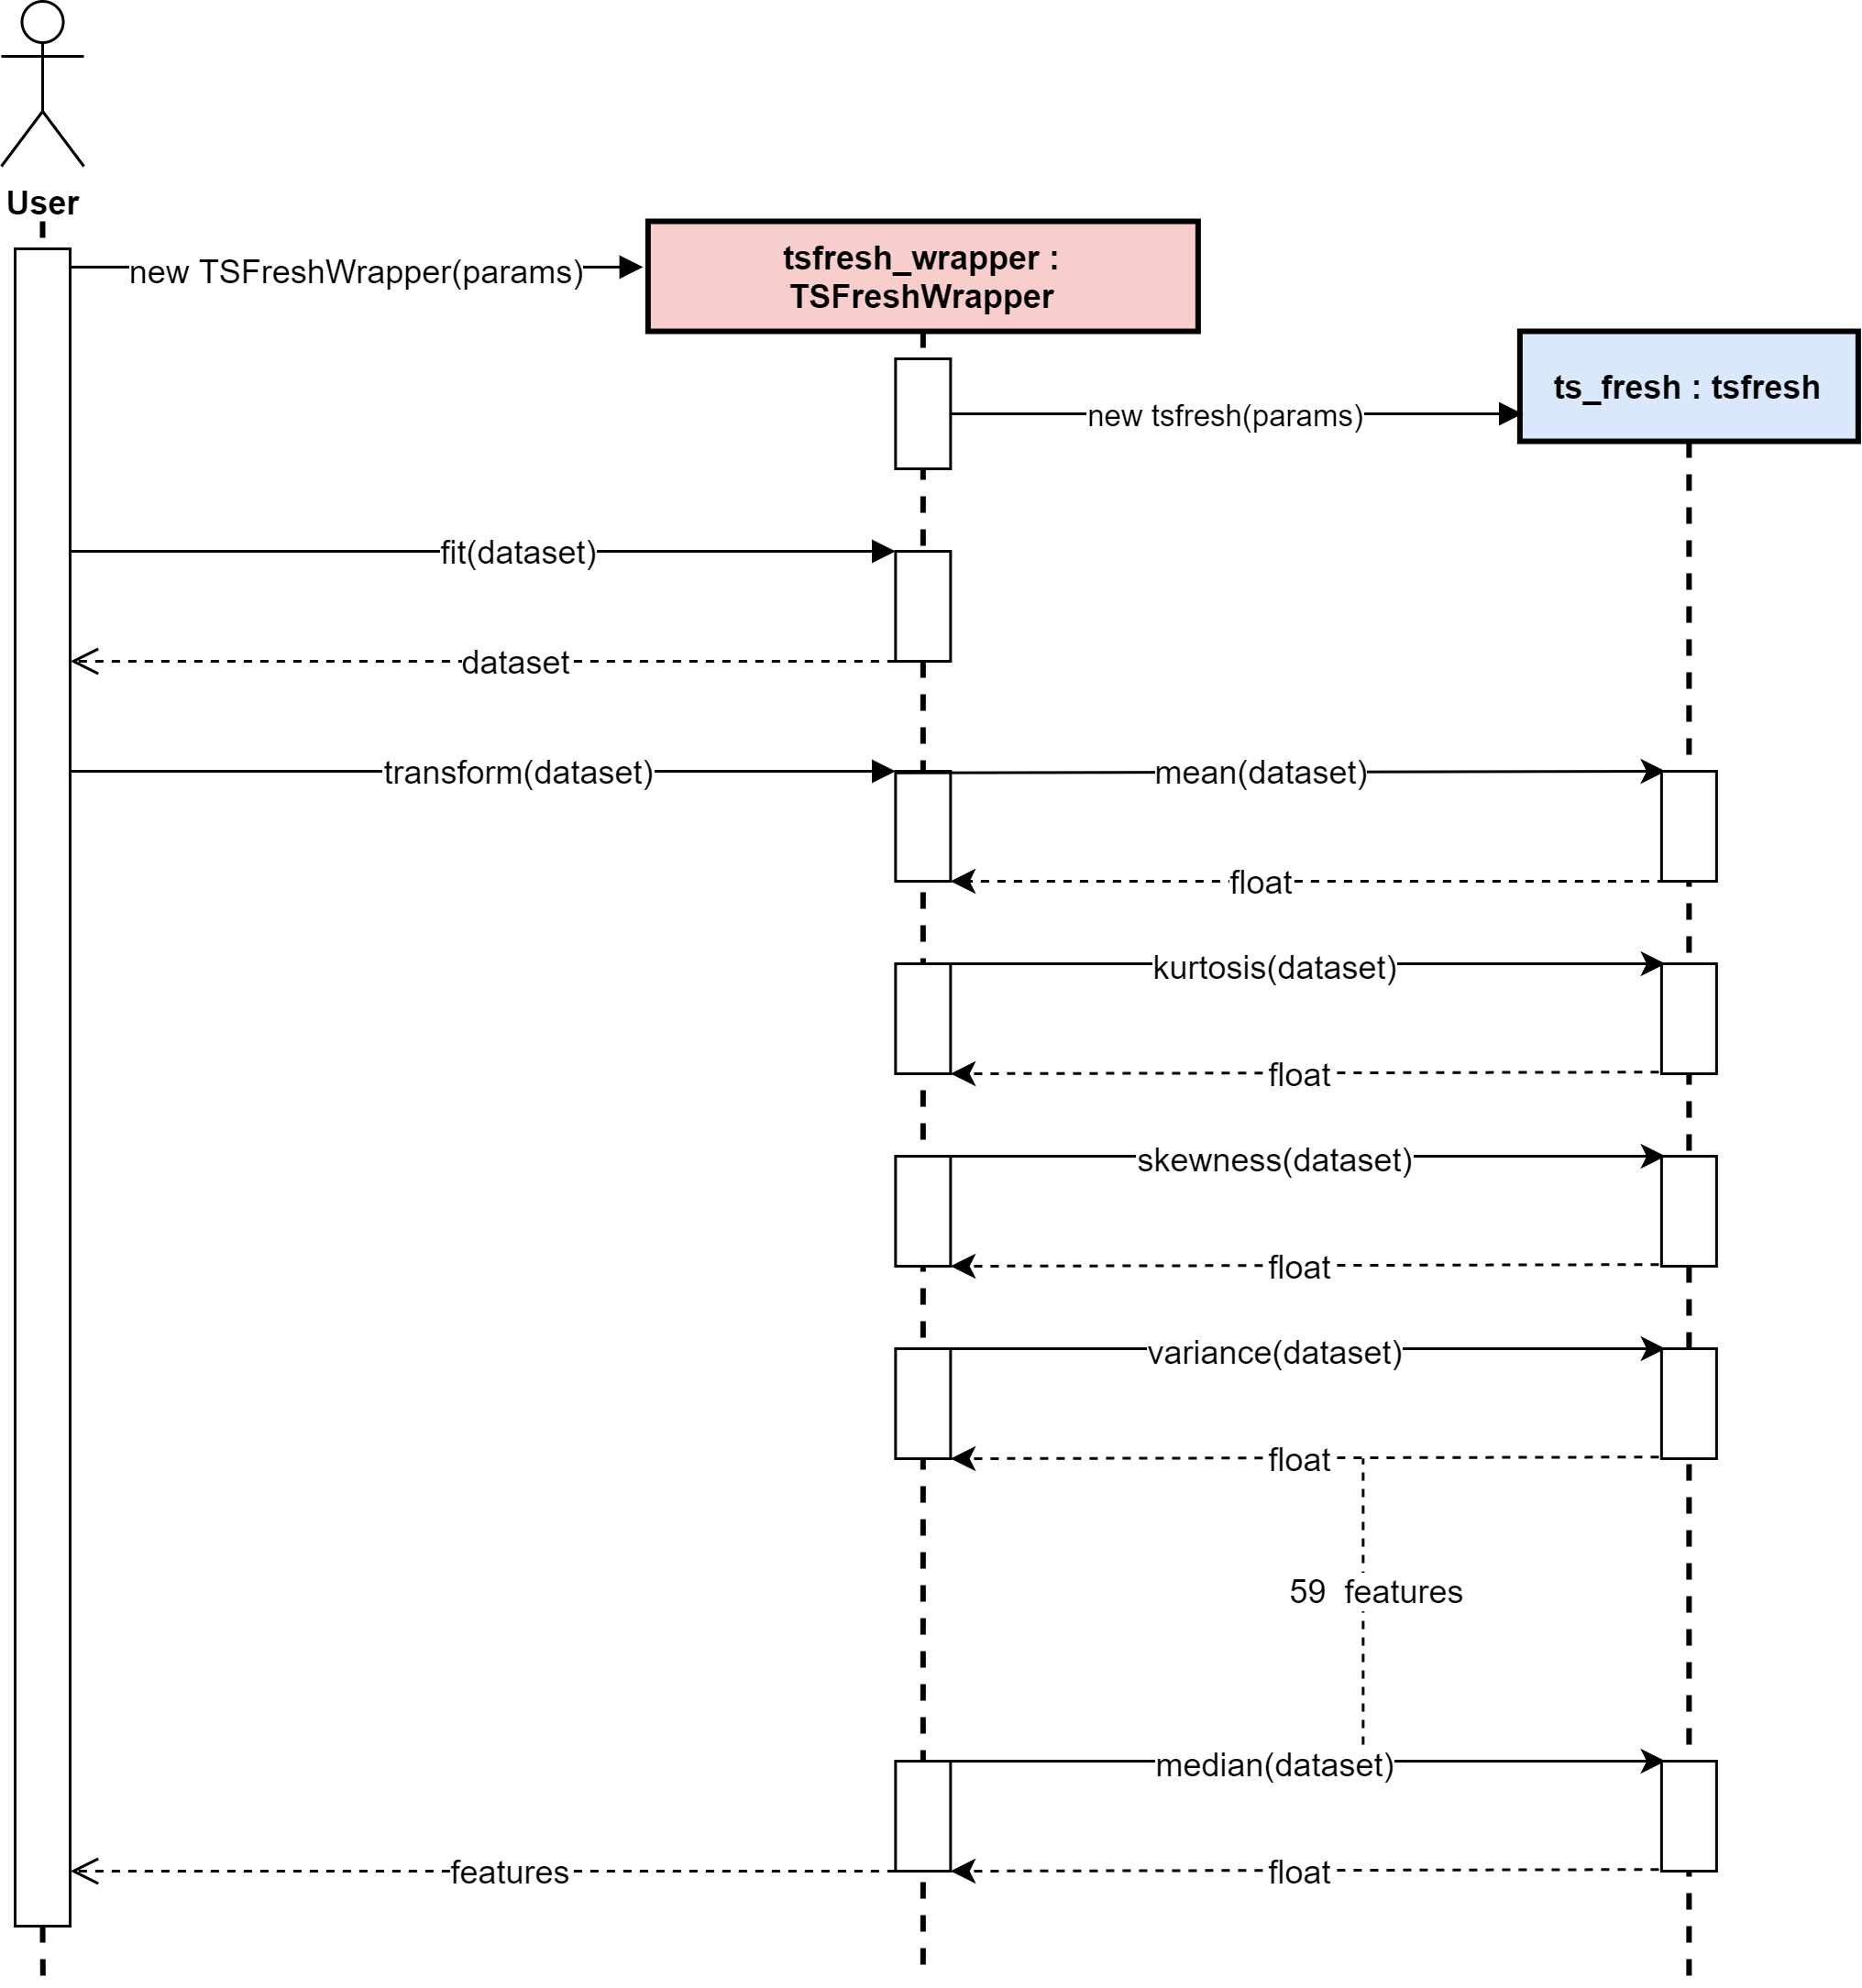
\includegraphics[width=\textwidth]{gfx/TSFreshWrapper-Sequence}
    \caption{Sequence Diagram of the TSFreshWrapper class for fit and transform use-case.}
    \label{fig:tsfresh-wrapper-seq}
\end{figure}
\subsubsection*{RNNAutoencoder}
\vspace*{-10mm}\hfill{\fontfamily{phv}\normalsize\emph{Sanjay Gupta}}
\\
The \textit{RNNAutoencoder} class use \textit{tensorflow} \footnote{\href{https://pypi.org/project/tensorflow/}{https://pypi.org/project/tensorflow/}} library to perform the RNN and Autoencoder functionality. Tensorflow is a open source software library for high-performance numerical computation. In Figure \ref{fig:rnn-seq}, we show the use case for the fit and the transform function call. To access all the classes which is required to implement RNN can be directly call in \textit{RNNAutoencoder} class after initialization of \textit{tensorflow} library. The \textit{RNNAutoencoder} class will return the feature vector as a output for the \textit{transform} call.
\begin{figure}[ht]
    \centering
    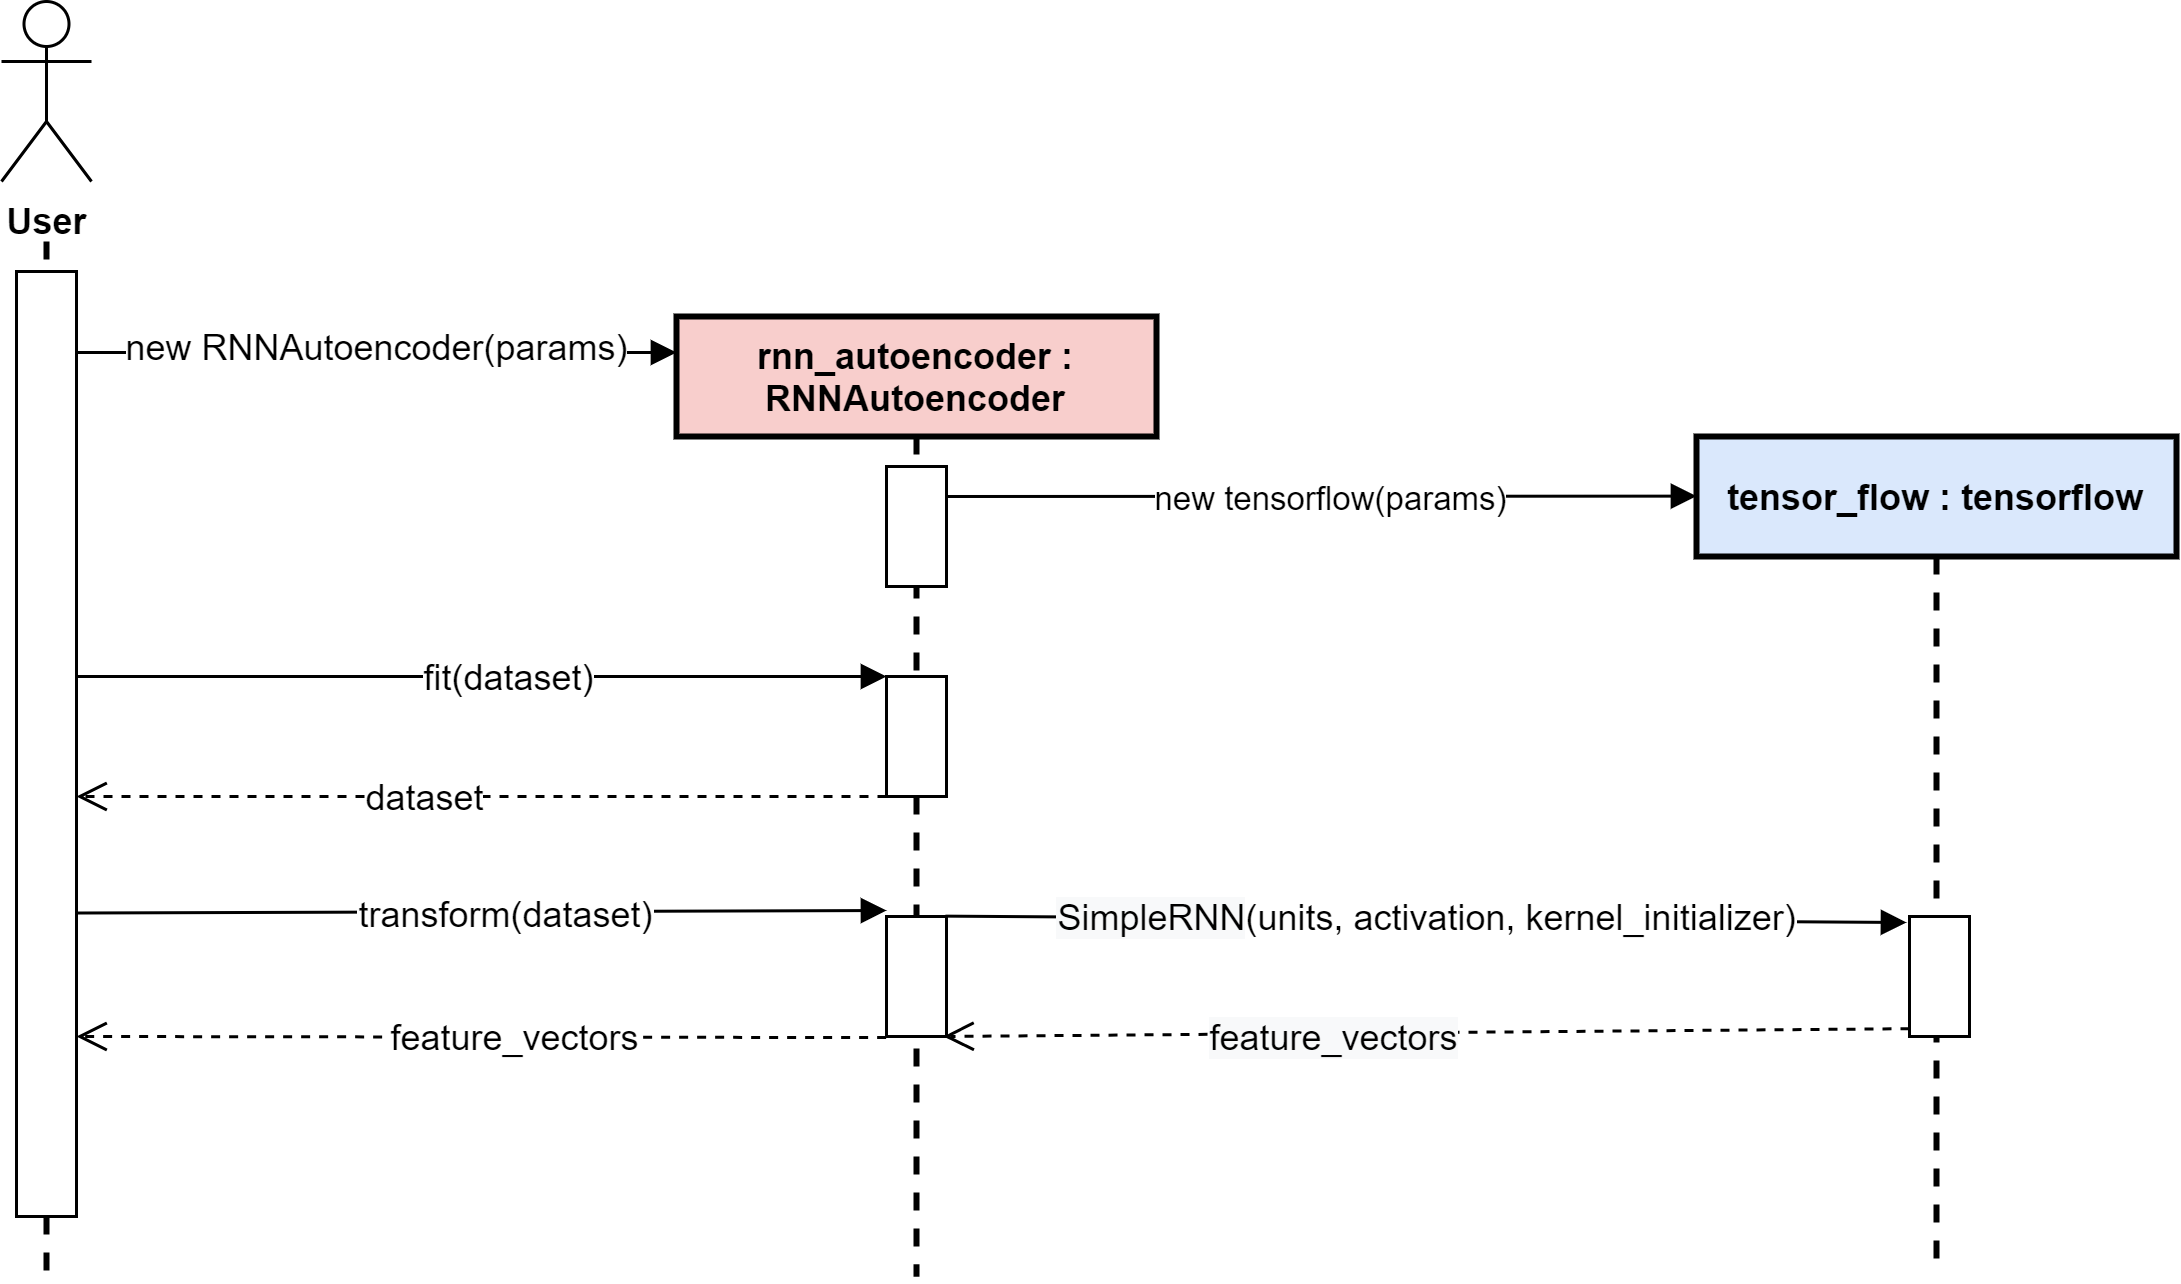
\includegraphics[width=\textwidth]{gfx/RNN-Sequence}
    \caption{Sequence Diagram of the RNN Autoencoder for fit and transform use-case.}
    \label{fig:rnn-seq}
\end{figure}
\subsubsection*{WindowingApproach}
\vspace*{-10mm}\hfill{\fontfamily{phv}\normalsize\emph{Sanjay Gupta}}
\\
The \textit{WindowingApproach} class use \textit{sklearn} \footnote{\href{https://pypi.org/project/scikit-learn/}{https://pypi.org/project/scikit-learn/}} module to perform the windowing transformation. The \textit{sklearn} is a python module for machine learning built on top of \textit{SciPy} \footnote{\href{https://www.scipy.org/}{https://www.scipy.org/}}. Using \textit{sklearn} library, we can perform classification, regression, clustering, dimensionality reduction, model selection, and preprocessing operation on datasets. In Figure \ref{fig:rnn-seq}, we show the use case for the fit and the transform function call. We can access all the classes and method of \textit{sklearn} module by initializing library in \textit{WindowingApproach} class. The \textit{WindowingApproach} class will return the window for each time series as a output for the \textit{transform} call.
\begin{figure}[ht]
    \centering
    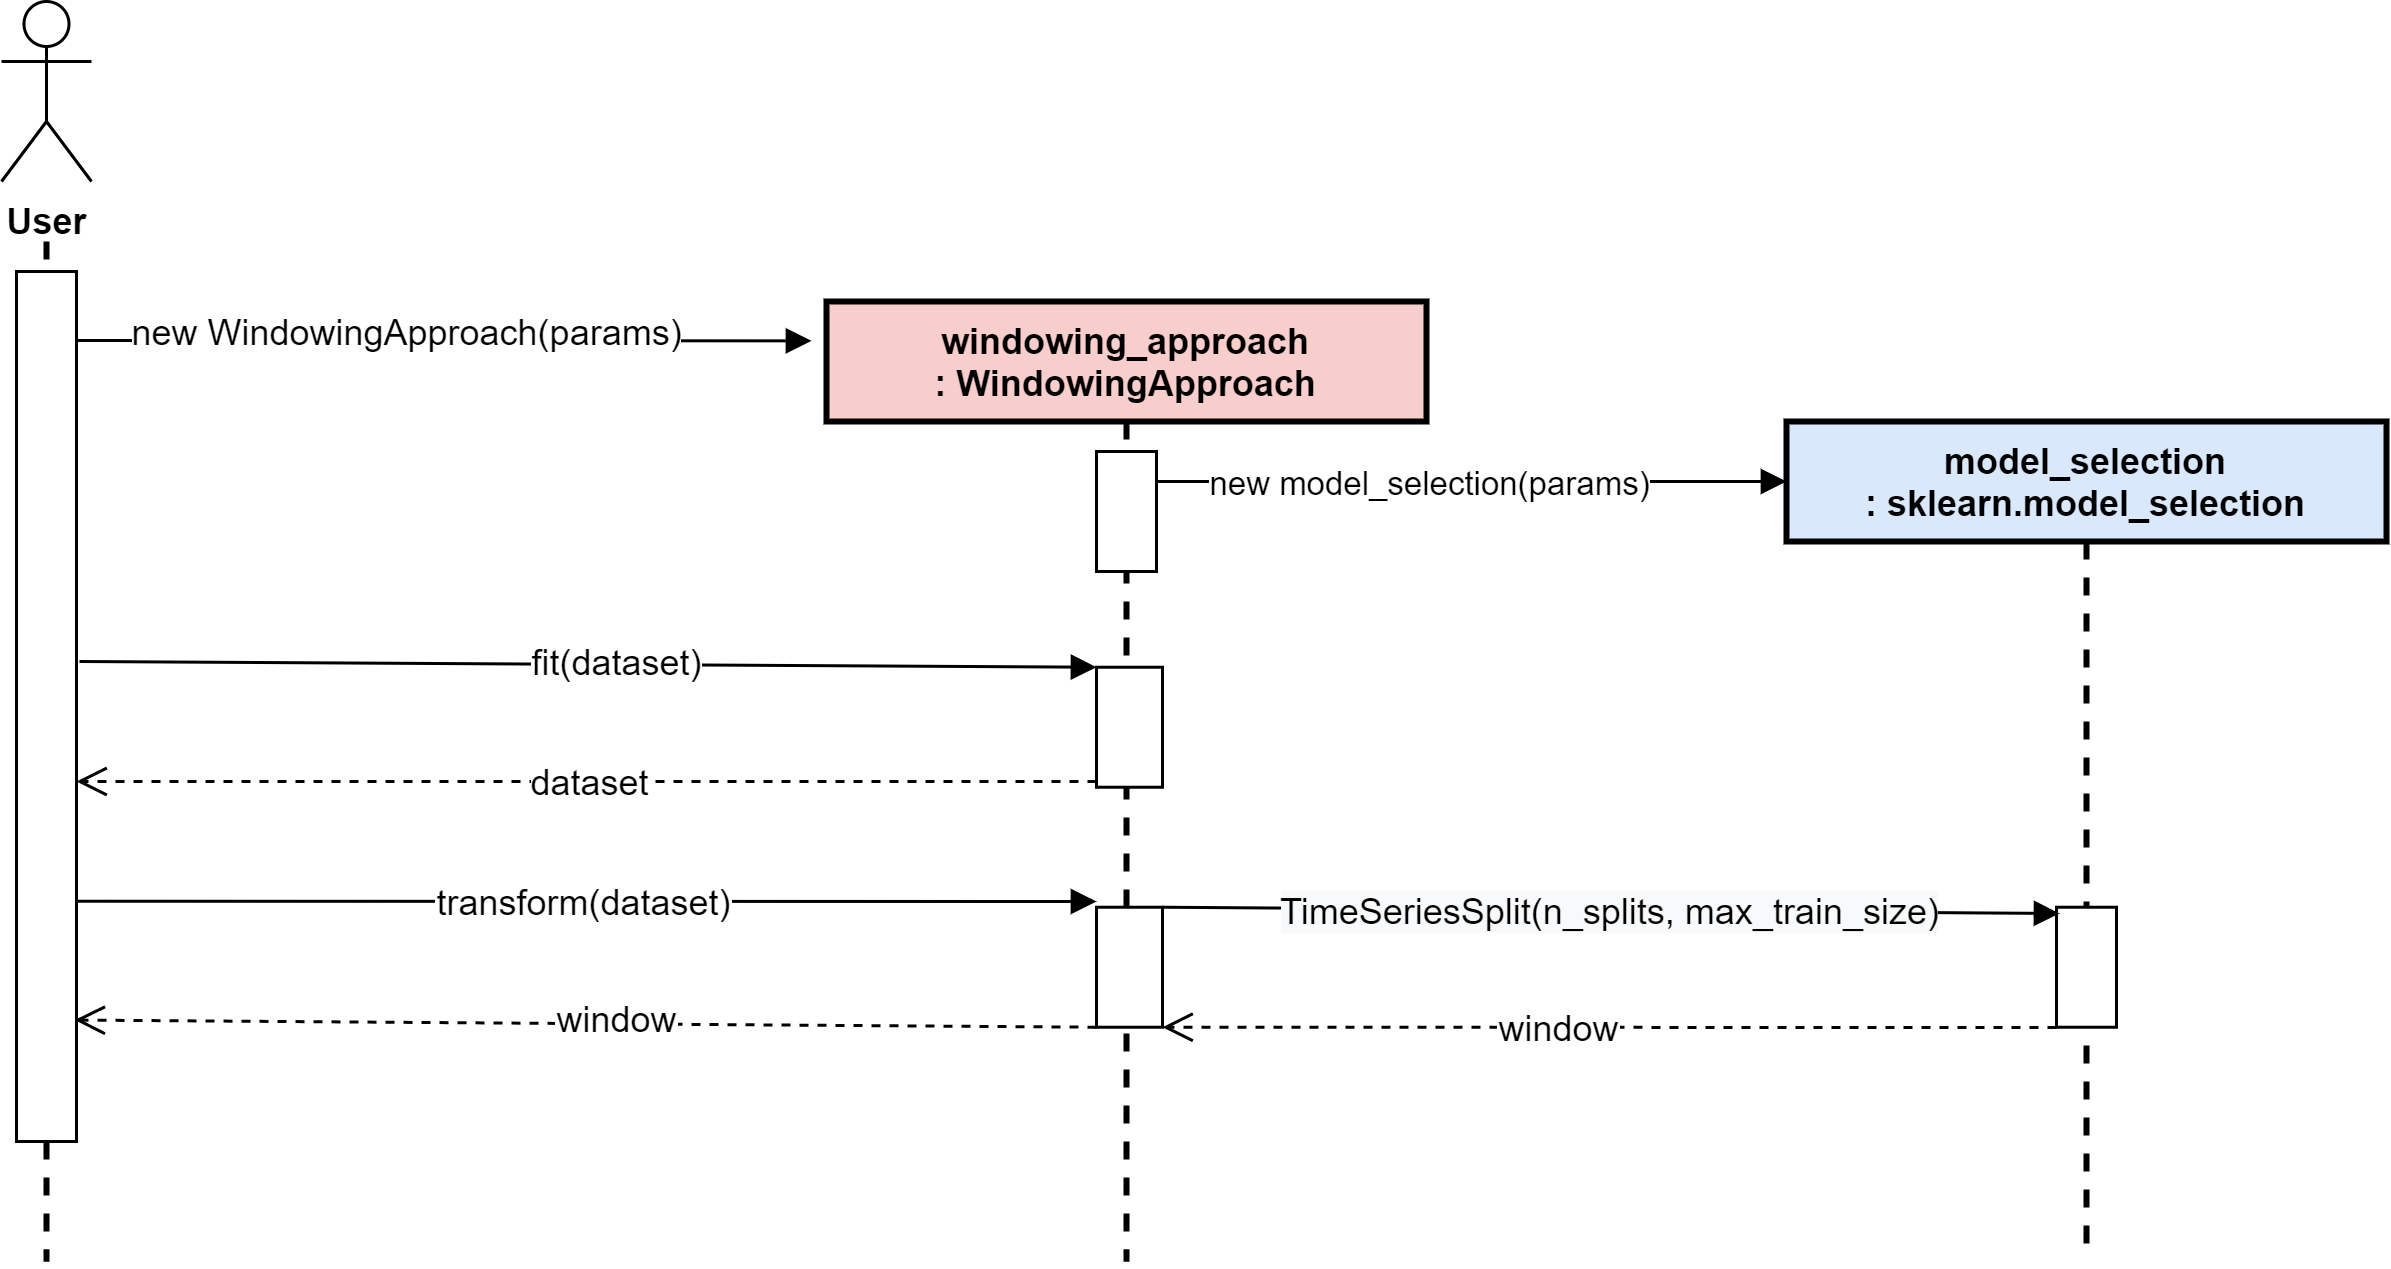
\includegraphics[width=\textwidth]{gfx/WindowApproach-Sequence}
    \caption{Sequence Diagram of the Windowing Approach for fit and transform use-case.}
    \label{fig:window-seq}
\end{figure}

\newpage
\section{Health Index Estimation}
\vspace*{-15mm}\hfill{\fontfamily{phv}\normalsize\emph{Selami Hoxha}}
\label{sec:system_design:health_index}

In this section the design for the health index estimation module of the framework is presented, starting with the class diagram and then
presenting sequence diagrams for the approaches that will be implemented.

\subsection*{Class diagram}
The class diagram of health index builds on the general class diagram. It extends the general class diagram by extending the HealthIndexEstimator abstract class.
In this module three approaches are presented with three purple box classes. The approaches use make use of different libraries like scikit-learn, tensorflow and scipy as shown
in the figure \ref{fig:class_hie}. In health index estimation also a Transformer abstract class from the general class diagram is used which will help with
feature extraction and other data transformation that are needed.
\begin{figure}[H]
    \centering
    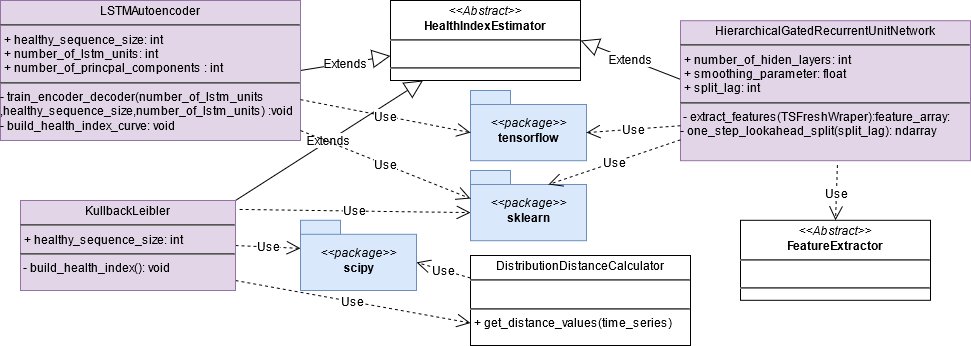
\includegraphics[width=\textwidth]{gfx/Interfaces-HIE.png}
    \caption{Class diagram for health index estimation module}
    \label{fig:class_hie}
\end{figure}

\subsection*{Sequence diagram}
The sequence diagrams try to show the flow of the approaches by showing the interactions between different classes. The sequence
diagrams for three approaches are presented in the figures \ref{fig:sequence_lstm}, \ref{fig:sequence_hgrun} and \ref{fig:sequence_KLD}.

\begin{figure}[H]
    \centering
    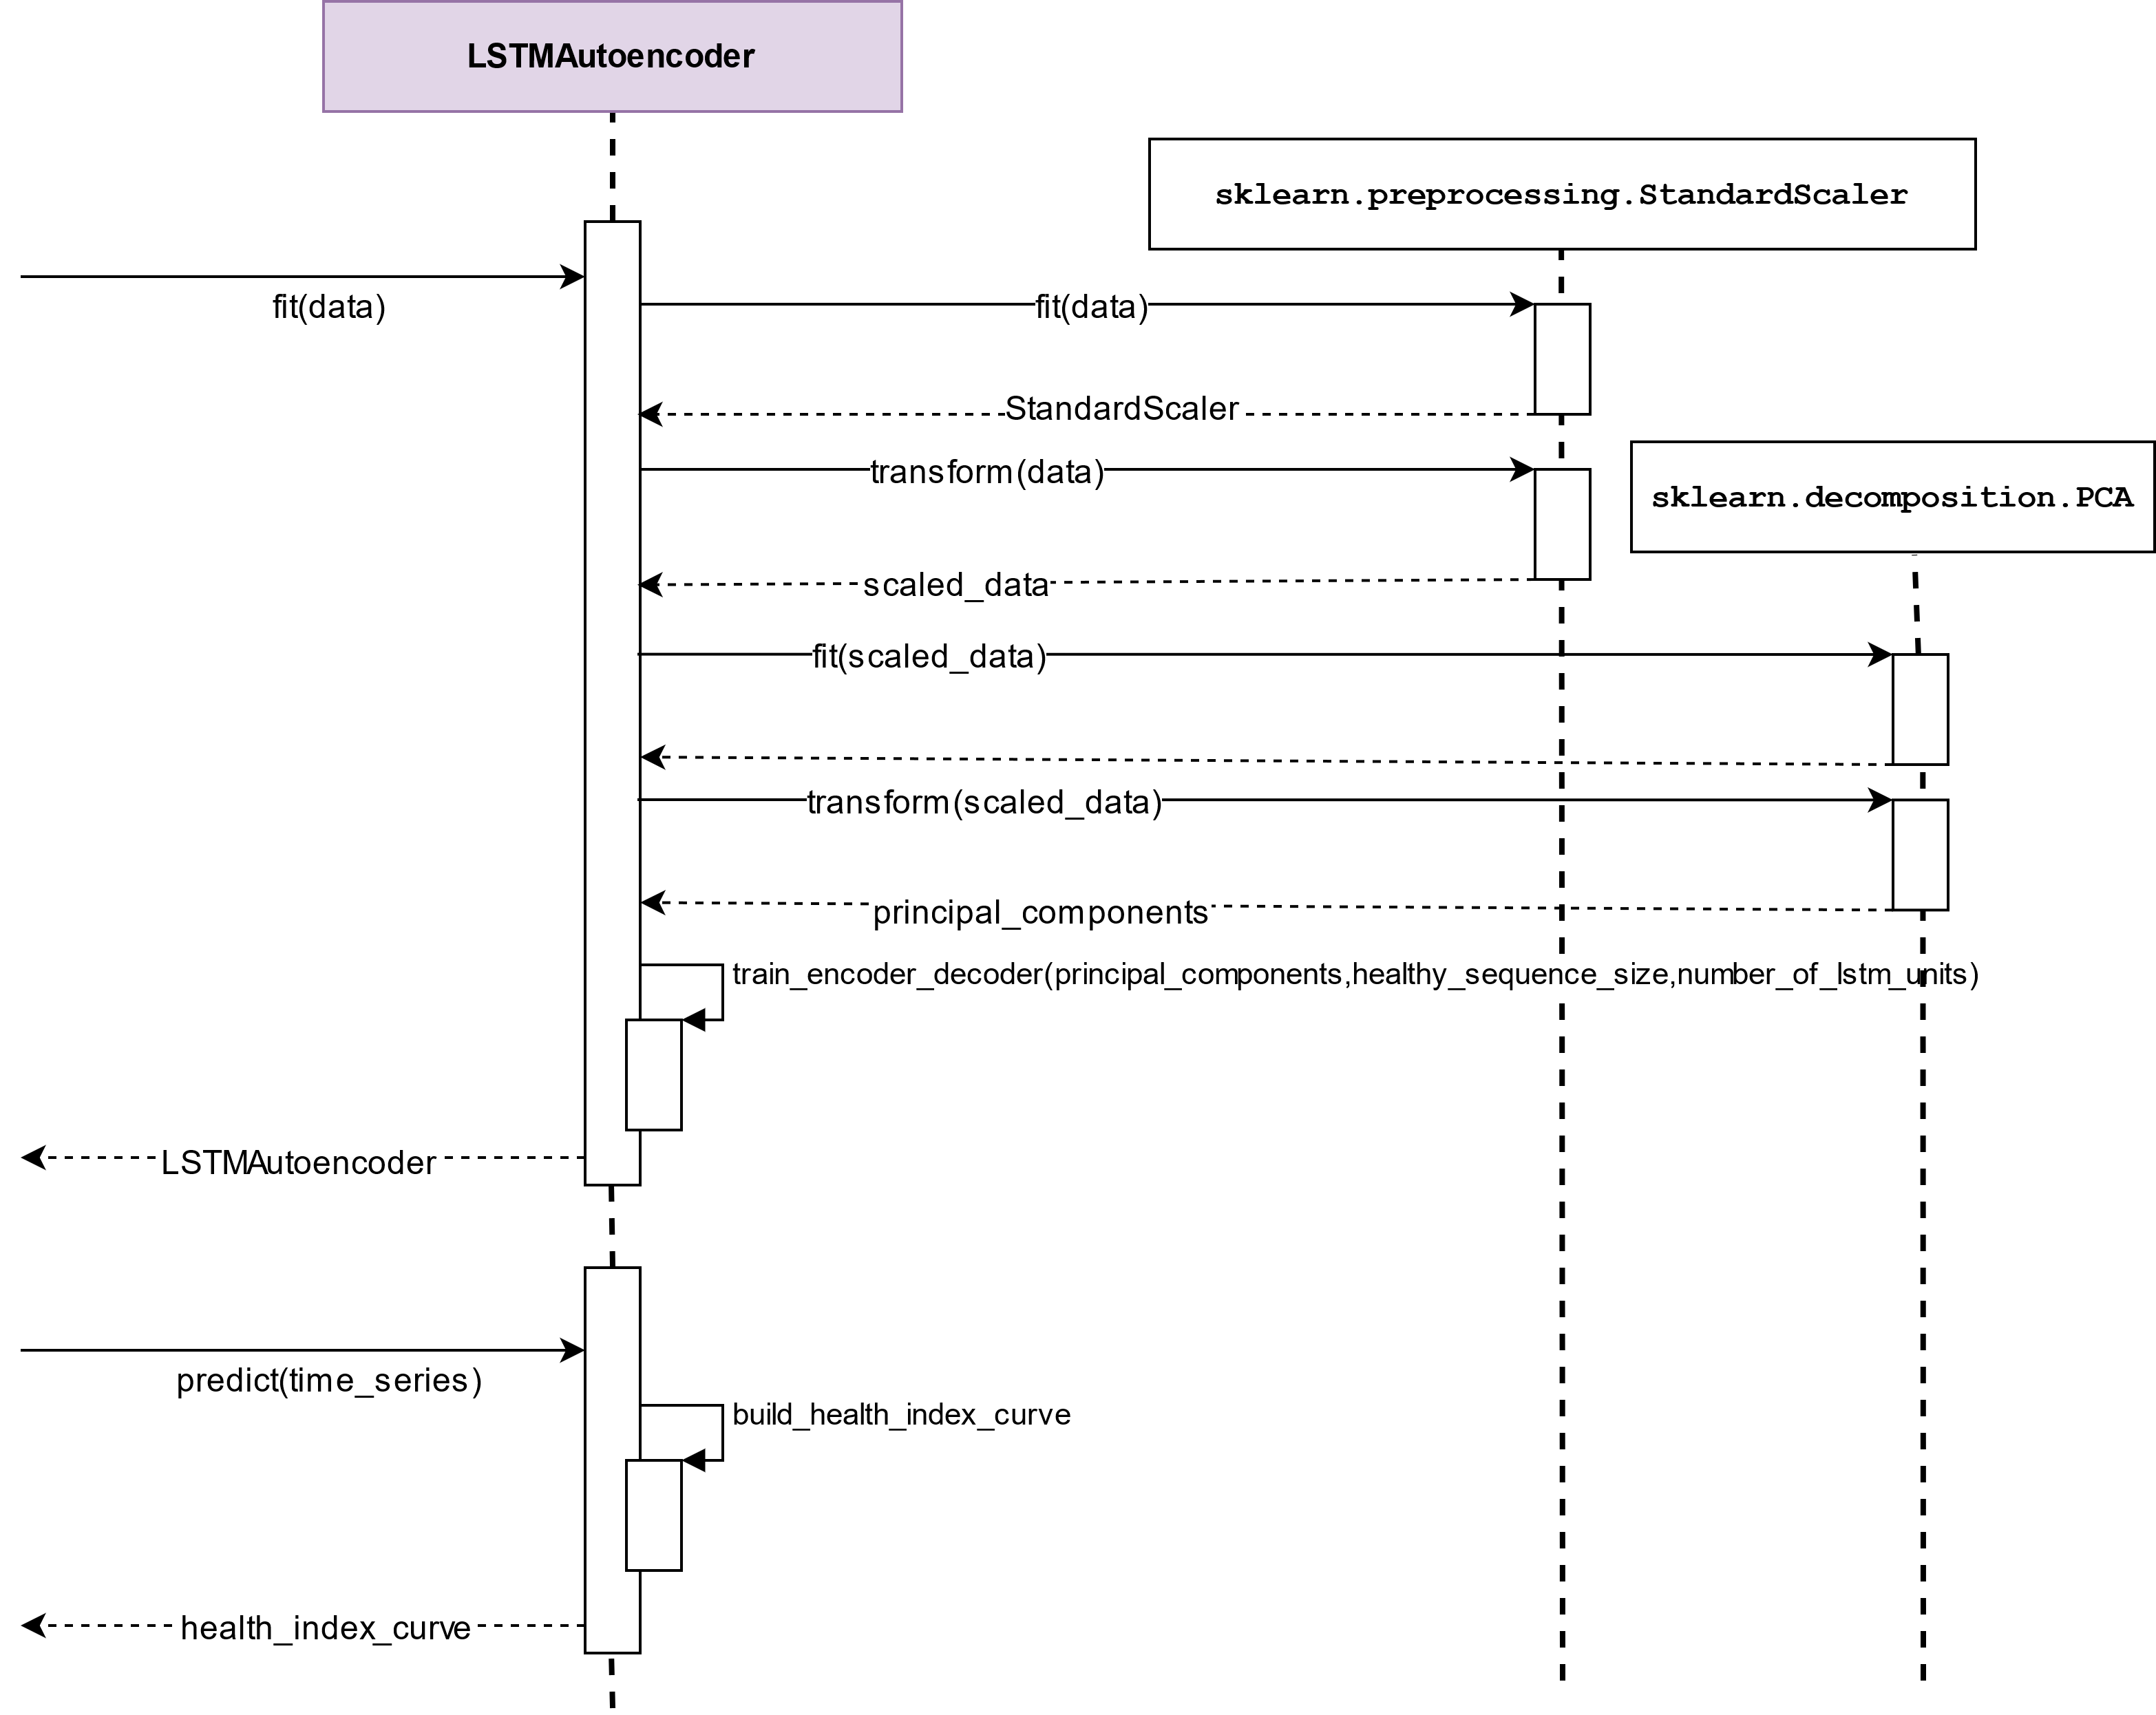
\includegraphics[width=\textwidth]{gfx/LSTMatuoencodersequencediagram.png}
    \caption{LSTM Encoder-Decoder HI estimation sequence diagram}
    \label{fig:sequence_lstm}
\end{figure}

\begin{figure}[H]
    \centering
    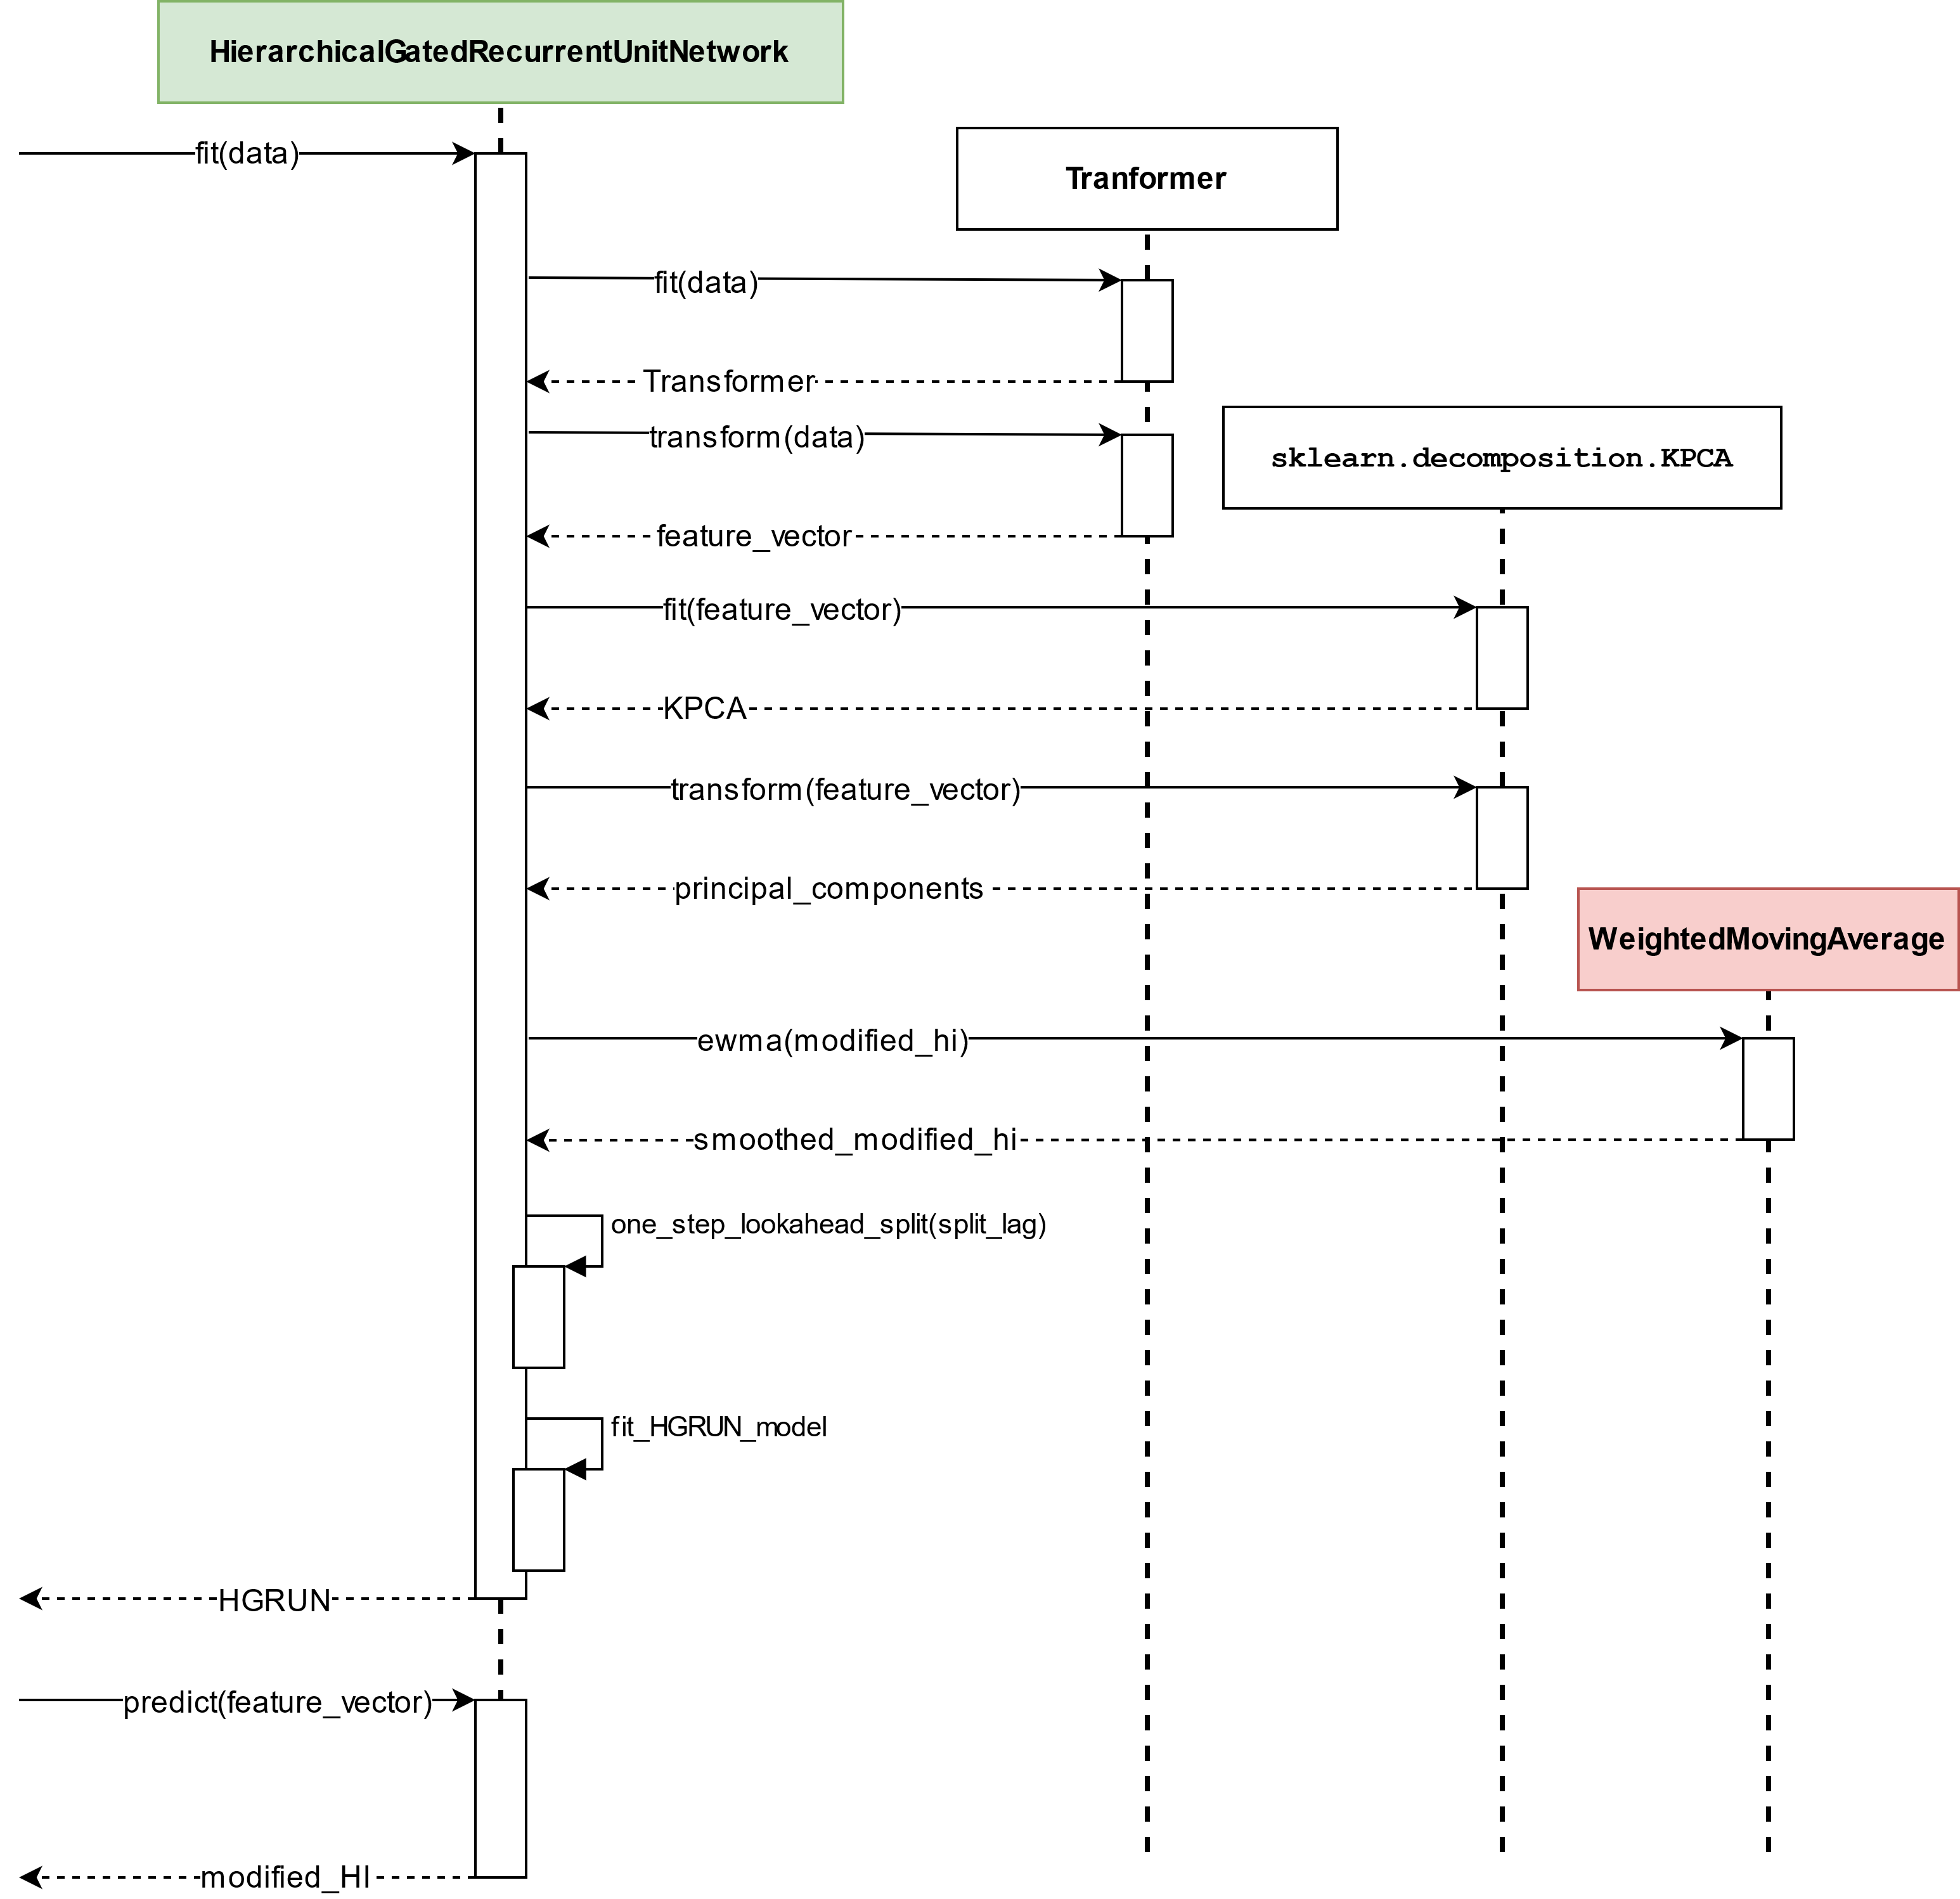
\includegraphics[width=\textwidth]{gfx/HGRUNsequencediagram.png}
    \caption{Hierarchical Gated Recurrent Unit Network HI estimation sequence diagram}
    \label{fig:sequence_hgrun}
\end{figure}

\begin{figure}[H]
    \centering
    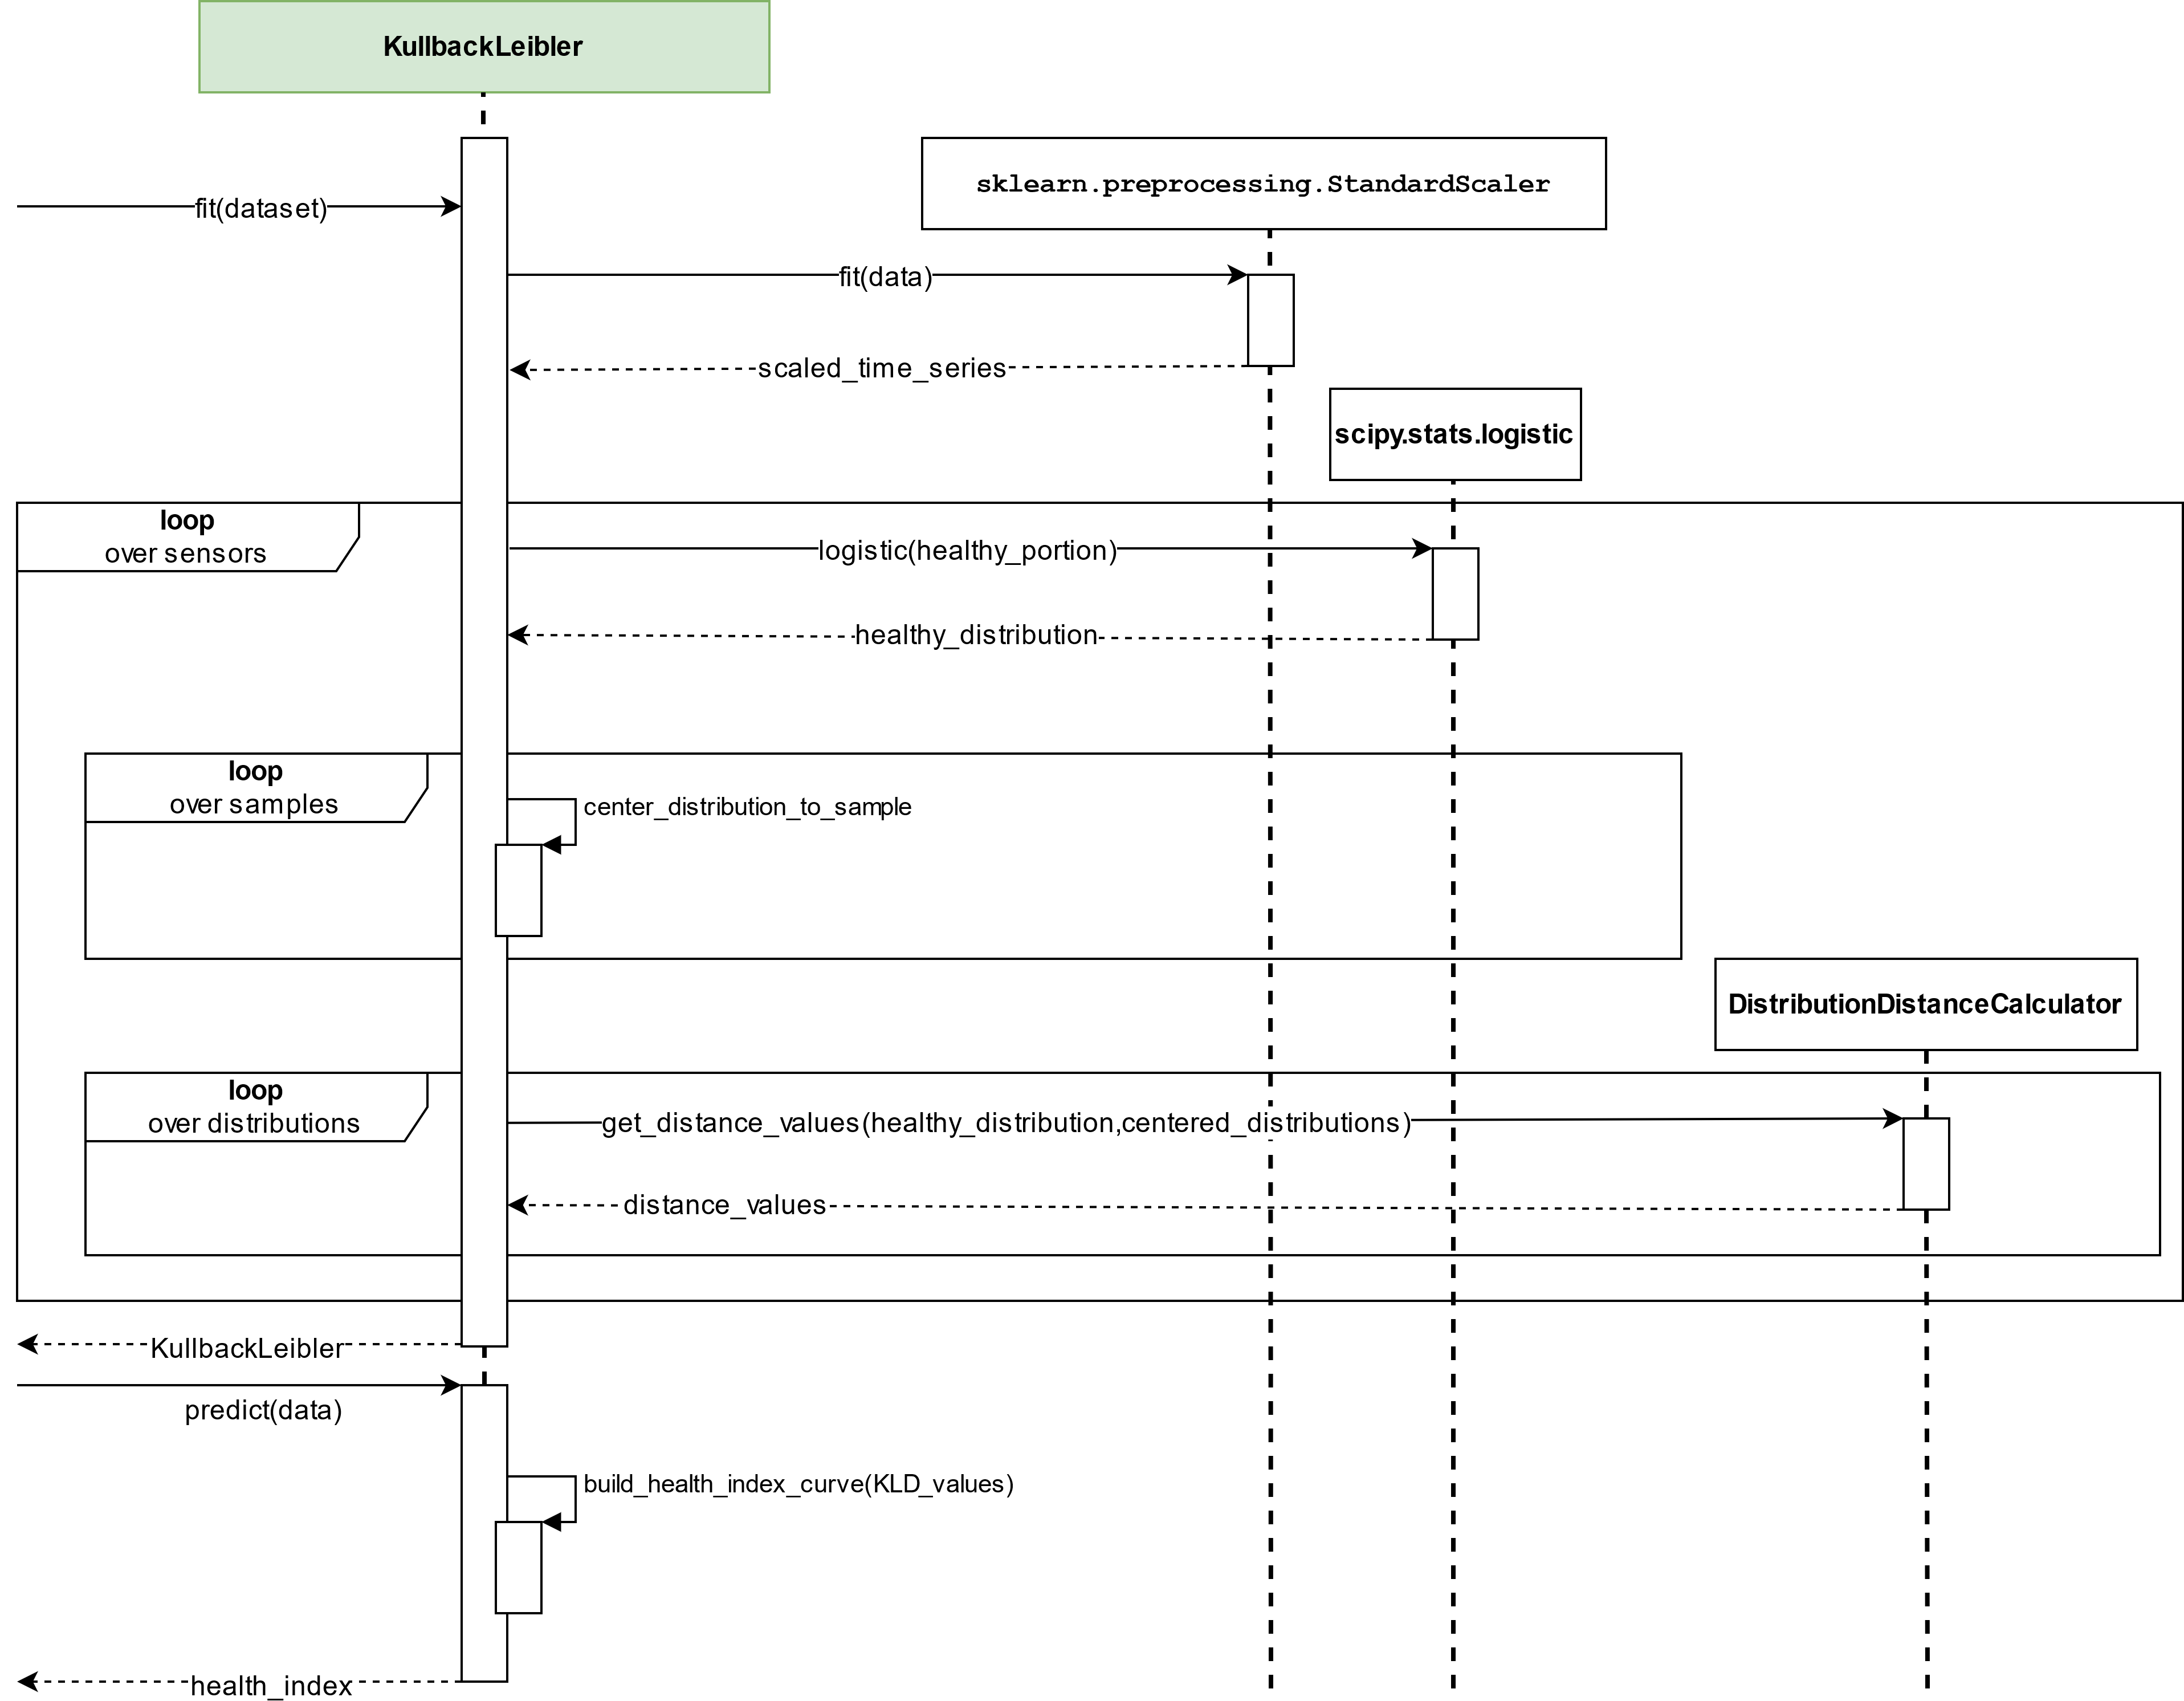
\includegraphics[width=\textwidth]{gfx/Kullbacksequencediagram.png}
    \caption{Kullback-Leibler Diveregence HI estimation sequence diagram}
    \label{fig:sequence_KLD}
\end{figure}

\section{Remaining Useful Lifetime Estimation}
\vspace*{-6.5mm}\hfill{\fontfamily{phv}\normalsize\emph{Vinay Kaundinya and Christopher Zinda}}

Different classes that are used in RUL estimation are described in this section, along with their parameters, methods and relationships.

\subsection*{Class diagram}
\vspace*{-12.5mm}\hfill{\fontfamily{phv}\normalsize\emph{Vinay Kaundinya and Christopher Zinda}}

The abstract class \textit{RemainingUsefulLifetimeEstimator} serves as a superclass for all RUL estimators and fixed pipelines. These will be described in an anti-clockwise manner in the following section.

The abstract class \textit{EnsembleApproach} in Figure \ref{fig:rul_class} acts as a superclass for all RUL approaches that consist of multiple elements of the same type. These elements are trained independently and when predicting the RUL, the individual predictions are aggregated to obtain a single prediction. One example of an ensemble approach is the \textit{MultipleClassifierApproach}. The \textit{MultipleClassifierApproach} saves the maximum failure horizon and holds multiple classifiers that are trained independently. The class \textit{EmbedRUL} resembles a pipeline out of four steps: \textit{WindowingApproach}, \textit{RNNAutoencoder}, \textit{HIEstimator}, \textit{RULEstimator}. Every pipeline step saves its configuration parameters that can also be set in the \textit{EmbedRUL} constructor. The \textit{transform} methods are specified to show the interconnection between the pipeline steps because the output of one step serves as an input to the next step. The abstract class \textit{CNN} in Figure \ref{fig:rul_class} acts as a superclass for all CNN approaches that allows user to choose only neural network model over the CNN approach that is proposed here. The abstract class \textit{SVR} then acts as a superclass for all SVR based approaches, which allows user to choose only SVR model over the Direct RUL approach which also extends an SVR model. The class \textit{LSTM} is nothing but a pipeline of calls to two normalizations \textit{MinMaxScaler} and \textit{StandardScaler} followed by different calls to methods in \textit{tf.keras.layers}.
\begin{figure}[H]
    \centering
    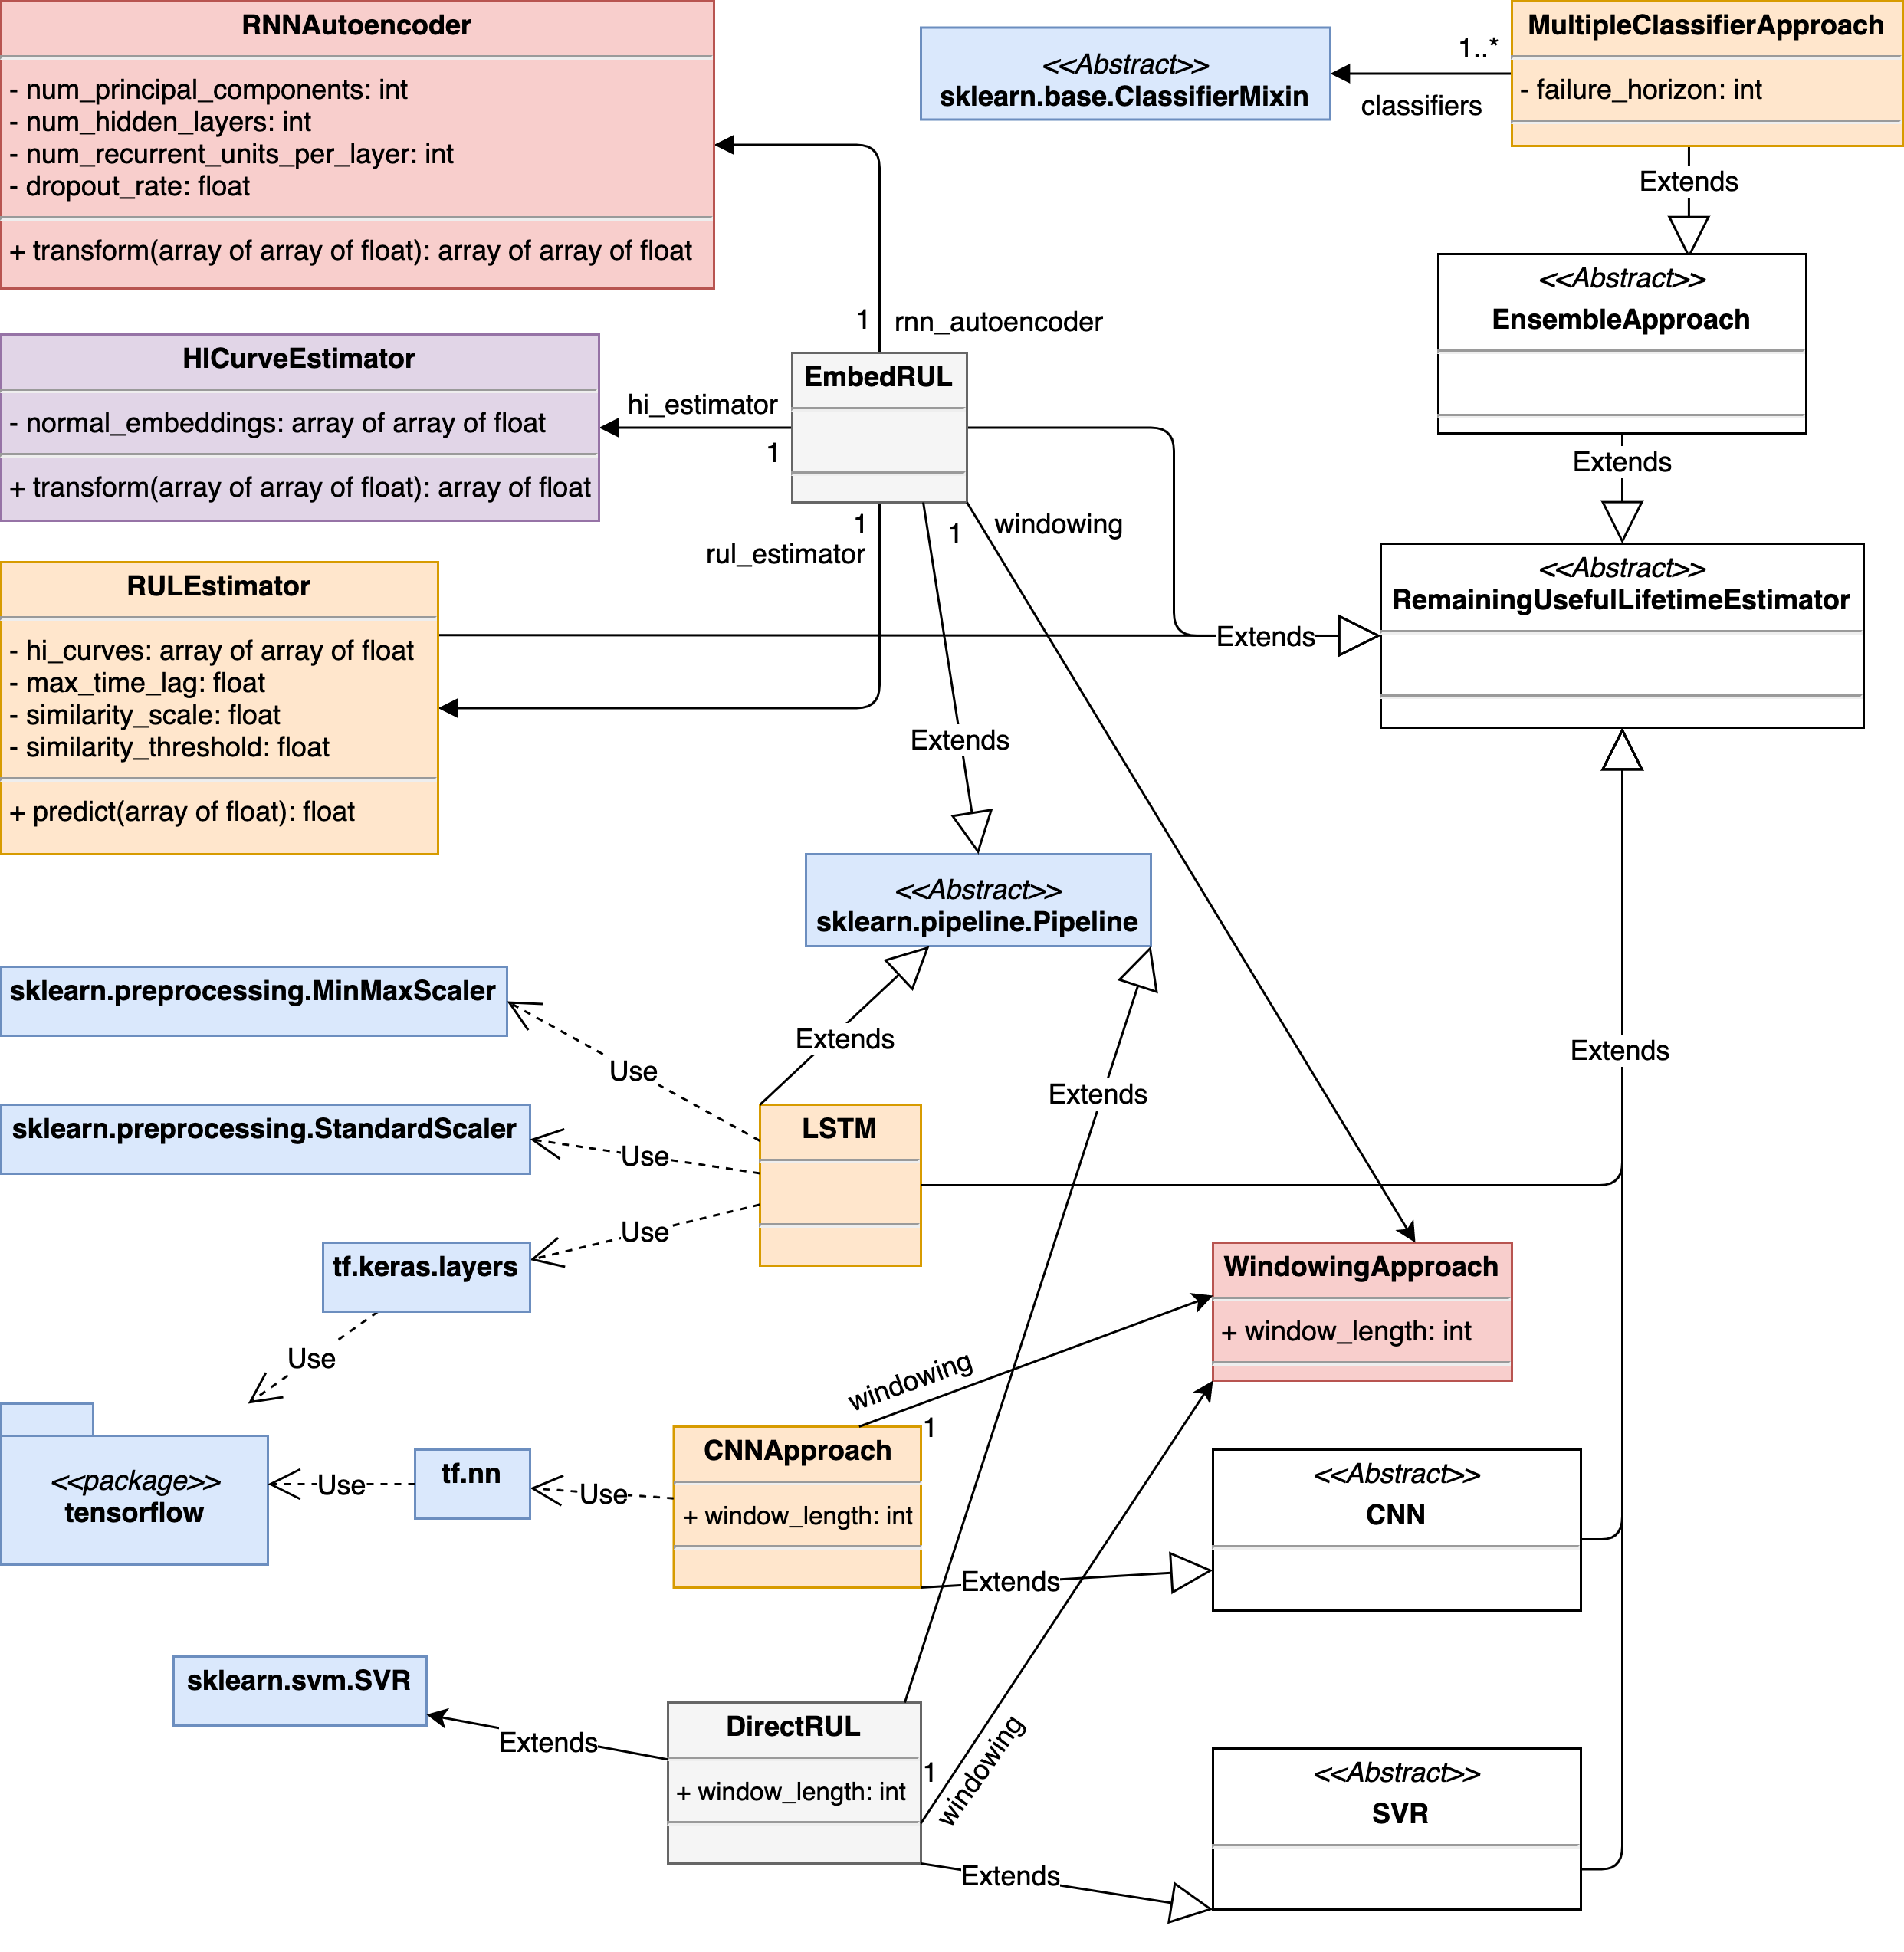
\includegraphics[width=\textwidth]{gfx/rul_class}
    \caption{Class diagram showing specific classes needed for Remaining Useful Lifetime Estimation.}
    \label{fig:rul_class}
\end{figure}

\subsection*{Sequence diagrams}
\vspace*{-12.5mm}\hfill{\fontfamily{phv}\normalsize\emph{Vinay Kaundinya and Christopher Zinda}}

Sequence diagrams for each of the RUL approaches are presented in the following section.

\subsubsection*{Multiple Classifier Approach}
\vspace*{-12.5mm}\hfill{\fontfamily{phv}\normalsize\emph{Christopher Zinda}}

The Multiple Classifier Approach is initialized with a parameter that defines the maximum failure horizon. As shown in Figure \ref{fig:rul_seq_multiple_classifier}, the array of \textit{ClassifierMixin} is initialized in the constructor. In the \textit{fit} method, the dataset is first prepared with annotations of different failure horizons. Every classifier is then fitted on one of the prepared datasets. In the \textit{predict} method we can then evaluate all classifiers and aggregate their predictions as described in the topic study document.
\begin{figure}[H]
    \centering
    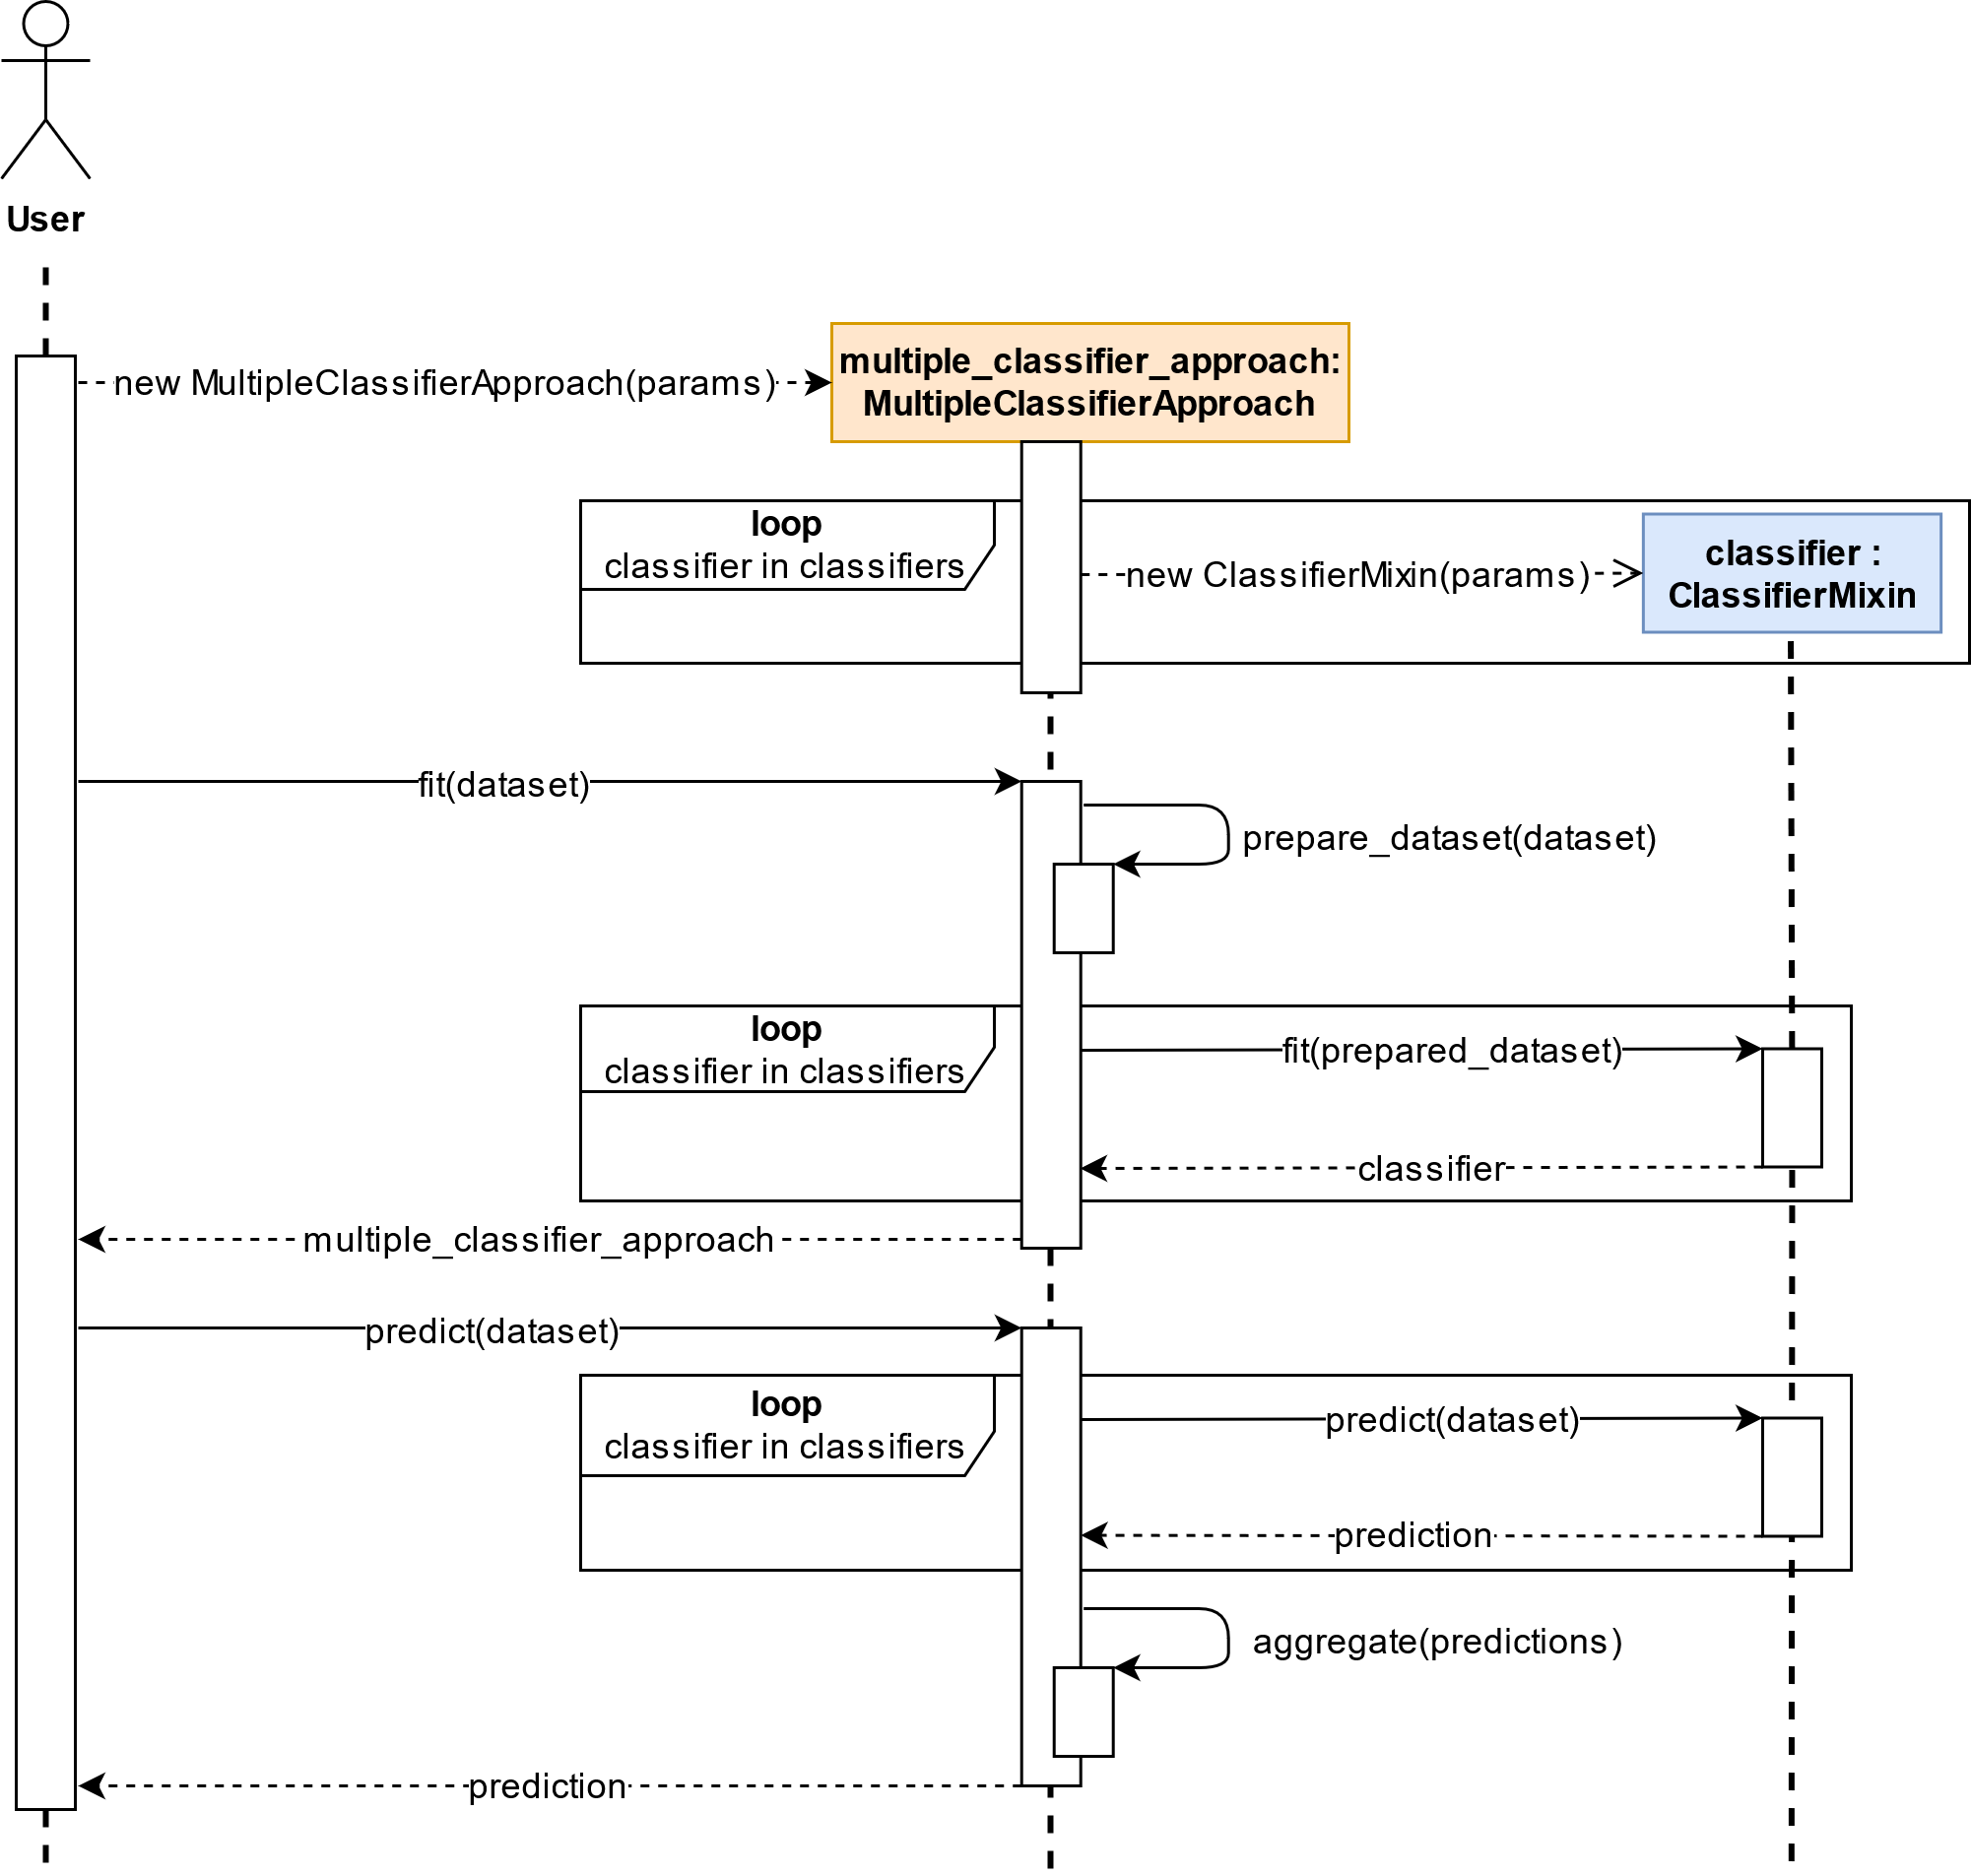
\includegraphics[width=\textwidth]{gfx/rul_seq_multiple_classifier}
    \caption{Sequence diagram of the Multiple Classifier Approach for fit and predict use case.}
    \label{fig:rul_seq_multiple_classifier}
\end{figure}

\subsubsection*{Embed RUL}
\vspace*{-12.5mm}\hfill{\fontfamily{phv}\normalsize\emph{Christopher Zinda}}

As shown in Figure \ref{fig:rul_seq_embed_rul}, the \textit{EmbedRUL} class first initializes the four pipeline steps \textit{WindowingApproach}, \textit{RNNAutoencoder}, \textit{HIEstimator} and \textit{RULEstimator}. These four elements are then also fitted in the same order. The output of one step is passed to the next step as input. The same pipeline execution happens in the \textit{predict} method to finally generate a RUL prediction. Details on the operation of each individual fit and transform/predict method can be found in the topic study document.
\begin{figure}[H]
    \centering
    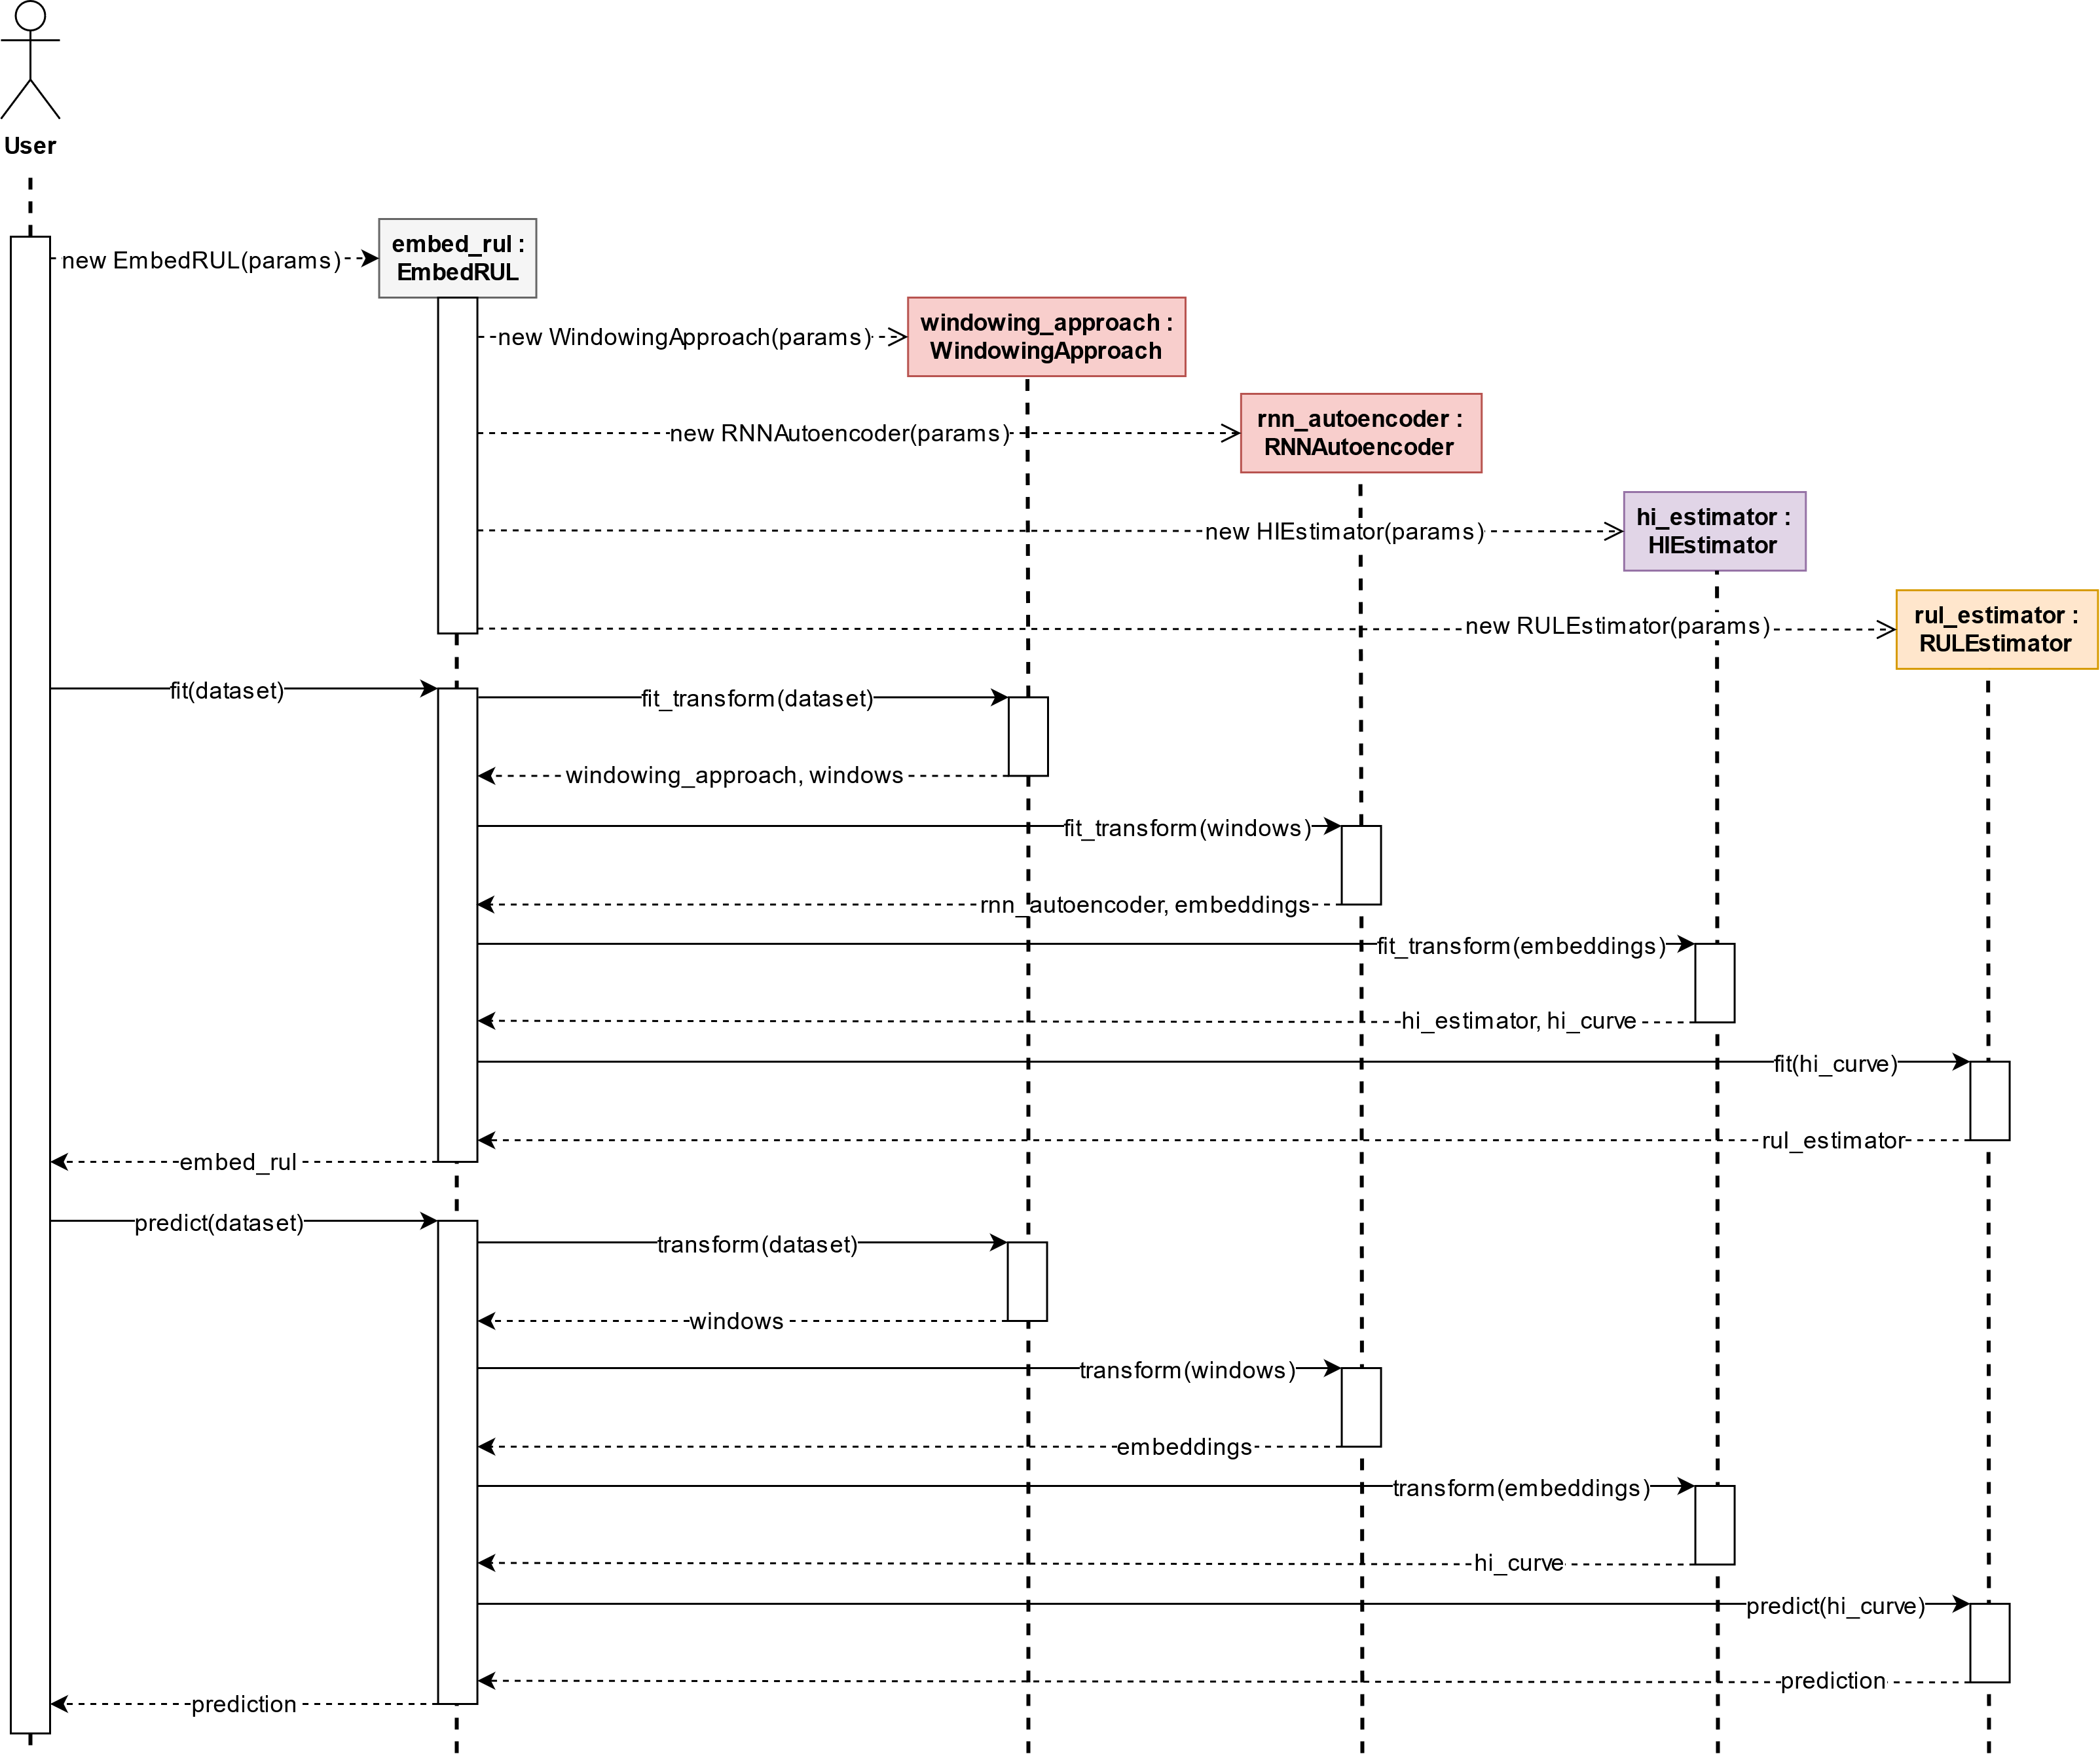
\includegraphics[width=\textwidth]{gfx/rul_seq_embed_rul}
    \caption{Sequence diagram of the Embed RUL class for fit and predict use case.}
    \label{fig:rul_seq_embed_rul}
\end{figure}

\subsubsection{Direct RUL}
\vspace*{-12.5mm}\hfill{\fontfamily{phv}\normalsize\emph{Vinay Kaundinya}}

Figure \ref{fig:rul_seq_direct_rul} shows how the \textit{DirectRUL} class first initializes \textit{WindowingApproach} and then initializes an \textit{SVR}, as a pipeline. The output of windowing approach is then passed to SVR as input. The same pipeline execution happens in both the \textit{fit} and \textit{predict} method to finally generate a RUL prediction.
\begin{figure}[H]
    \centering
    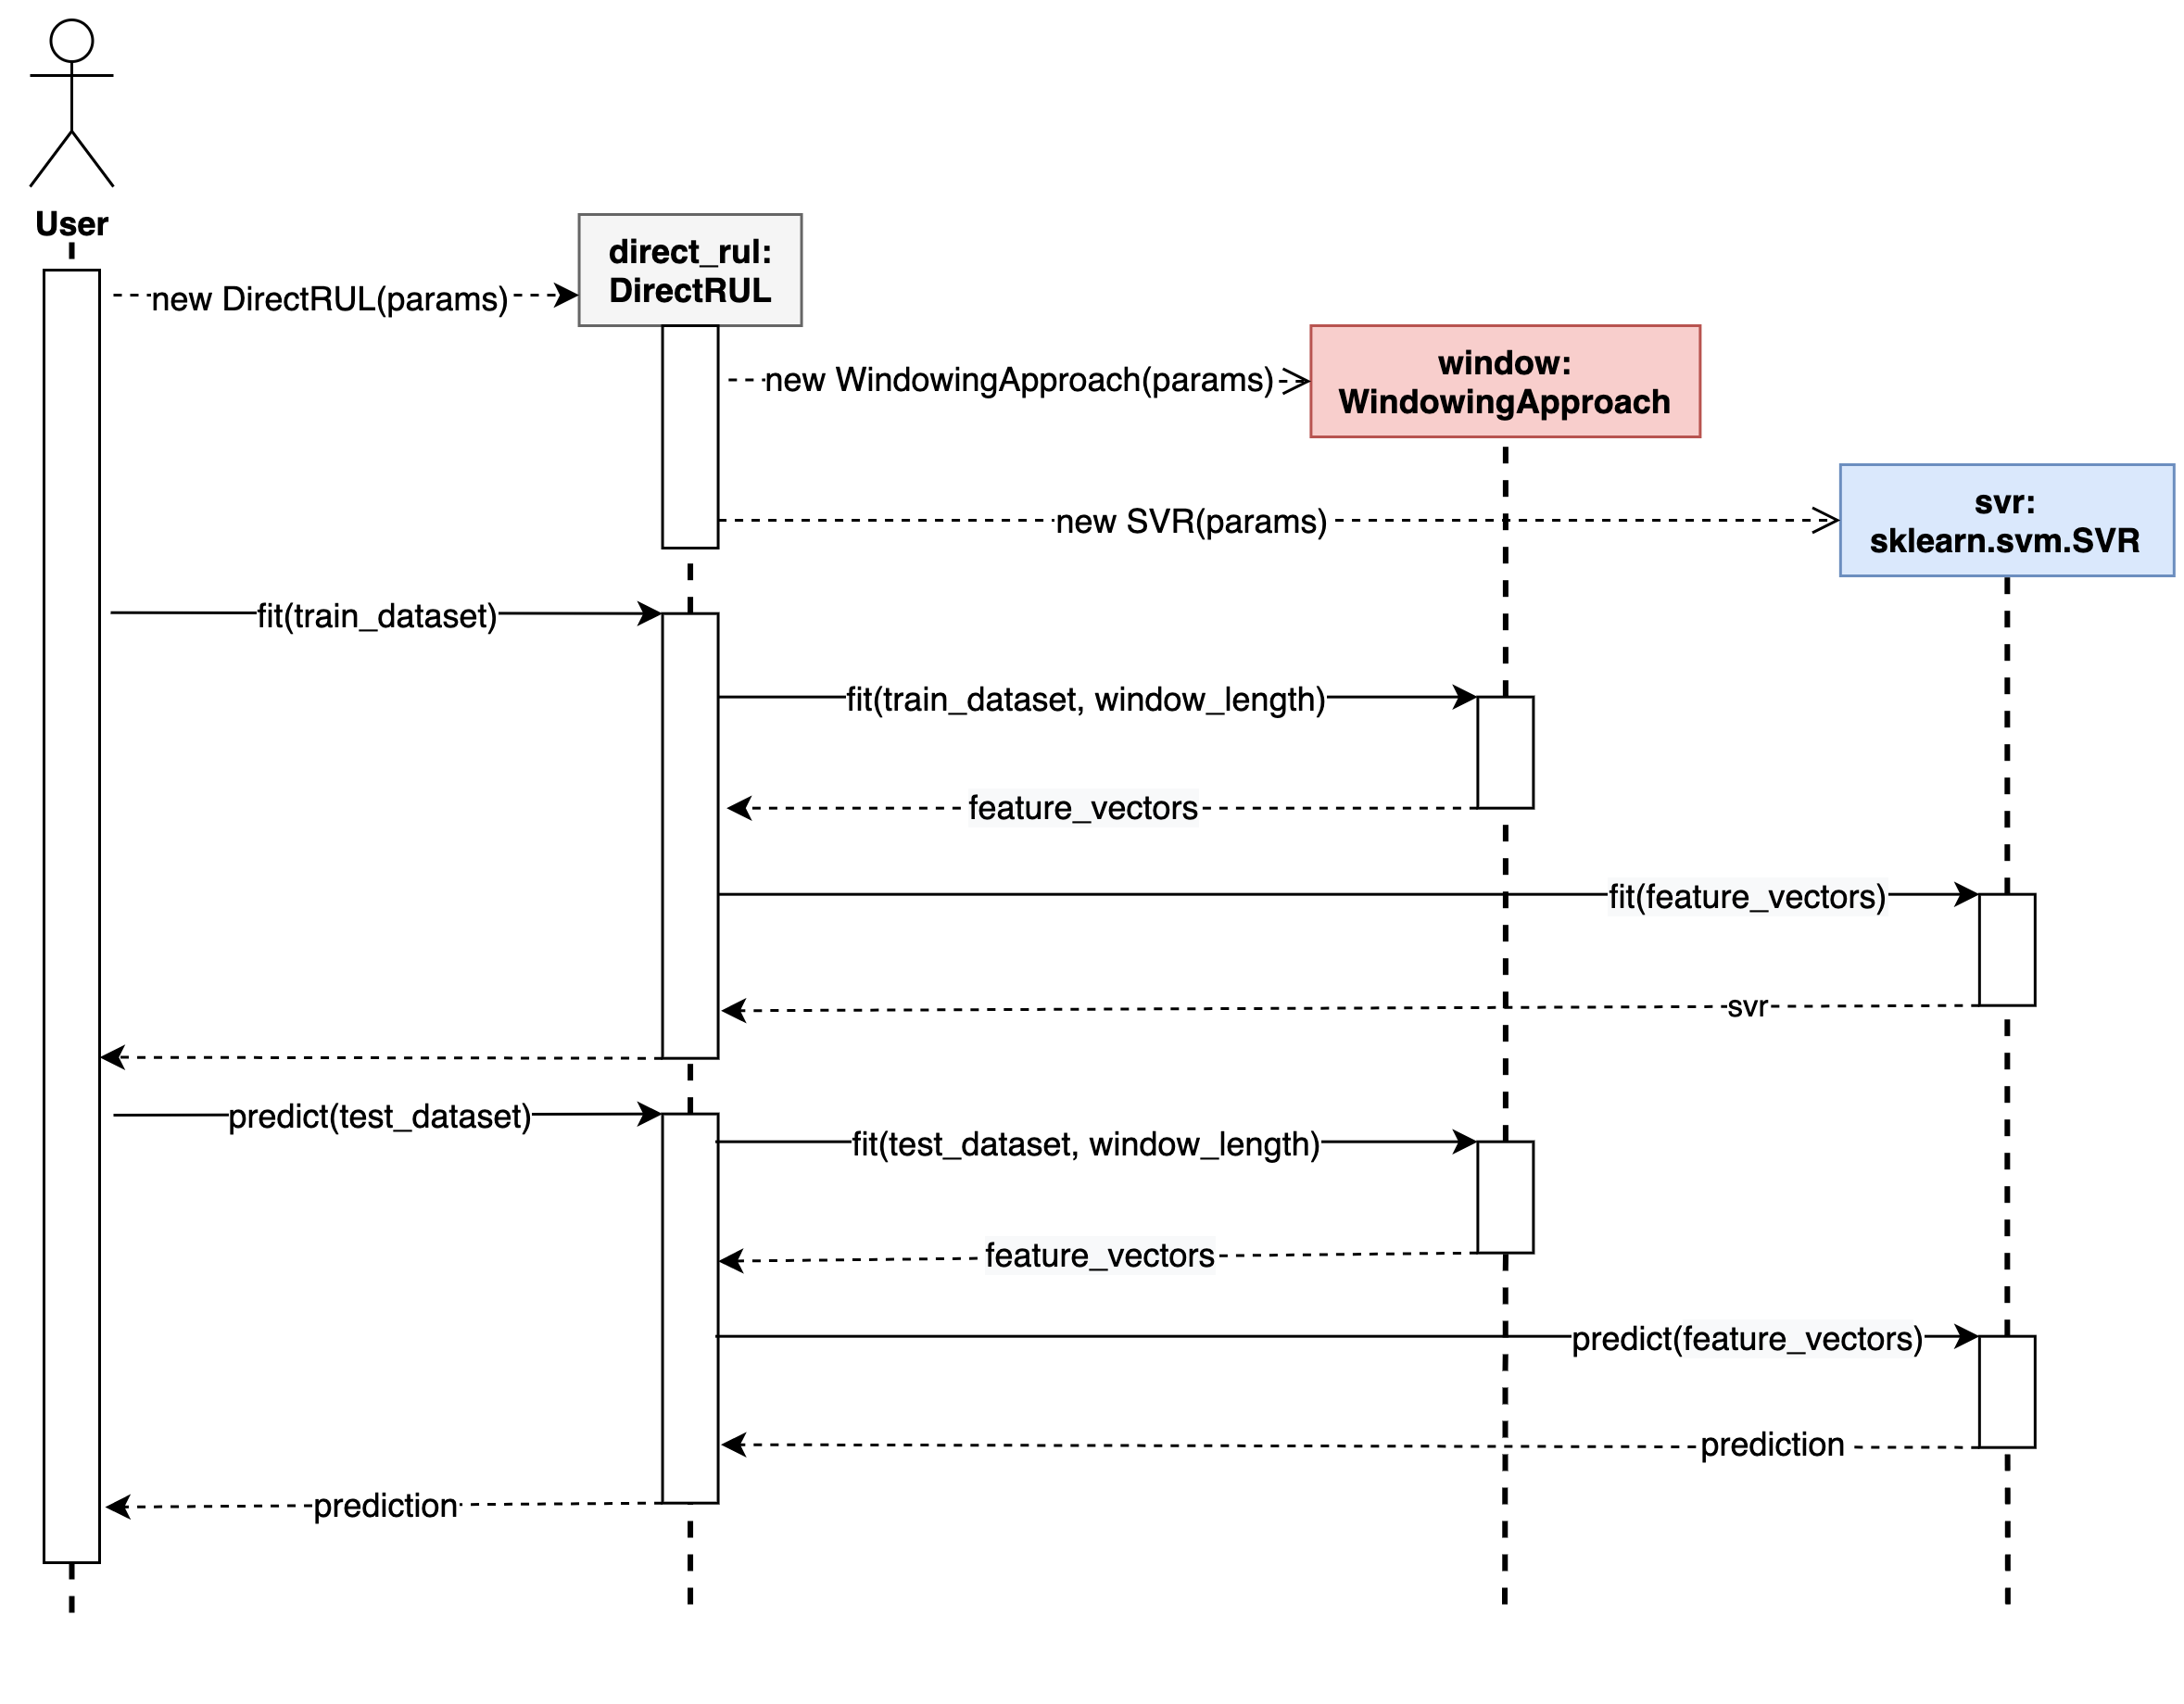
\includegraphics[width=\textwidth]{gfx/rul_seq_direct_rul}
    \caption{Sequence diagram of the direct RUL class for fit and predict use case.}
    \label{fig:rul_seq_direct_rul}
\end{figure}

\subsubsection{CNN}
\vspace*{-12.5mm}\hfill{\fontfamily{phv}\normalsize\emph{Vinay Kaundinya}}

Figure \ref{fig:rul_seq_cnn} shows how the \textit{CNN} class initializes \textit{WindowingApproach} and then initializes \textit{nn}(neural network module), as a pipeline. The output of windowing approach is then passed to neural network as input. The same pipeline execution happens in both the \textit{fit} and \textit{predict} method to finally generate a RUL prediction.
\begin{figure}[H]
    \centering
    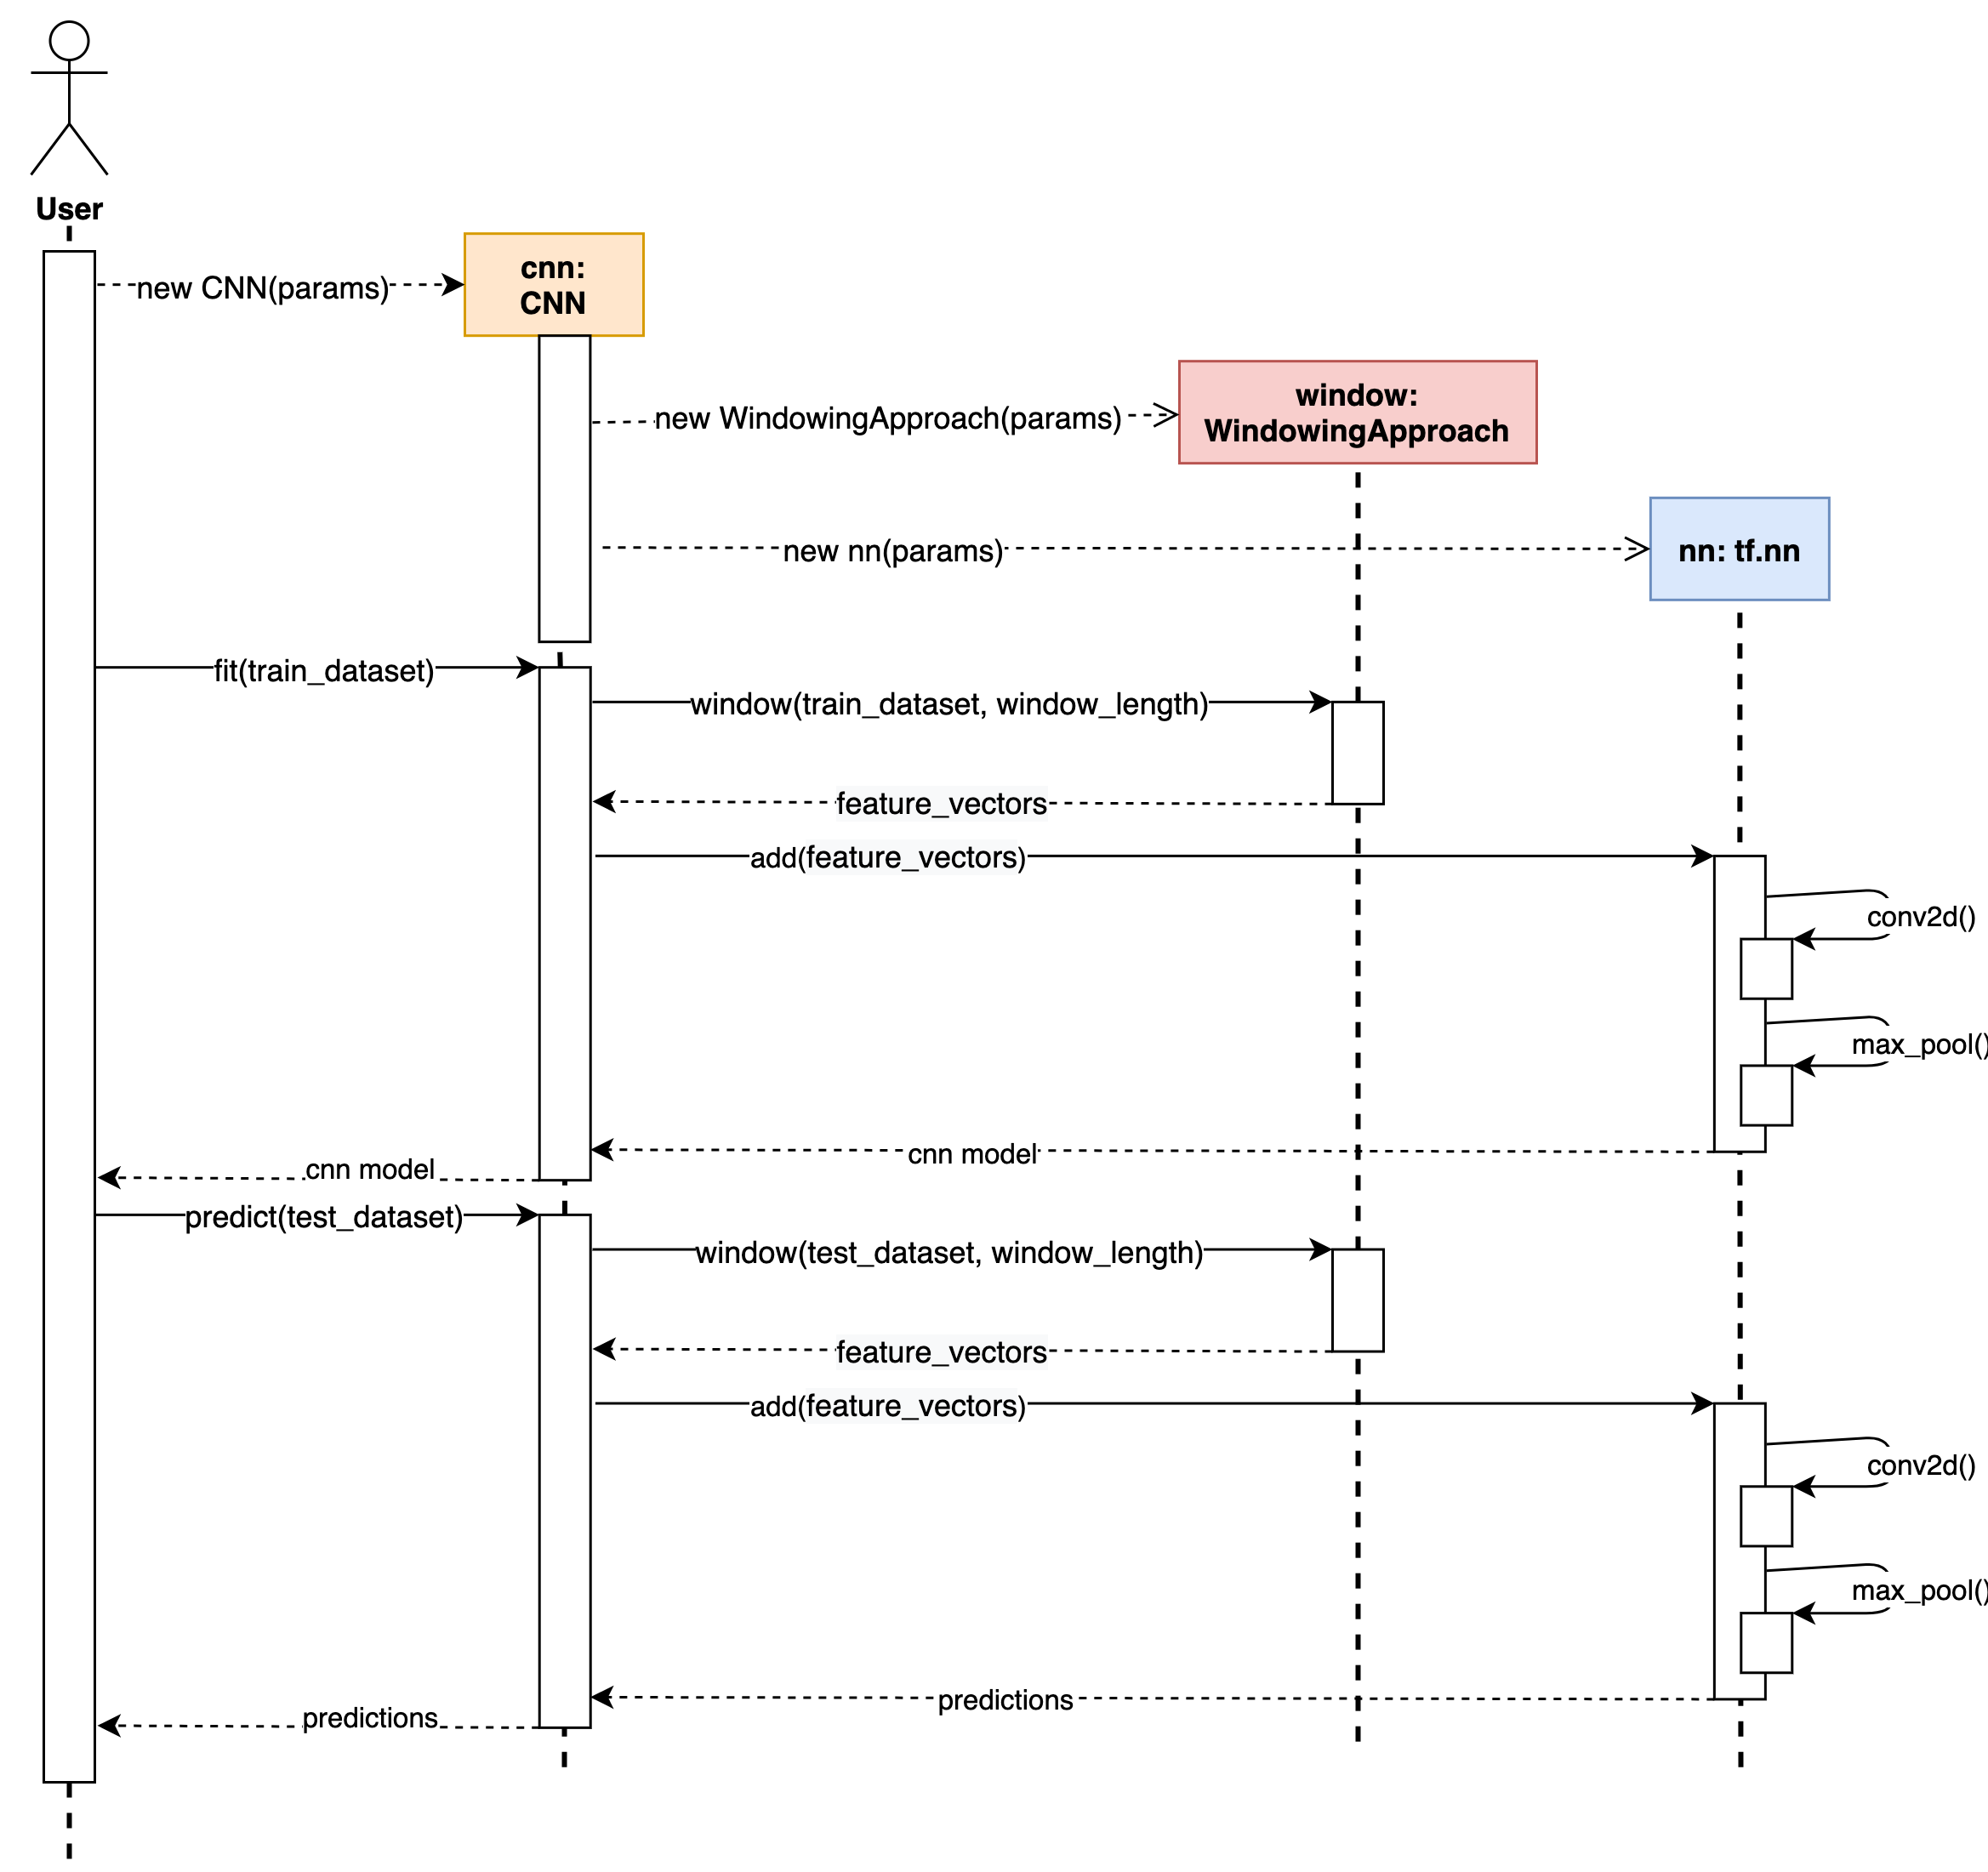
\includegraphics[width=\textwidth]{gfx/rul_seq_cnn}
    \caption{Sequence diagram of the CNN class for fit and predict use case.}
    \label{fig:rul_seq_cnn}
\end{figure}

\subsubsection{LSTM Approach}
\vspace*{-12.5mm}\hfill{\fontfamily{phv}\normalsize\emph{Vinay Kaundinya}}

In the figure \ref{fig:rul_seq_lstm}, \textit{LSTM} class initializes \textit{MinMaxScaler}, \textit{StandardScaler} and then initializes an instance of \textit{tf.keras.layers}. It shows that the dataset is passed through the two scalers before passing them into layers of LSTM.
\begin{figure}[H]
    \centering
    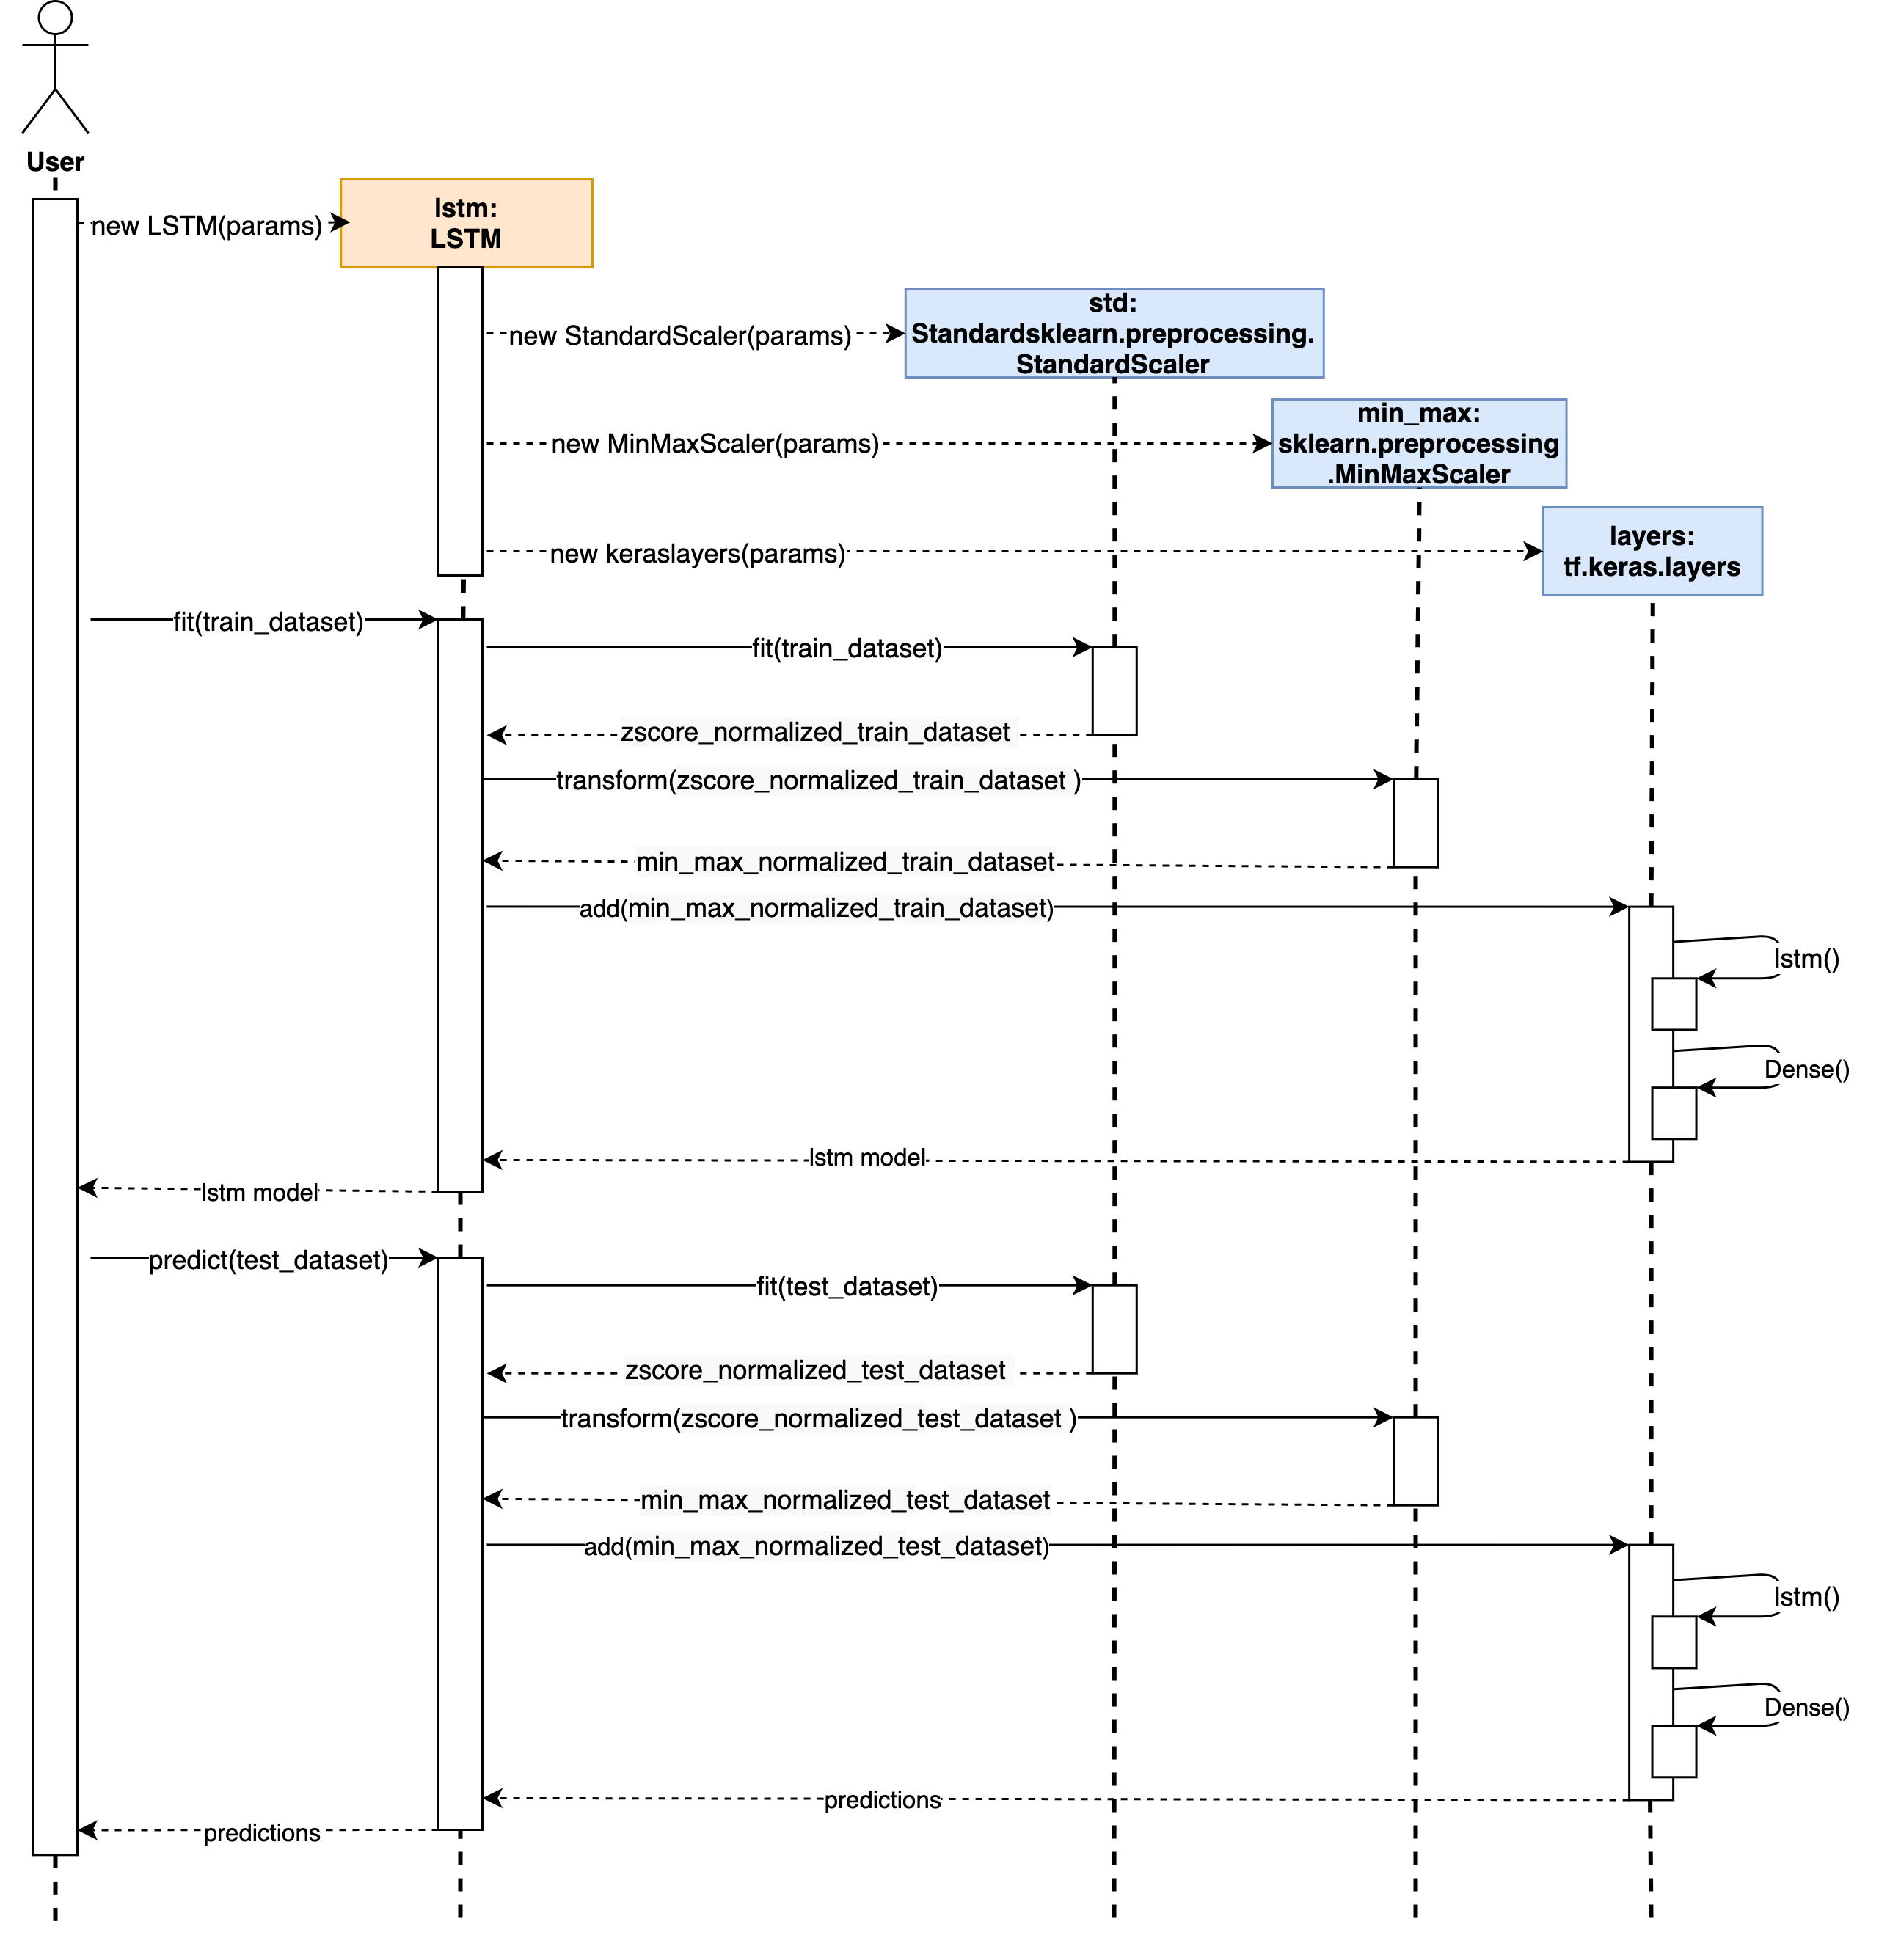
\includegraphics[width=\textwidth]{gfx/rul_seq_lstm}
    \caption{Sequence diagram of the LSTM class for fit and predict use case.}
    \label{fig:rul_seq_lstm}
\end{figure}